\documentclass[12pt,english,cucitura,oneside]{toptesi}
\usepackage[T1]{fontenc}
\usepackage[utf8]{inputenc}
\usepackage[english]{babel}
%\usepackage{hyperref}
\usepackage[colorlinks,urlcolor=Red,linktocpage,citecolor=MidnightBlue, linkcolor=MidnightBlue]{hyperref}
\usepackage{graphicx}
\usepackage{float}
\usepackage{amsmath}
\usepackage{amssymb}% http://ctan.org/pkg/amssymb
\usepackage{pifont}% http://ctan.org/pkg/pifont
\newcommand{\cmark}{\ding{51}}%

\usepackage{caption}
\captionsetup{tableposition=top,figureposition=bottom,font=small,width=.85\textwidth} %
\usepackage{amsmath}
\usepackage{subfigure} 
\usepackage{amssymb}
\usepackage{booktabs}
\usepackage{xspace}
 \usepackage[titletoc]{appendix}
\usepackage{multirow}
\usepackage{listings}
\lstloadlanguages{Python}
\usepackage{color}
\newcommand{\xmark}{\text{\ding{55}}}
\definecolor{mygreen}{rgb}{0,0.6,0}
\definecolor{mygray}{rgb}{0.5,0.5,0.5}
\definecolor{mymauve}{rgb}{0.58,0,0.82}

\lstset{ 
	backgroundcolor=\color{white},   % choose the background color; you must add \usepackage{color} or \usepackage{xcolor}; should come as last argument
	basicstyle=\footnotesize,        % the size of the fonts that are used for the code
	breakatwhitespace=false,         % sets if automatic breaks should only happen at whitespace
	breaklines=true,                 % sets automatic line breaking
	captionpos=b,                    % sets the caption-position to bottom
	commentstyle=\color{mygreen},    % comment style
	deletekeywords={...},            % if you want to delete keywords from the given language
	escapeinside={\%*}{*)},          % if you want to add LaTeX within your code
	extendedchars=true,              % lets you use non-ASCII characters; for 8-bits encodings only, does not work with UTF-8
	frame=single,	                   % adds a frame around the code
	keepspaces=true,                 % keeps spaces in text, useful for keeping indentation of code (possibly needs columns=flexible)
	keywordstyle=\color{blue},       % keyword style
	language=Octave,                 % the language of the code
	morekeywords={*,...},            % if you want to add more keywords to the set
	numbers=left,                    % where to put the line-numbers; possible values are (none, left, right)
	numbersep=5pt,                   % how far the line-numbers are from the code
	numberstyle=\tiny\color{mygray}, % the style that is used for the line-numbers
	rulecolor=\color{black},         % if not set, the frame-color may be changed on line-breaks within not-black text (e.g. comments (green here))
	showspaces=false,                % show spaces everywhere adding particular underscores; it overrides 'showstringspaces'
	showstringspaces=false,          % underline spaces within strings only
	showtabs=false,                  % show tabs within strings adding particular underscores
	stepnumber=2,                    % the step between two line-numbers. If it's 1, each line will be numbered
	stringstyle=\color{mymauve},     % string literal style
	tabsize=2,	                   % sets default tabsize to 2 spaces
	title=\lstname                   % show the filename of files included with \lstinputlisting; also try caption instead of title
}
\usepackage{afterpage}
{\setlength{\parindent}{0cm}
\usepackage[autostyle,italian=guillemets]{csquotes}
\usepackage{paracol}
\usepackage[bibstyle=numeric,citestyle=numeric,backend=biber]{biblatex}
\addbibresource{biblio.bib}
\renewcommand\arraystretch{1.25}
\linespread{1.5}
\hypersetup{%
    pdfpagemode={UseOutlines},
    bookmarksopen,
    pdfstartview={FitH},
    colorlinks,
    linkcolor={blue},
    citecolor={red},
    urlcolor={blue}
  }
% per inserire uno spazio "fantasma" nella definizione di un'abbreviazione
\usepackage{xspace}

% per inserire un DOI senza problemi coi caratteri "strani" ivi presenti
\usepackage{doi}
\renewcommand{\doitext}{DOI }% originally was "doi:"

% per inserire correttamente le unità di misura SI (incluse quelle binarie)
\usepackage[binary-units]{siunitx}
% se si desidera usare / invece che la potenza -1 per indicare "al secondo"
\sisetup{per-mode=symbol}

% per inserire codice di programmazione complesso
\usepackage{listings}% per inserire codice di programmazione complesso
\lstset{
basicstyle=\ttfamily,
columns=fullflexible,
xleftmargin=3ex,
breaklines,
breakatwhitespace,
escapechar=`
}

% modify some page parameters
\setlength{\parskip}{\medskipamount}
\advance\voffset -5mm
\advance\textheight 30mm

% riga orizzontale
\newcommand{\HRule}{\rule{\linewidth}{0.2mm}}
% esempio di creazione di semplici abbreviazioni
\newcommand{\ltx}{\LaTeX\xspace}
\newcommand{\txw}{TeXworks\xspace}
\newcommand{\mik}{MikTex\xspace}
\newcommand{\html}{HTML\xspace}

% esempio di creazione di un'abbreviazione con un parametro (il cui uso è indicato da #1)
\newcommand{\cmd}[1]{\texttt{#1}\xspace}
% per citare un RFC, es. \rfc{822}
\newcommand{\rfc}[1]{RFC-#1\xspace}
% per citare un file (es. \file{autoexec.bat}) o una URI fittizia (es. \file{http://www.lioy.it/})
% per le URI vere usare \url o \href
\newcommand{\file}[1]{\texttt{#1}\xspace}
% per inserire codice di esempio in-line
\newcommand{\code}[1]{\lstinline|#1|}
% importante per i pathname Windows perché non si può usare \ essendo un carattere riservato di Latex
\newcommand{\bs}{\textbackslash}
% definizione di un termine: formattazione ed inserimento nell'indice
\newcommand{\tdef}[1]{\textit{#1}\index{#1}}
% meta-termine, usato tipicamente nelle definizioni dei tag
\newcommand{\meta}[1]{\textit{#1}}

\begin{document}
\english
\thispagestyle{empty}
\begin{center}
\Large{\textbf{POLITECNICO DI TORINO} \\}
\vspace{0.3cm}
\large{Corso di laurea in Ingegneria Aerospaziale\\}
\vspace{0.5cm}
\Large{Tesi di Laurea Magistrale\\}
\vspace{0.3cm}
\textbf{\LARGE{Development of a Code for Aeroelastic Optimization of Wings with Stress Constraints Aggregation\\}}
\end{center}
\vspace{0.1cm}
\begin{figure}
\centering

\includegraphics[width=2in]{./Immagini/polito.png}
\end{figure}
\vspace{0.1cm}
\begin{flushleft}
\large{
\textbf{Relatori}\\
Prof. Enrico Cestino\\
Prof. Giacomo Frulla
\vspace{0.1cm}}
\end{flushleft}
\begin{flushright}
\vspace{0.1cm}
\large{\textbf{Candidato}\\
Almerico Iacono}
\end{flushright}
\vspace{0.1cm}
\begin{center}
\large{
\textbf{Supervisore esterno\\
ISAE SUPAREO}\\
Prof. Joseph Morlier\\}
\vspace{0.1cm}
\large{Ottobre 2018}
\end{center}

\newpage
\null\vspace{\stretch{1}}
\begin{flushright}
Dedica\\
\textit{A mia mamma \\
per il suo costante supporto.}
\end{flushright}
\null\vspace{\stretch{2}}
\newpage

\begin{abstract}
The development of an open-source code for the multidisciplinary design optimization related to the aero-structural optimization of wings is presented. This work is the result of a series of studies done thanks to the cooperation of ISAE and ONERA. The aim of this work is to develop an optimization process able to maximize the performance of a wing modifying its geometry out of respect of the constraints imposed, considering the aeroelastic coupling between aerodynamics loads and structural displacements. In order to manage a huge number of constraints, a constraint aggregation method is presented, based on the Kreisselmeier-Steinhauser function. It’s also presented a reduced model in relation to the aeroelastic coupling in order to reduce the computational cost. The code is entirely written in Python, while external softwares are used in order to perform aerodynamic or structural analysis.  Practical examples on common wings, like the Goland wing or NASA Common Research Wing CRM is presented.
\end{abstract}

\tableofcontents
\listoffigures

\mainmatter
\chapter*{Acknowledgements} 
\label{ring}
I would like to say thank to my supervisors Joseph Morlier and Joan Mas Colomer for the extraordinary support, technical advise and for giving me the opportunity to join their project and to join their amazing research group. They was always ready to help with clarification, allowing me to acquire knowledge. Thanks to their support I was able to grow and improve my technical knowledge. I want to say thank also to the ISAE SUPAREO, and Institut Clément Ader to guest me in this period in Toulouse.\\
My thanks also go to professor Enrico Cestino and Giacomo Frulla and Ing. Claudia Bruni, to give me the possibility to participate to this project and for the support I've had every time I've asked for it.\\
I have to say thanks also to all the extraordinary people that i meet during the university experience, for the nice time that we spent together, for the mutual assistance throughout university period and for the friendship born from this.\\
Special thanks also go to the friends I met in Toulouse, for making this experience perfect and  for the extraordinary friendship that was born and that did not stop when returned.\\
However, the biggest thanks is for my extraordinary family and for their endless support in all forms that may exist.

\chapter{Introduction to Aerostructural Optimization } 
\label{chapter1}
\section{Multidisciplinary Design Optimization MDO}
The multidisciplinary design optimization \textbf{MDO} is a field of engineering that uses optimization method in design problems incorporating an high number of disciplines. \\
Due to its multidisciplinary nature, aircraft design problems is one of the first application of the MDO.
Aerospace vehicles are extremely complex systems, and their design needs the detailed consideration of disciplines such as aerodynamics, structural mechanics, materials, control, propulsion, etc ... and the interacting between this disciplines.\\
The MDO thus makes it possible to perform a design process ( determinate the value of the design variables ) joined to an optimization process ( find the value of design variables to obtain the best value for the objective function under constraints) in view of the interaction of the different disciplines involved in the process.\\
<<The main motivation for using MDO is that the performance of a multidisciplinary system is driven not only by the performance of the individual disciplines but also by their interactions.>> \cite{mart}
\\
\begin{figure}[H]
	\centering
	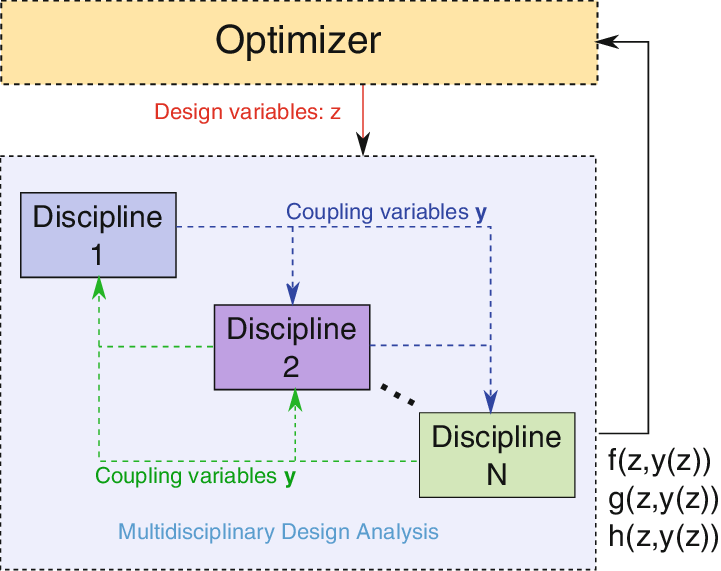
\includegraphics[width = .5\textwidth]{./Immagini/1_2.png}
	\caption{MDO scheme}
	\label{fig:1_1}
\end{figure}
Solving MDO problem in the early phase of the design process, by the support of advanced computational analysis tools, can improve the design and provide reduction of time and cost of the design cycle.\\
One of the first applications of the MDO was aircraft wing design, where there is a strong coupling between aerodynamics and structures, the aeroelastic coupling. After the application of MDO have been extended to the complete aircraft and to other field.\\
In MDO is important to define the architecture of the process,how organize the optimization software, the disciplines and the analysis of the model and the approximation model. So can be distinct two different architecture, the monolithic and the distributed. In the monolithic approach just one optimization problem will be solved, instead in the distributed approach there re multiple subproblem, which contain less variables and constraint, so the reaserch of the optimum of the main problem is split in the solving of little problems. So to solve the same optimal design problem there are many ways, and the choise of the architecture entails the computational cost and the final optimum design.

\subsection{Optimization Methods}

Computational design procedures are based on numerical analysis methods that evaluate the relative merit of a set of feasible designs. The merit of a design is based on the value of an objective function that is computed using numerical simulations such as CFD and CSM programs. The choice of objective function is extremely important and requires a deep knowledge of the multidisciplinary design problem at hand. \cite{mart2}
\\
A typical example of a constrained optimization problem can be represent as:

\begin{align*}
	&minimize \ \ F(x_i)\\
	&w.r.t. \ \ \ \ \ \ \ \ \ \ x_i  \ \ \ \ \ \ \  i=1,2,..,N\\
	&subject\   to\ \  G_m(x_i) \ \ m=1,2,...,M
\end{align*}

where $F$ is a non linear function of the $N$ design variables $ x_i $, and $ G_m $ are the $ M $ nonlinear inequality constraints to be respected. For a given design problem , a number of parameters $ x_i $ are allowed to change. Optimization algorithms is based to finding the design variables that yield the optimum.
In our project we use the MDO to find the best configuration for a given wing taking account of the aeroelastic coupling, respecting a set of constraint.\\

There are a lot of optimization algorithms, but they can be classified in two categories:
\begin{itemize}
	\item \textbf{gradient free}: the research of the optimum value is based just on the value of the objective function
	\item \textbf{gradient based}: the algorithm use over the value of the objective function also its gradient with respect to the design parameters
\end{itemize}
\subsubsection{Gradient Free Methods}
Between the gradient free methods there is the grid searching, where the design space is surveyed by evaluating each point in a multidimensional grid;the problem of this method is that the required number of evaluation of the objective function grow exponential with the number of design variables, so it's not worth to use this method when the design variables is more than a few. An alternative is the random search, where is not needed an high number of evaluation, but is not guarantee that the optimum value will be found, also for an high number of evaluation. The most used methods is the non linear simplex; to create a simplex is necessary to evaluate $N+1$ points in a $N-$dimensional space; the simplex evolves exploring the design space searching a better point, but also this method became useless if the design parameters is more than half dozen.\\
Ultimately the gradient free method is a powerful instruments to set an fast optimization but they became inefficient when the number of the design parameters is high.\\
\subsubsection{Gradient Based Methods}
In the second category we have the gradient based methods; this methods is characterized by the knowledge of the gradient of the objective function respect the design variables. That methods need a first and sometimes second order sensitivity analysis, with that information it can move into the design space with criteria, that will lead to the optimum. The great advantage of these methods is that they converge to the optimum with a significantly smaller number of objective function evaluation. On the other hand these methods work well only when the objective function changes smoothly with the design variables, and the convergence is guarantee just for a local minimum. The simple example of a gradient based method is the steepest descend, where the optimization step are choose in the direction of the gradient vector. Instead the Newton method require the Hessian Matrix, so a second order sensitivity information, in addition to the first derivatives, but it show an higher rate of convergence. A middle step is the Quasi-Newton, where the Hessian Matrix is approximated using conjugate gradient. Overall all of these method use the sensitivity analysis to identify the right direction in the design space and than perform a one-dimensional optimization in that direction before search a new direction.\\
\\
Both of these methods are used currently, and the choice depends on the problem, for problems with small set of variables but with multiple local minima or discontinues the gradient free methods are more suitable, instead for problem where the number of variables is pretty high, like high fidelity aerodynamics shape optimization a gradient based method is the best option.
\subsection{Sensitivity Analysis}
A possible definition of sensitivity analysis is the following: "The study of how the uncertainty in the output of a model (numerical or otherwise) can be apportioned to different sources of uncertainty in the model input."\cite{salt}\\\
In our case sensitivity analysis consist in determining derivatives of one or more quantities, the objective functions, compared to the independent variables, the design parameters. Know these derivatives it's necessary for the gradient based algorithm. The determination of the gradient it's the most expansive operation in the optimization process, so it's important to use efficient methods to do the sensitivity analysis, to obtain high accurate gradients with the minimum computational cost.\\
There are different sensitivity analysis methods, with pros and cons, and the correct choice depends on the problem (number of independent variables and output, and how it affects the computational expense and scalability of the method ), th importance of the computational efficiency and the amount of the human support.
Let's see the most common method used for the sensitivity analysis:
\subsubsection{Finite Differences}
One of the common method to estimate the gradient is the finite differences method. This method is not particularly accurate and computationally efficient, but his implementation is  really easy, that's why it found a large use in the design process with a huge number of variables.\\
All the finite differences formulas derive from the Taylor series expansion, by truncating it at the order of interest. The first order approximation, usinf the \textit{foward difference} is given by:
\begin{equation*}
\frac{df(x_i)}{dx_i}= \frac{f(x_i + h ) - f(x_i	)}{h}+\mathcal{O}(h)
\end{equation*}
where $h$ is the finite difference step, $x_i$ is the point where the derivate is evaluate and $f$ is the function which we want to compute the gradient.
\subsubsection{Complex-Step Derivate Approximation}
The complex-step derivative approximation is a relatively new method that unlike finite differences is extremely robust to changes in the step size \cite{mart2}. The approximation of the first derivative can be obtained from complex calculus and represented by the formula :
\begin{equation*}
\frac{df(x_i)}{dx_i}=\frac{Im[f(x_i+jh)]}{h}+\mathcal{O}(h^2)
\end{equation*}
where the imaginary part of the function evaluation is obtained by a perturbation with a pure imaginary step, and dividing by h a second order approximation is reached.\\
The computational cost, as the finite difference method, is proportional to the number of variables $N$, but a complex arithmetic is required, so generally the cost is twice than the cost for finite differences.
\subsubsection{Analytic Methods}
The analytics methods are the most accurate and efficient methods for sensitivity analysis. But they are also the most expansive methods, because to determinate the gradients of a model by analytic approach it's required to know the governing equations of the model and how to resolve it. Usually it's hard to implement an algorithm capable to calculate the gradient, so it's required the human support to determinate it, alternatively is possible to use algorithms that solves the corresponding sensitivity equation, like the adjoint methods. That kind of method is appreciated because the cost to computing gradient is independent of the number of design variables, so it's a right chose for problem where a large number of design variables is engaged.
\section{Aeroelasticity}

Aeroelasticity is the science which studies the interaction among inertial, elastic and aerodynamic forces acting upon a flexible structure exposed to a fluid flow. It was defined by Arthur Roderick Collar in 1947 as "the study of the mutual interaction that takes place within the triangle of the inertial, elastic, and aerodynamic forces acting on structural members exposed to an airstream, and the influence of this study on design.".\\
This interaction is described by the Collar aeroelastic triangle Fig.\ref{fig:1_2}

\begin{figure}[H]
\centering
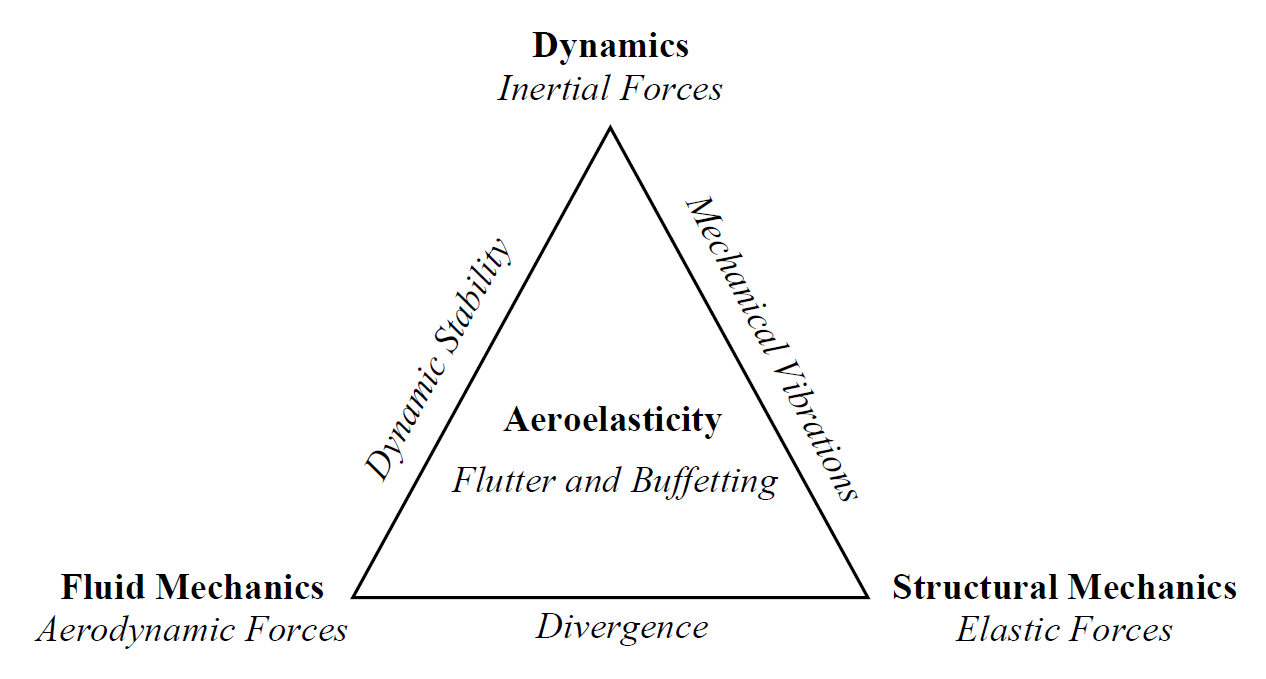
\includegraphics[width = .43\textwidth]{./Immagini/1_1.png}
\caption{Collar Triangle}
\label{fig:1_2}
\end{figure}
The interaction between these three forces can cause several undesirable phenomena like
divergence (static aeroelastic phenomenon), 
flutter (dynamic aeroelastic phenomenon), 
limit cycle oscillations (nonlinear
aeroelastic phenomenon), 
vortex shedding, buffeting, galloping
(unsteady aerodynamic phenomena) .
\subsection{Static aeroelasticity}
The interaction between the aerodynamic forces ans the elastic forces determine the static aeroelasticity phenomena. In this work we are principally interested to the aeroelastic coupling, the aerodynamic force induce on the wing a structural deformation, which modify the geometry of the wing, and then the aerodynamic forces. So to determinate correctly the aerodynamic forces it's necessary to determinate it whit an iterative process, where step by step the forces and the deformation are updated, until the convergence is reached.\\
A typical aeroelastic problem can be described by the following matrix equation:
\begin{equation*}
[M]\mathbf{\ddot{q}}+[C]\mathbf{\dot{q}}+[K]\mathbf{q}=\mathbf{F}(bs,\mathbf{q},\mathbf{\dot{q}},\mathbf{\ddot{q}},\mathbf{V},t,\omega)
\end{equation*}
where $[M]$ is the mass matrix, $[C]$ is the damping matrix, $[K]$ is the stiffness matrix, $\mathbf{\ddot{q}},\ \mathbf{\dot{q}},\ \mathbf{q}$ are the degree of freedom( and the first and second time derivatives), $\mathbf{\textbf{F}} $ is the aerodynamic force, $\mathbf{V}$ is the air speed, $t$ is the time, $\omega$ is the oscillation frequency and $bs$ indicate bodyshape, and define the join between the aerodynamic forces and the shape of the structure.\\
In a static model the equation became:
\begin{equation*}
[K]\mathbf{q}=\mathbf{F}(bs,\mathbf{q},\mathbf{V})
\end{equation*}
To understand how the problem involve the study of the typical aeroelastic section can be approached.
\subsubsection{Typical Aeroelastic Section}
The typical aeroelastic section consist in a model where the wing is assumed as a 2DoF system:
\begin{figure}[H]
	\centering
	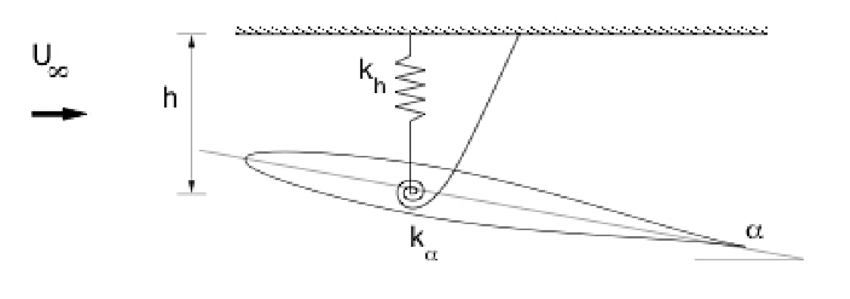
\includegraphics[width = 1\textwidth]{./Immagini/2_ala.png}
	\caption{Typical aeroelastic section}
	\label{fig:2_ala}
\end{figure}
The two DoF are the vertical translation $h$ and the rotation $\alpha$.
The stiffness is concentrated in the elastic axes, and is represented by two spring, one linear and one torsional, with respectively $K_h$ and $K{\alpha}$. Writing the equation of the rotation at the shear center we obtain:
\begin{equation*}
Wd+M{c.a.}+Le-K_{\alpha}\alpha=0
\end{equation*}
where $W$ is the weight, $d4$ the distance of the center of gravity and shear center, $e$ the distance of the aerodynamic center and shear center. Collecting the terms that depends of the rotation $\alpha$, we obtain:
\begin{equation*}
(K_{\theta}-qSC_{p,\alpha}e)\theta=M_0
\end{equation*}
where
\begin{equation*}
M_0=Wd+M{c.a.}+qSC_{p,{\alpha_0}}e
\end{equation*}
The term $K_{ae}=K_{\theta}-qSC_{p,\alpha}e$ is the aerodynamic stiffness. So in the moment when we consider the deformation of the wing the stiffness of the structure change, while the aerodynamic stiffness is coupled with the aerodynamic forces and structural displacement, so it's not possible to compute its value at the start of the process, from this an iterative method is used.\\
The divergence problem is caused from this pattern, in fact the aerodynamic stiffness reduce the stiffness of the structure, when the total stiffness reach the value of 0 the structure became instable.\\
In our work we don't consider the divergence problem, but just the aerodynamic coupling, solved by the MDA loop.

\chapter{Source Code Description} 
\label{chapter2}
The main goal of this project is to develop an open-source software to perform an aeroelastic optimization on an established wing model.\\
%Per effettuare un' ottimizzazione aeroelastica è necesserio disporre di uno strumento in grado di effettuare un' analisi strutturale, in modo da determinare l' entità delle deformazioni strutturali nonchè le tensioni generate nella struttura sotto l' azione dei carichi aerodinamici, di uno strumento in grado di effettuare un' analisi aerodinamica, che permetta di determinare l' entità delle forze aerodinamiche in funzione delle variabili di volo, di uno strumento in grado di effettuare un analisi dinamica e quindi di determinare fattori come la velocità di flutter, e gli andamenti delle frequenze proprie e dello smorzamento in funzione della velocità di volo e infine di uno strumento in grado di ottimizzare il problema, andando a modificare con criterio le variabili di design in funzione dell' effetto che queste ultime inducono nel processo e determinare quindi il valore di ottimo per tali variabili per cui si ottengano le migliori prestazioni, rispettando però i limiti imposti.\\
%Per effettuare un analisi multidisciplinare come questa sono richiesti perciò diversi software, che dovranno essere lanciati in successione più e più volte. Per tale motivo si è scelto come linguaggio di programmazione il linguaggio python, tramite il quale è possibile automatizzare al massimo tale processo, è possibile infatti configurare il programma in modo tale da compilare i file di input necessari ai diversi programmi per funzionare, lanciare tali programmi, e ottenere dai file di output i valori delle variabili desiderate.\\
%Andiamo a vedere quindi gli strumenti di cui si compone il nostro codice:
To perform aeroelastic optimization it is necessary to have an instrument capable of carrying out a structural analysis, in order to determine the extent of the structural deformations as well as the tensions generated in the structure under the action of the aerodynamic loads, of an instrument capable of to carry out an aerodynamic analysis, which allows to determine the entity of the aerodynamic forces as a function of the flight variables, of an instrument able to perform a dynamic analysis and therefore to determine factors such as flutter velocity, and frequency trends and of the damping according to the flight speed and finally of an instrument able to optimize the problem, going to modify the design variables according to the effect that the latter induce in the process and therefore determine the optimal value for these variables for which the best performances are obtained, but respecting the limits imposed. \\
To perform a multidisciplinary analysis like this, various software are required, which must be launched successively over and over again. For this reason we have chosen as the programming language the python language, through which it is possible to automate this process as much as possible, it is possible to configure the program in such a way as to compile the input files necessary for the different programs to run, launch these programs, and obtain the values of the desired variables from the output files.\\
So let's see the tools that make up our code:
\begin{itemize}
	\item \textbf{Python}: open source coding language based on class and methods
		\item \textbf{OpenMDAO}: open source library for python containing method specialised for the multidisciplinary design optimization
			\item \textbf{Panair}: open source software developed by NASA for aerodynamic analysis
				\item \textbf{Panin}: precompiler for Panair
					\item \textbf{Nastran95}: open source software developed by NASA for static and dynamic structural analysis
						\item \textbf{Gmsh}: open source software for generation of meshes
\end{itemize}


\section{Structure of the Code}
%Il modo migliore per vedere come è strutturato il codice è tramite il diagramma XDSM ( eXtended Design Structure Matrix), tool sviluppato da Lambe and Martins (citazione) che aims to represent MDO process. \\In Fig.\ref{fig:2_1} è rappresentato il diagramma XDSM relativo al nostro progetto. Nel diagramma ogni box rettangolare rappresenta un analisi (che può essere una funzione o un computational code), le cui variabili di input sono rappresentate dai box bianchi sulla sinistra, mentre le variabili di output dai box bianchi in alto, le linee grige rappresentano le data dependencies, al contrario le linee nere rappresentano process connections. Tutti i componenti sono numerati in relazione all' ordine in cui vengono eseguiti.
The best way to see how the code is structured is via the XDSM diagram (eXtended Design Structure Matrix), a tool developed by Lambe and Martins (citation) that aims to represent MDO process. \\
 In  Fig.\ref{fig:2_1} the XDSM diagram related to our project is shown. In the diagram each rectangular box represents an analysis (which can be a function or a computational code), whose input variables are represented by the white boxes on the left, while the output variables from the white boxes on the top, the gray lines represent the date dependencies, on the contrary the black lines represent process connections. All components are numbered in relation to the order in which they are executed.
%scrivere meglio guardano jose e citazione
\begin{figure}[H]
	\centering
	\includegraphics[width = 1\textwidth]{./Immagini/2_1.png}
	\caption{\textit{XDSM} Diagram of the multidisciplinary analysis and optimization process}
	\label{fig:2_1}
\end{figure}
The steps that define the optimization process are the following:
\begin{enumerate}
	\setcounter{enumi}{-1}
	\item Initiate the optimization process.
	\item  The initial geometry is created.
	\item  The interpolation matrix to couple aerodynamic and structure is created.
	\item  Initiate the coupling process between aerodynamic forces and structural displacements.
	\item Determination of the aerodynamic loads by aerodynamic analysis.
	\item  Transfer the aerodynamic forces from aerodynamic mesh to structural mesh.
	\item Determination of the structural displacements and stresses.
	\item Transfer the structural displacements from structural mesh to aerodynamic mesh.
	\item Determination of the characteristics of the wing for this configuration.
	\item  Computation of the constraints.
	\item Based on the objective and constraints value, decide the design variables value for the next optimization iteration.
\end{enumerate}
Steps 1 to 10 are repeated until the convergence of the optimization is achieved.\\

\section{Component}
In this section is explained how each component is structured. Each component is written on a different \textit{.py} file, and it will be called in the main script. Using the openMDAO structure all the variables are connected between the components by the command \textit{promotes = [*]}, so each time a component changes the value of a variable, its value will be updated for all the component.
\subsection{Geometry  }
The first component it's the geometry component, this component will create the initial geometry from a bounch of parameters specified in the main code, or in an appropriate \textit{.py} file. The user can specify the chord factor, the scale factor, the twist angle, the mid spar position and the sweep angle. From this parameters the component create and \textit{.igs} file with the parametric geometry. After it will run the program \textit{gmsh} to mesh this geometry and that meshed geometry will stored in an \textit{.bdf} file. \\
At the end of the process the component stores in a dedicated python dictionary the coordinates of the aerodynamic points, the nodes of the outer surface and the nodes and them coordinates of the finite element model, in order to be used later by other components.
\begin{figure}[H]
	\centering
	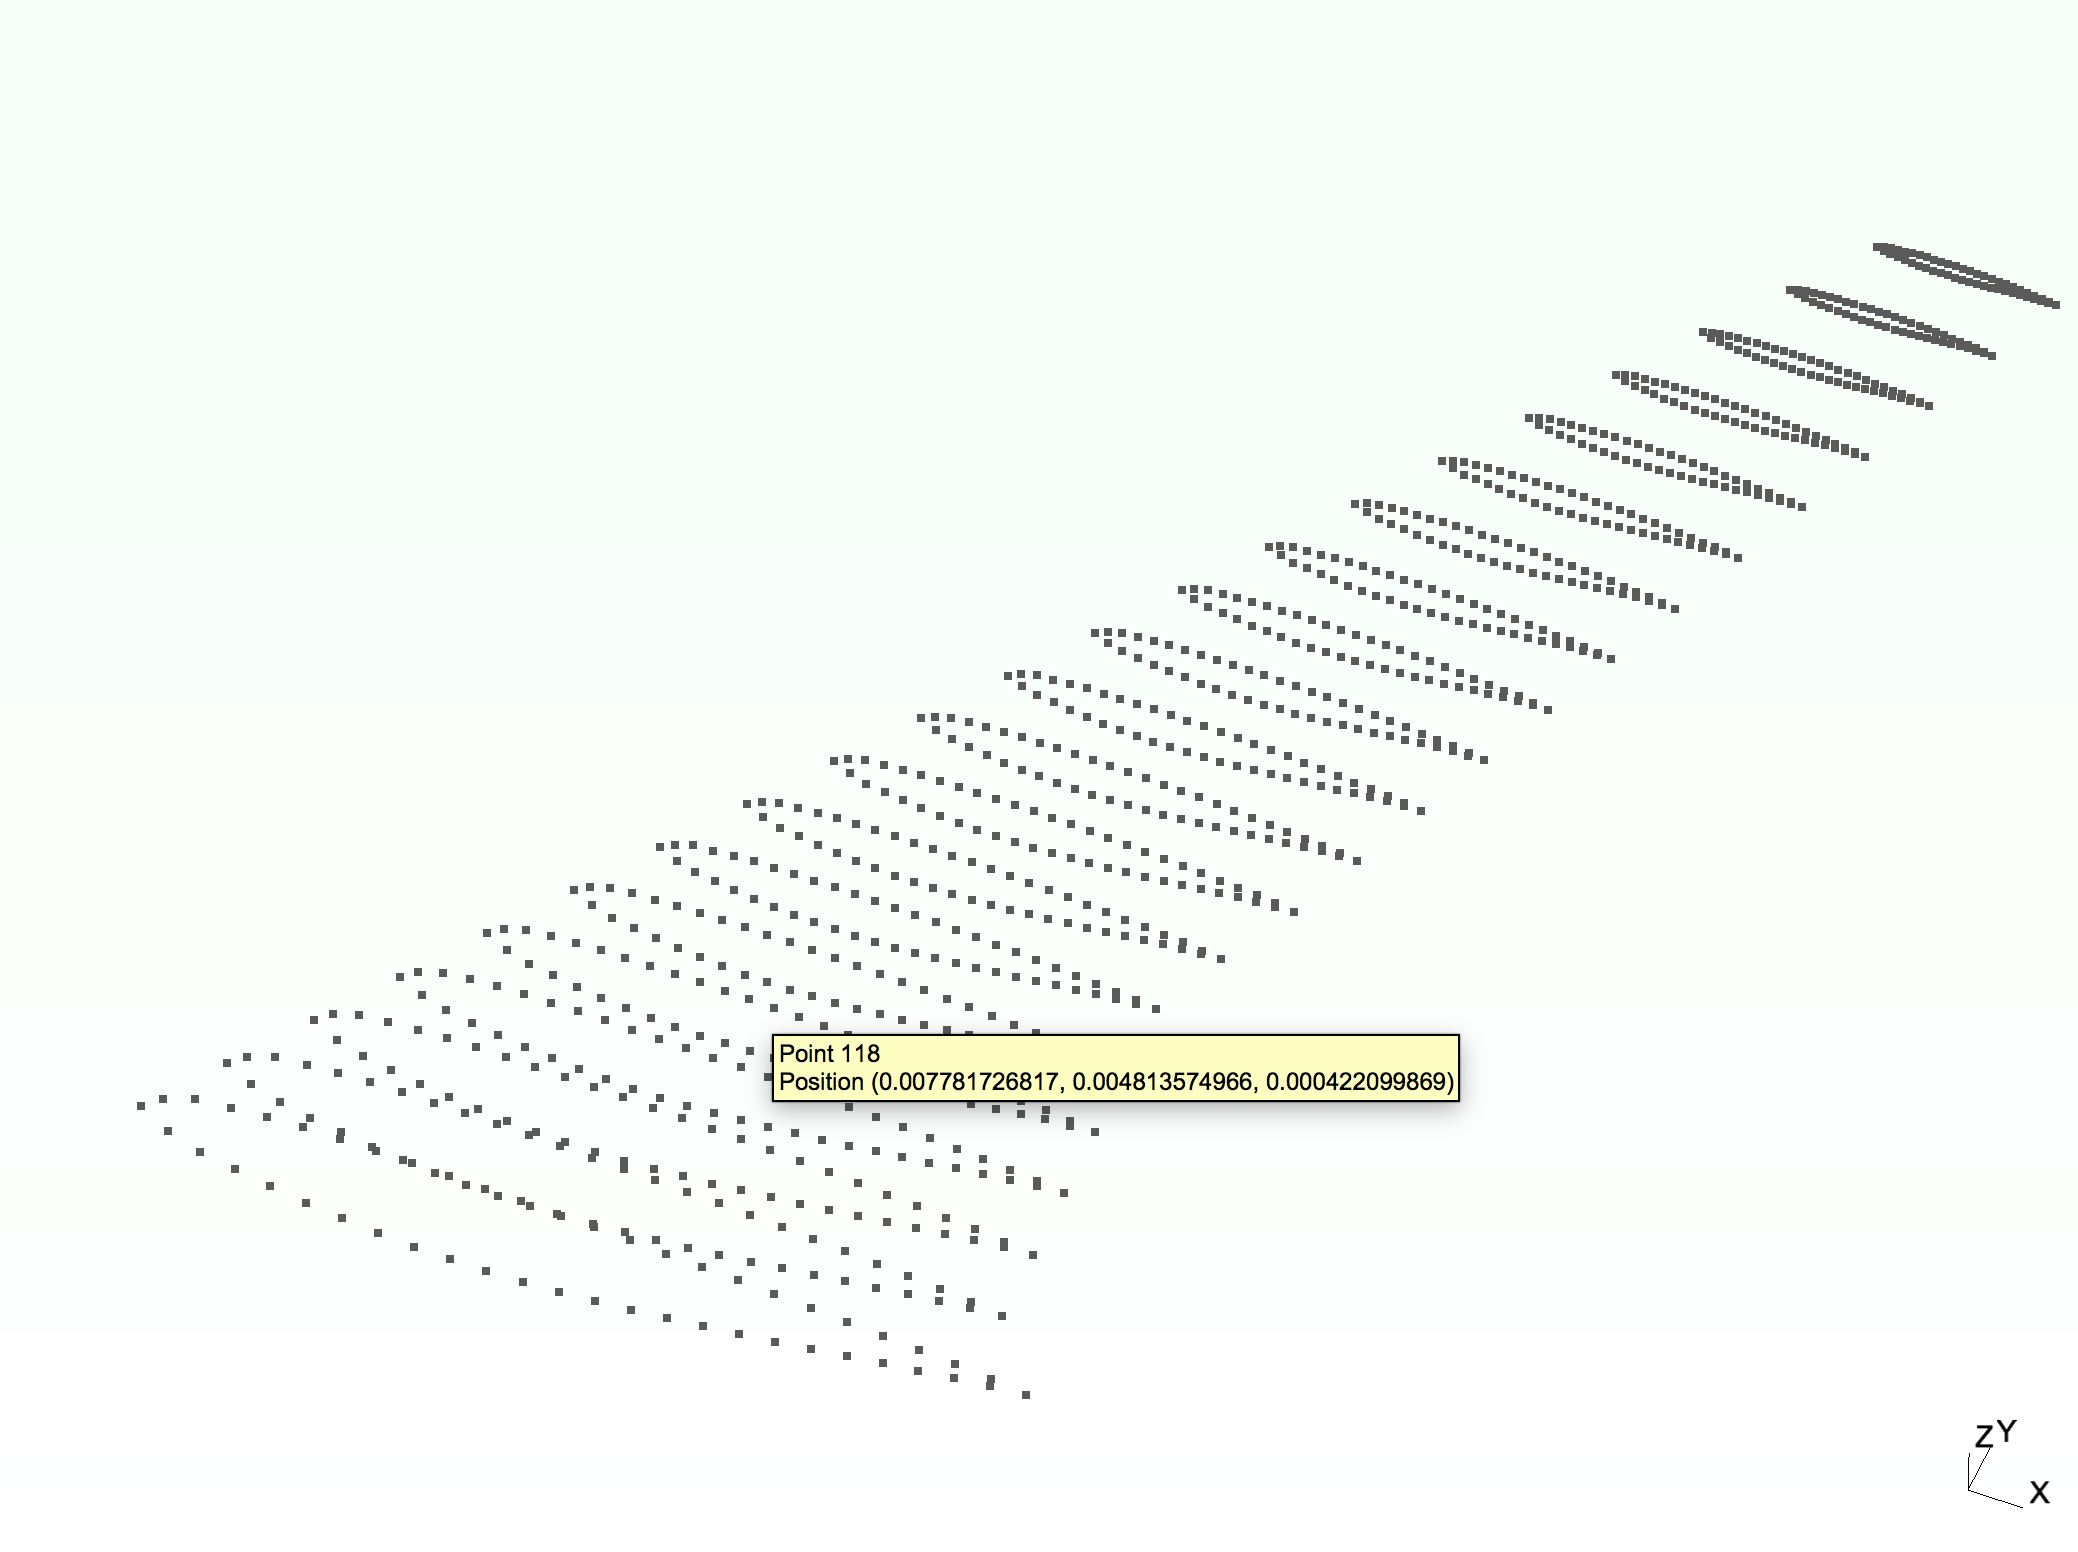
\includegraphics[width = 1\textwidth]{./Immagini/2_2.png}
	\caption{Example of .igs file created from the geometry component}
	\label{fig:2_2}
\end{figure}
\subsection{Raidial Basis Functions}
The second component is the radial basis functions, this component creates the interpolation matrix to couple the aerodynamic and structure component, in fact in the general case these grids are not coincident.The interpolation matrix is created using a fluide-structure interpolation and mesh motion scheme based on the use of radial basis functions (RBF), as the method presented in the work of Rendall and Allen \cite{all}. This displacement and load transfer techniqueis conservative in terms of total load and moment, as shown by Jakobsson and Amoignon. \cite{jac} One of the advantages of this type of interpolations is that no mesh connectivity is required between the two disciplines. This is particularly suitable for the cases where the aerodynamic and structural models do not represent the same geometries. Usually, the aerodynamic grid is based on the outer mold line, even though there may be cases where it is based on the mean camber surface only (e.g., the vortex lattice methods).\cite{joan}\\Once the interpolation matrix \textbf{H} have been created, since the dimensions of the problem will not change until the process, it will hold and it will be used each time the aerodynamic component and the structure component run in order to transfer respectively the aerodynamic forces from the CFD mesh to the FEM mesh and the nodal displacement from the FEM mesh to the CFD mesh.\\
\begin{figure}[H]
	\centering
	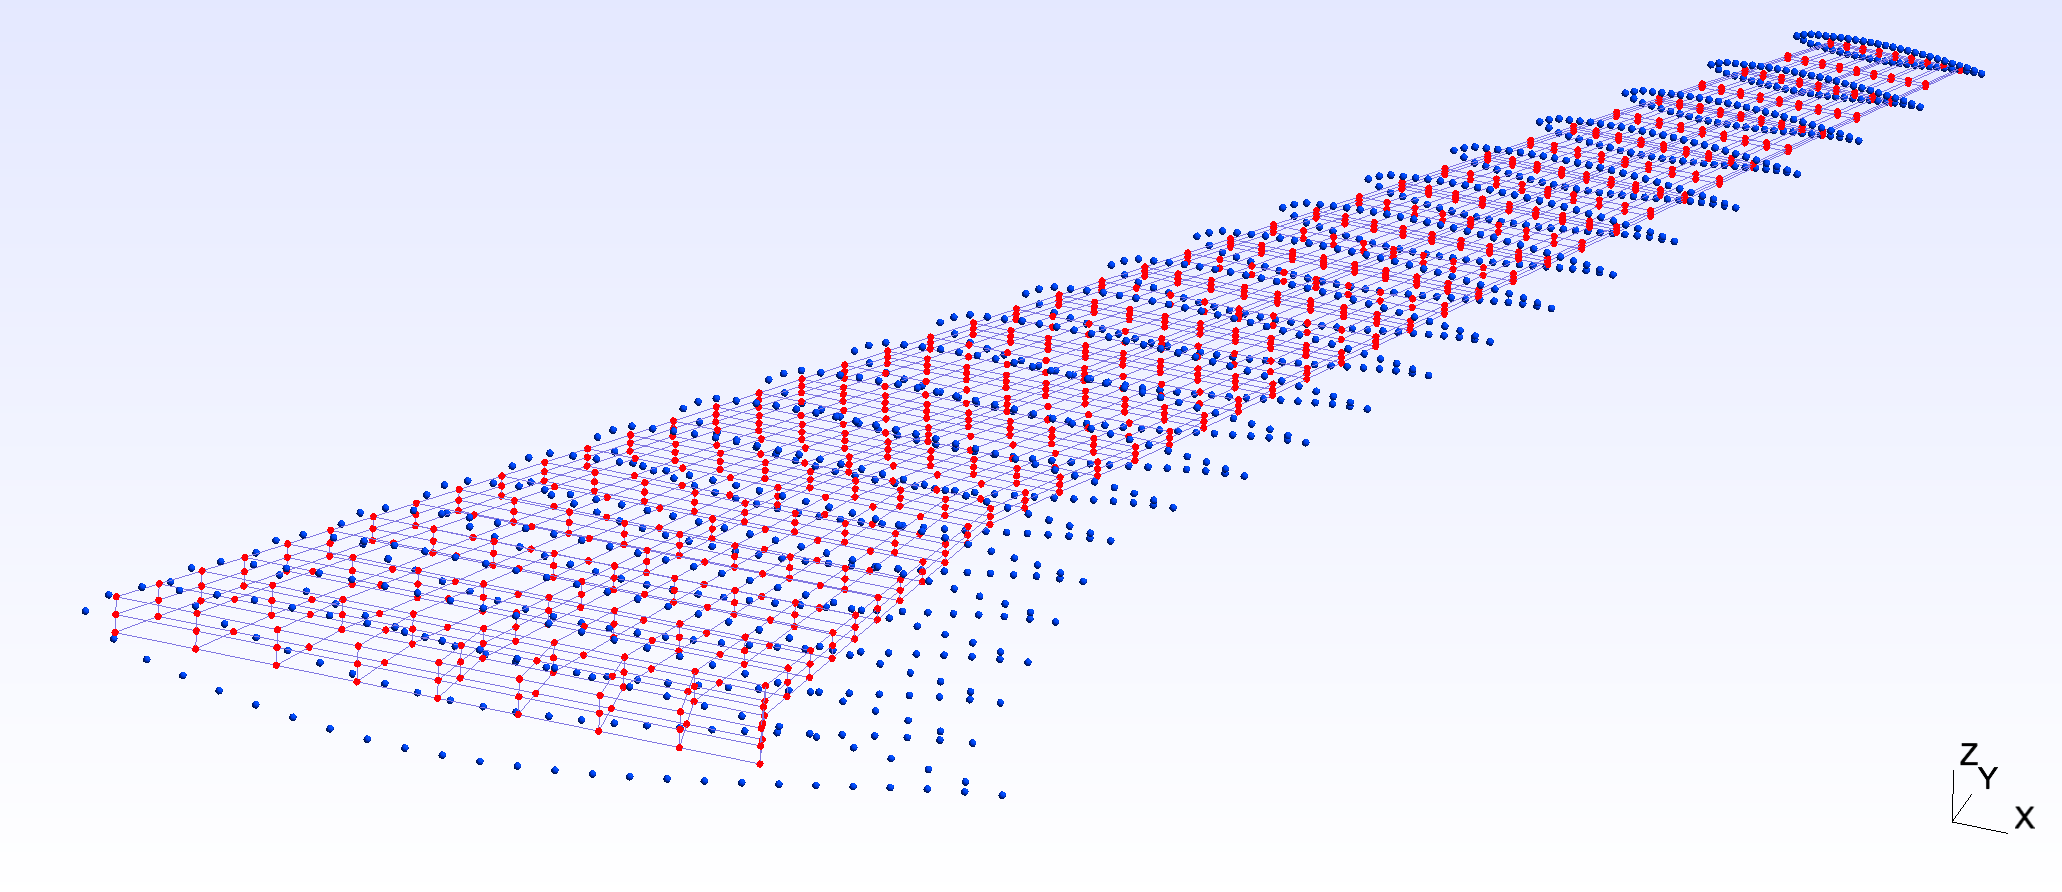
\includegraphics[width = 1\textwidth]{./Immagini/2_3.png}
	\caption{Example of structural mesh (red) and aerodynamic mesh (blue)}
	\label{fig:2_3}
\end{figure}
The input of this component are the outputs of the geometry component, in particular the vector containing the nodes of the CFD mesh $ X_a $ and the vector containing the nodes of the FEM mesh $ X_s $. Instead the output will be the interpolation matrix $ H $. \\This matrix is able to transform the displacements of the structural nodes into displacements of aerodynamic nodes using the formula :
\begin{equation*}
u_a = H \cdot u_s
\end{equation*}
Furthermore, the transpose of this matrix is used to convert the forces of the aerodynamic nodes to the forces of the structural ones with the corresponding formula:
\begin{equation*}
f_s=H^T \cdot f_a
\end{equation*}
\subsection{Aerodynamics}
The aerodynamics component as first creates the shape of the deformed wing by adding the deformation on the initial jig shape, after creates the input file to run an aerodynamic analysis using the external software Panair, than launch Panair, and extracts the aerodynamic characteristics of the wing and stores it into an appropriated dictionary; for each iteration.\\
Once the jig shape is updated, the component creates an auxiliary file that Panin, the input file compiler for Panair, than run Panin in order to get the input file for Panair in a .wgs format.
The aerodynamics loads are computed by means a potential flow panel code, Panair/A502, wich, from an aerodynamic mesh,the value of angle of attack and the Mach, determines the pressure coefficient $C_p$ at the control points of the panel. In order to use the RBF interpolation we need the aerodynamics load on the grid points, so first we use numerical integration of the $C_p$ over the aerodynamic panels and then evenly distributing the total panel forces among the four panel vertexes. A symmetric flow is assumed throughout this work.\\ At the end of process we have a python dictionary which contains the aerodynamics load for each grid point for that iteration.

\subsection{Structure}
The structure component uses the external software Nastran95 to perform the static, and when is request the modal and/or dynamic, analysis of the wing. As first the component takes as input a nastran template file, where is declared the BEGIN BULK section, a sample for each nastran cards used(GRID for nodes, QUAD for shell elements, FORCE1 for the nodal forces, MAT1 for material proprieties,BAR for rod elements \cite{msc}), the mechanical proprieties, the section proprieties, the dictionary containing the coordinates of the structural nodes. Using this parameters the component writes the input files for nastran, where the coordinates of the node from the template file are filled with the dictionary of all structural nodes, and the same for the other nastran card featured in the template file Fig. \ref{fig:2_4}. Until the thickness of the shell elements is assumed as design variables also the thickness vector modified from the optimizer is included in the input variables. Whenever the dynamic analysis is requested it's essential define also the data required for the analysis.\\
When the input file is ready the component launch the nastran software.\\
As for the static structural analysis to compute the displacements of the wing and the stresses of the elements a linear finite element model have been used. The equation that must be solved for the finite element analysis is :
\begin{equation*}
Ku_s=f_s
\end{equation*}
which is linear with respect to the structural displacement, and the stiffness matric $K$ depends only of the material properties and of the underformed geometry, contained in the jig shape. Nastran uses an $LU$ decomposition of the stiffness matrix $K$ to solve the linear system. So seen as structured the problem the $LU$ decomposition of $K$ doesn't change until the optimization process, than it will be stored, and using a $DMAP$ alteration of the FORTRAN code, it will used at the beginning of each MDA loop, to award a computational cost reduction.\\
After the analysis is finished the component takes from the output file (.out for displacement, .pnh for stresses, modal shape, frequencies,$V-g$ and $f-g$ diagrams) the value of the required variables and stores it into an dedicated python dictionary. Nastran can be used also to determinate the mass of the wing, that is an important information, especially when mass is used as objective function. As we will see more detailed in the next chapter, this component can be modified also to extract the mass and inertia properties of a section of the wing, using the nastran weight generator instrument and a unitary load ad nodal forces.
\begin{figure}[H]
	\centering
	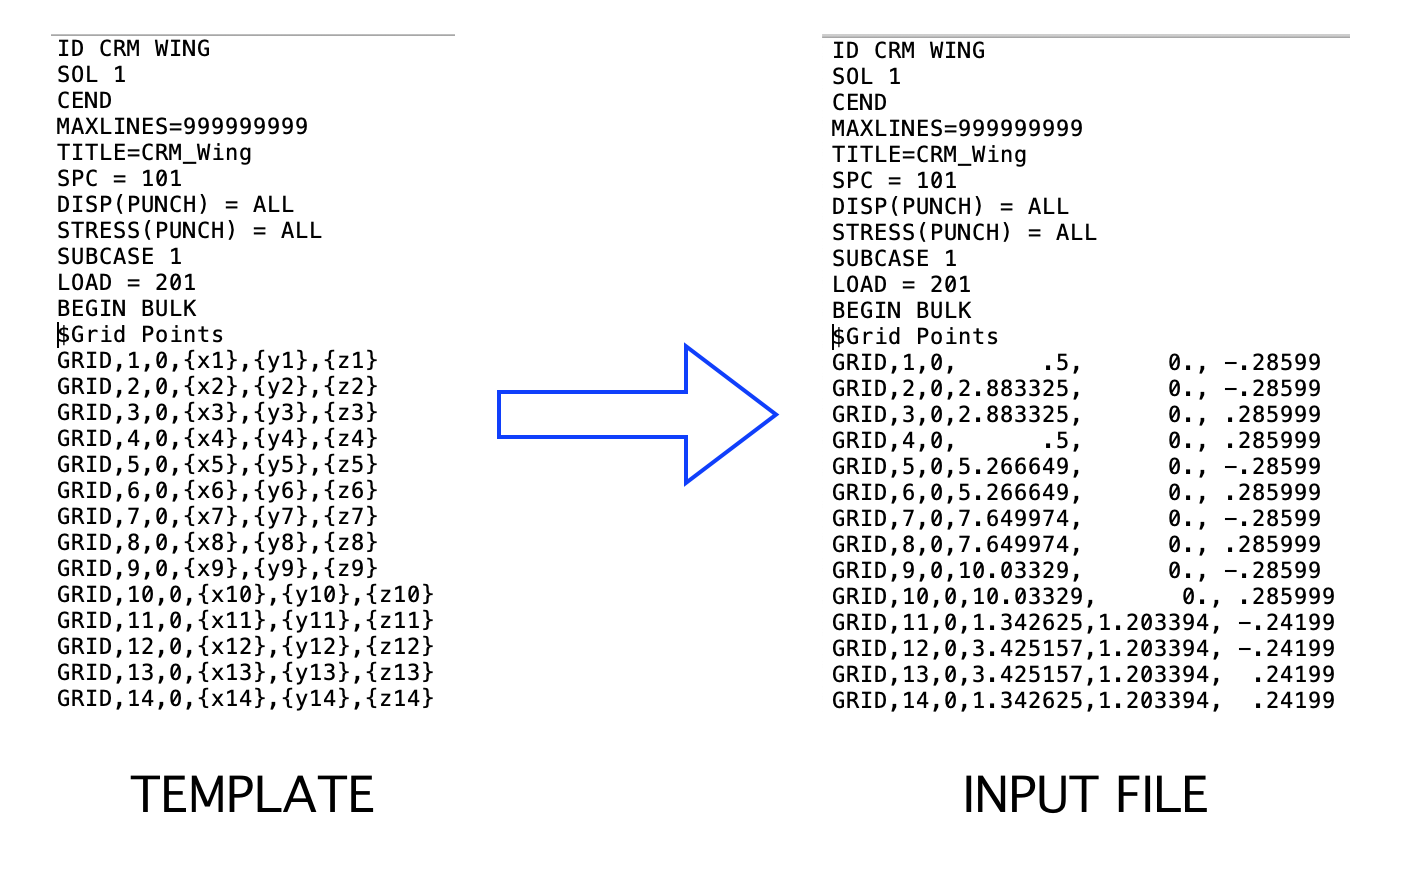
\includegraphics[width = 0.8\textwidth]{./Immagini/2_4.png}
	\caption{Example of nastran template file and input file generated from it}
	\label{fig:2_4}
\end{figure}
\subsection{Load and Displacements Transfer}
In the MDA loop as we said there is coupling between aerodynamic mesh point displacements $u_a$, structural node displacement $u_s$, aerodynamic forces referred on the structural nodes $f_s$ and aerodynamic forces referred on the aerodynamic mesh points.\\
If the aerodynamic mesh is different from the structural mesh it's necessary to interpolate the structural displacement into the aerodynamic mesh points. The displacement interpolation scheme  is based on the work by Rendall and Allen. \cite{all} In that method, each component of the displacement vector \textbf{u} is interpolated as follows (Eq. 2.1 is written for the x component, but the same holds for y and z):
\begin{equation}
u_x=\sum_{i=1}^{N_s}\alpha_i^x\Phi\left(\vert\vert \mathbf{x}-\mathbf{x_i}\vert \vert\right)+\gamma_0^x+\gamma_x^x x+\gamma_y^x y + \gamma_z^x z 
\end{equation}
where $\Phi(r)$ is the form of function adopted. In that case, we choose $\Phi(r)=r^2\ln r$, known as the Thin Plate Spline function (TPS).\cite{joan} According to Lombardi et al. \cite{lomb} who performed a comparison between several available functions, the use of TPS functions is the best and safest option in terms of accuracy of the interpolation. The terms $\alpha_i^x$ are the coefficients of the radial basis functions. Each structural node is the center of an $RBF (\mathbf{x_i})$ and the $\gamma$ terms are the coefficients of the linear polynomial part. By imposing the interpolating condition on these coefficients (the interpolation function evaluated at the structural nodes must be equal to their known displacements) and by evaluating this same function on the aerodynamic grid points, the transformation matrix between the displacements of the structural and aerodynamic points can be expressed as: 
\begin{equation}
u_a=H u_s
\end{equation}
where H is a matrix which depends only on the coordinates of the structural and aerodynamic grid points and the type of RBF chosen.\\
As detailed by Rendall and Allen,\cite{all} and by virtue of the principle of virtual work to ensure the conservation of energy, we can determine the transformation matrix between the aerodynamic forces on the aerodynamic $f_a$ and structural $f_s$ points. The virtual work can be written as:
\begin{equation}
	\delta W = \delta u_s^T \cdot f_s = \delta u_a^T \cdot f_a
\end{equation}
where $\delta u_s$ and $\delta u_a$ are the virtual displacements of the structural and aerodynamic grids respectively. Through the displacement interpolation matrix $H$, we can express the virtual displacements of the aerodynamic grid:
\begin{equation}
\delta u_a=H\delta u_s
\end{equation}
as function of $\delta u_s$. By substituting equation 2.4 into equation 2.3 we get that:
\begin{equation}
	f_s=H^T f_a
\end{equation}
In the case where gradient-based optimization techniques are used for optimization problems that use the aerostructural coupling presented herein, it can be useful to compute the partial derivatives of the coordinates of the deformed aerodynamic mesh $X_a$ with respect to the structural displacements $u_S$, as well as the partial derivatives of the aerodynamic forces on the structural nodes $f_s$ with respect to the forces on the aerodynamic grid points $f_a$.\cite{joan}\\
The deformed aerodynamic mesh is obtained by adding the interpolated displacements (given by equation 2.3) to the jig shape aerodynamic mesh:
\begin{equation}
	X_a=X_a^0+u_a=X_0+Hu_s
\end{equation}
\section{Driver}
In this section is explained how the driver of the problem, the optimization and the aeroelastic coupling driver, is structured. The entirely code is based on the openMDAO structure, so we use  the integrated optimization driver for the optimization loop, and also the integrated equation solver for the aeroelastic coupling loop. Let's see in details how each driver works.
\subsection{Global Optimizer}
The global optimizer controls all the process, it will change the design variables in order to minimize the objective function, each time the design variables change it will launch the mda loop until convergence to determinate the correct aerodynamics loads and structural displacement, and consequently the right stresses, after that it will check if the constraint is respected and the effect of the changes on the objective function, than it will repeat this process until convergence. \\
To define the optimization driver first thing is to choose the optimizer and set the optimizer option, after need to define the objective function, the constraint and the design variables.
\subsubsection{Optimizer}
The optimizer chosen for this problem are two:
\begin{itemize}
	\item \textbf{COBYLA}: a gradient free optimizer
	\item \textbf{SLSQP}: a gradient based optimizer ( in this case gradient will be calculated using finite differences method)
\end{itemize}
In the examples chapter optimization using both method on the same model have done, to see the differences between the two optimization method.
\subsubsection{Design Variables}
In this code several design variables were implemented:
\renewcommand{\labelitemi}{--}
\begin{itemize}
\item The angle of attack $\alpha$
\item The twist angle $\theta$
\item The mid spar position
\item The scale factor
\item The area of stringer
\item The sweep angle $\Lambda$
\item The cord factor
\item The thicknesses of the different section of the wing inputted as an array *
\end{itemize}
* The structural design variables consist of the thicknesses of the structural finite elements. The topology of structure remains unchanged. In the FEM model we divided the QUAD elements in groups, all the elements of the same group has the same thickness. How you can see in Fig. \ref{fig:2_5} there are different group for the upper surface and for the longerons, so we collect all the information about the thickness in an array. During the optimization process the thicknesses array can be set as design variable.
\begin{figure}[H]
	\centering
	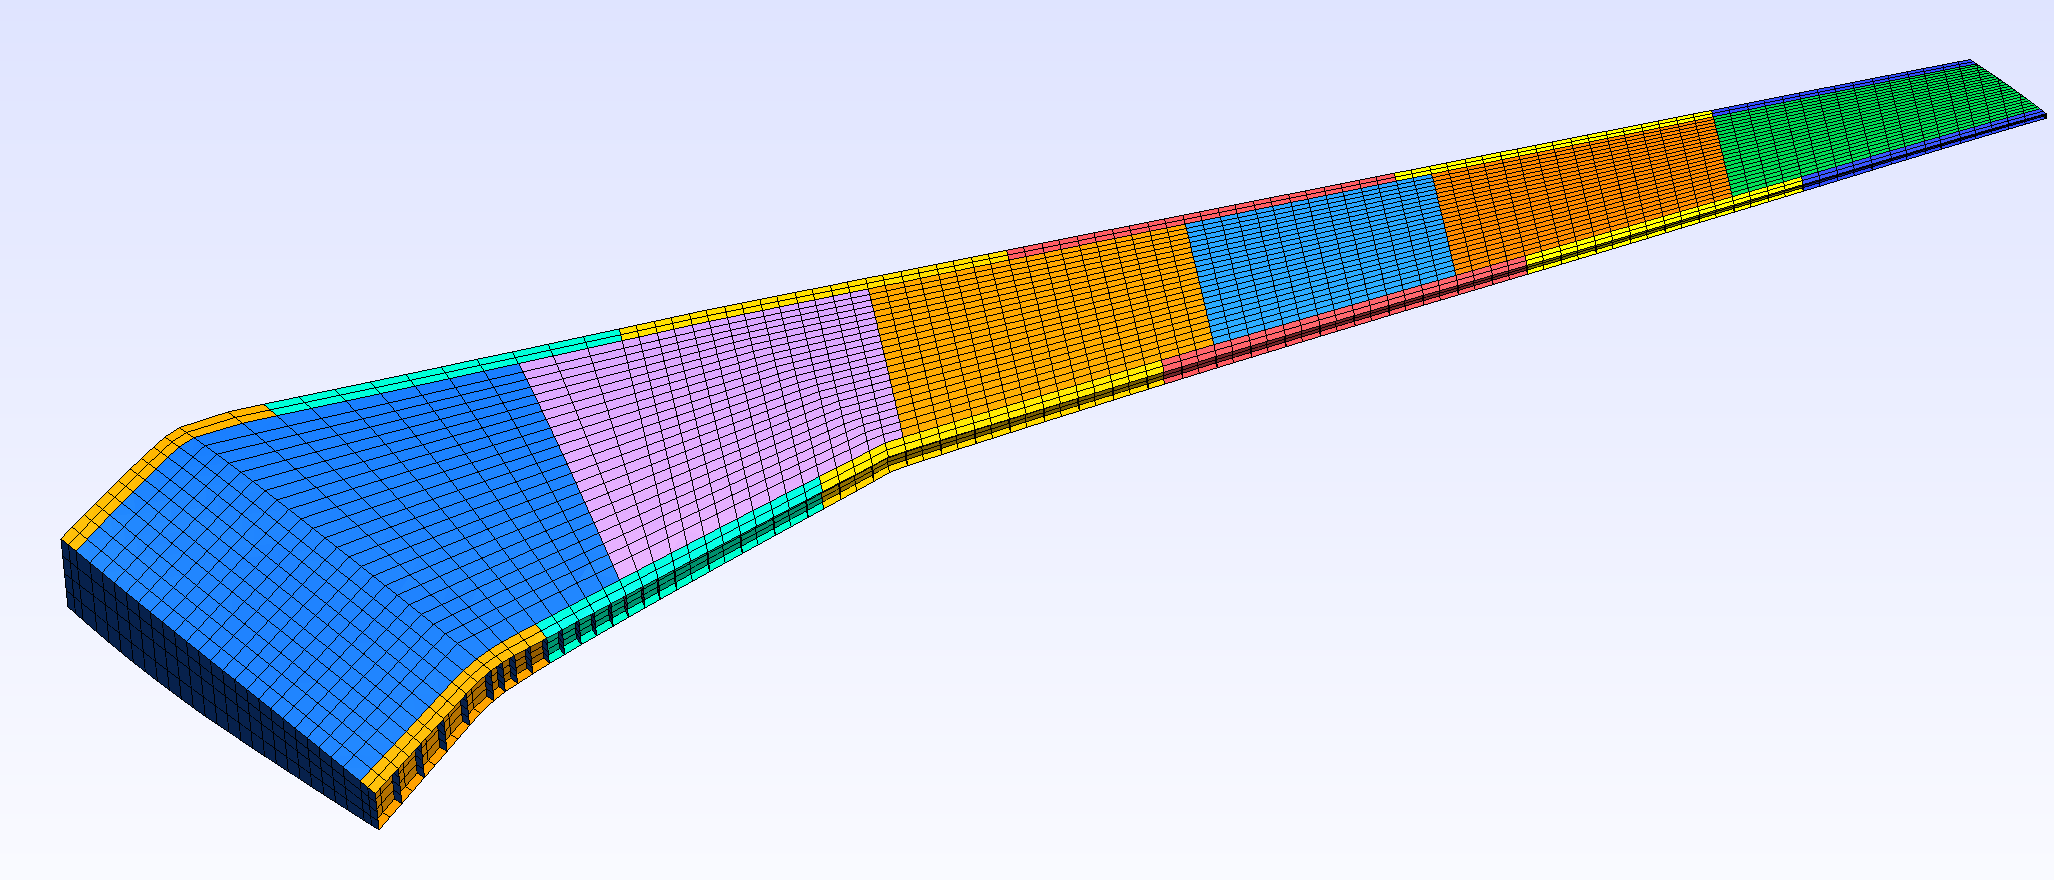
\includegraphics[width = 1\textwidth]{./Immagini/2_5.png}
	\caption{Different thickness sections in the CRM FEM model}
	\label{fig:2_5}
\end{figure}
For each design variable it's possible to set the limits and the initial value. It's possible also to choose just one, a group or all the design variables. In fact in the test cases presented in this work, where the relevant aspect is to test the aggregation component just the angle of attack and the thickness vector is selected as design variables, while all the variables related to the geometry are assumed as constant, so once the geometry is defined it will not change until the process.
\subsubsection{Constraint}
As for the constraints that were imposed, there is one constraint concerning the lift, where the lift must be at least equal to the weight of the aircraft during the cruise, we constrain the $C_L$ by periodically adjusting of the angle of attack of the aircraft within the aero-structural solution until the desired lift is obtained; to set a constraint like this it's necessry to define an \textit{Executable Component}, a component of openMDAO where it's possibile to define a function that is updated for each iteration, and after set this function as constraint imposing the lower or the upper limit. \\In this case the constraint will be:
\begin{equation*}
	C_L - \frac{2W}{\rho_aV^2S_w }> 0
\end{equation*}
The stresses is also considered, so in addition to maintaining the $C_L$ there is also a stress constraint that guarantee the stress of material is lower of the yield stress at the various load condition. The stresses is the result of the structural analysis performed with the finite elements method, so it's necessary to check that the stress of each element respect the constraint, to do this it's necessary to create an \textit{Executable Component} for each element, but usually over than thousand od elements is necessary to describe the structure of the wing, and it becomes computationally very costly to treat these constraints separately. To avoid this problem in the next chapter is explained how we implemented the constraint aggregation.\\ In this case the constraint will be:
\begin{equation*}
\sigma_i - \sigma_{yield} < 0 \ \ \ \ for \ \ \ \ i=1,2,...,N_e
\end{equation*}
where $N_e$ it's the number of finite elements.

\subsubsection{Objective Function}
In the typical aircraft optimization problem the objective is to find the good trade-off between aerodynamic drag and structural weight. So for our optimization problem we set as objective function the induced drag coefficient $C_{D_i}$ and the structural mass $W$, or in the general case a function like:
\begin{equation*}
F = \alpha C_{D_i} + \beta W
\end{equation*}
where $\alpha$ and $\beta$ are scalar parameters that is indicative of the relative importance of the variables that we want to minimize.\\
Is important note that openMDAO is able to manage just minimization problem, so to manage maximization problem is necessary to create an objective function equal to the negative of the real objective function.
\subsection{MDA Driver}
To solve the coupling problem between aerodynamics loads and structural displacements it's necessary an internal loop that through an iterative process which update iteration for iteration the value of the variables implicitly linked reach the convergence. That process is tasked to a non linear equation solver, in this case we choose one of the solver included in the openMDAO library, the non linear Gauss Seidel Solver \textit{NLGaussSeidel} with the aitken accelaration \cite{ait}.\\
To do this the MDA driver call the components that we discussed above in order to reach the convergence. In the Fig. \ref{fig:2_6} it's showed the XDSM concerning the MDA loop: 
\begin{figure}[H]
	\centering
	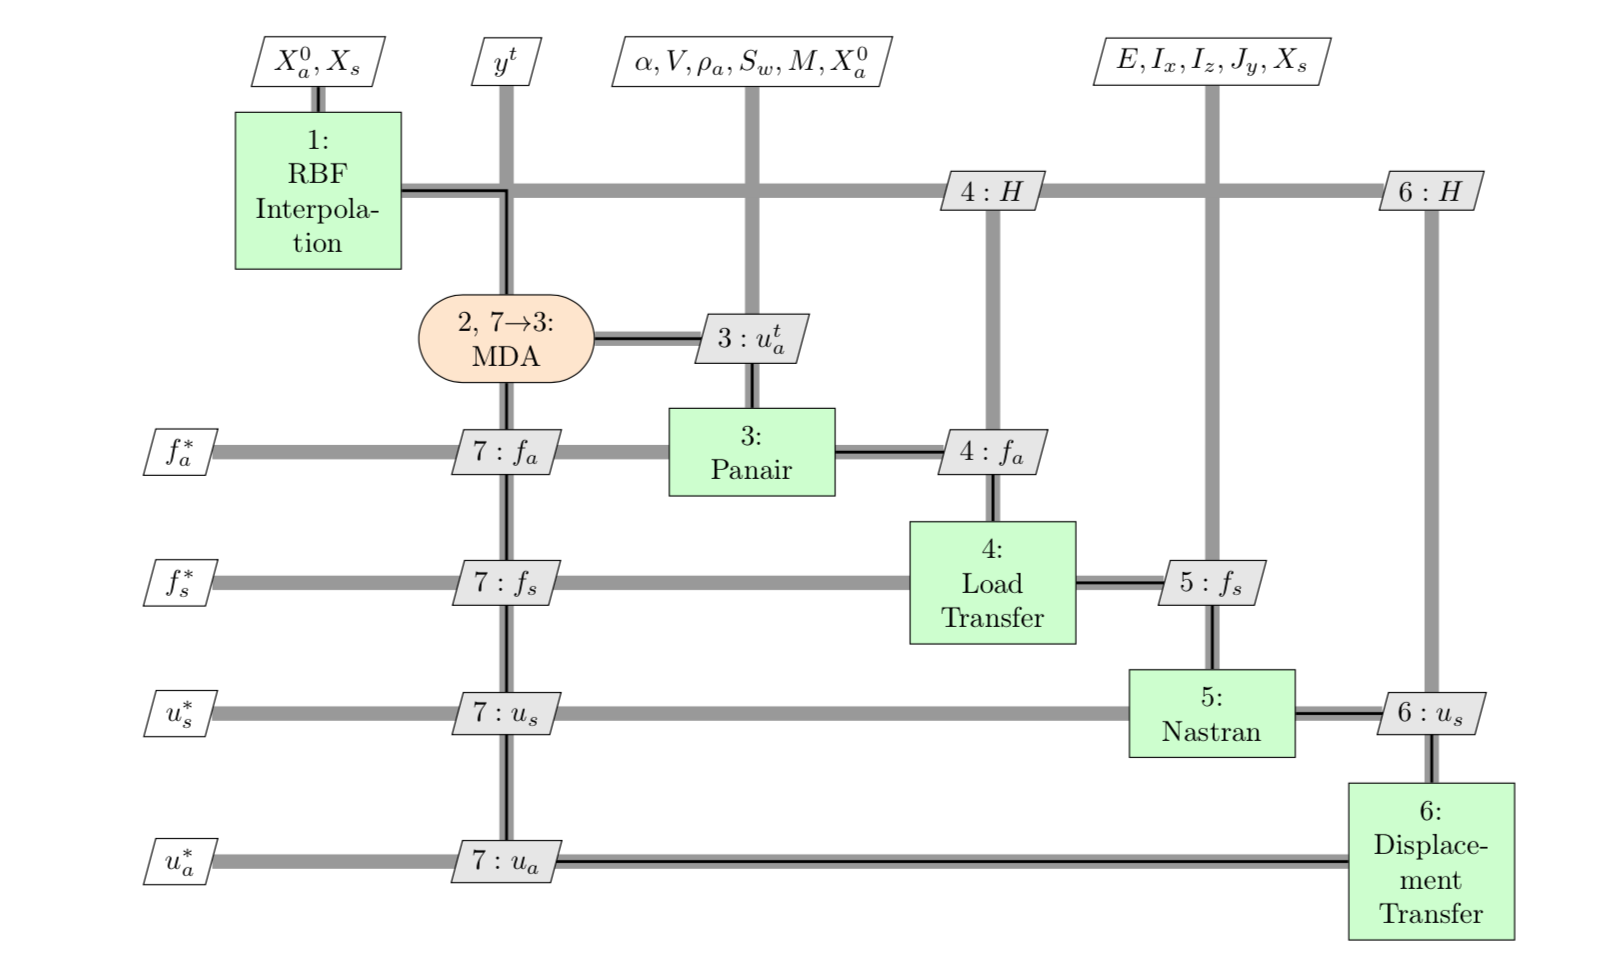
\includegraphics[width = 0.8\textwidth]{./Immagini/2_6.png}
	\caption{XDSM of the MDA Driver}
	\label{fig:2_6}
\end{figure}
The required parameters for each component is the following, fro:
\begin{itemize}
	\item RBF interpolation: the aerodynamic mesh $X_a^0$ and the structural mesh $X_s$;
	\item Aerodynamic analysis: the angle of attack $\alpha$,the flight speed $V$, the density of the air $\rho_a$, the wing surface $S_w$, the Mach $M$;
	\item Structural analysis: the Young module $E$,the barycentric moment of inertia $I_x,\ I_y \ and\  I_z$;
\item Interpolation: the interpolation matrix $H$.
\end{itemize}
	while the coupling variables are $u_a,\ u_s,\ f_a\  and\  f_s$.
The steps to reach the coupling convergence is the following:
\begin{enumerate}
	\item Compute the interpolation matrix $H$.
	\item Initiate the MDA loop.
	\item Compute the aerodynamic forces on the aerodynamic grid points.
	\item Compute the aerodynamic forces on the structural grid points.
	\item Compute the structural displacements.
	\item Compute the aerodynamic grid point displacements
\end{enumerate}
Repeat $3\rightarrow 7$ until convergence.
In Fig. \ref{fig:2_7} it's showed how the vertical displacement of the wingtip nodes change until the process, and how the MDA loop reach the convergence. 
\begin{figure}[H]
	\centering
	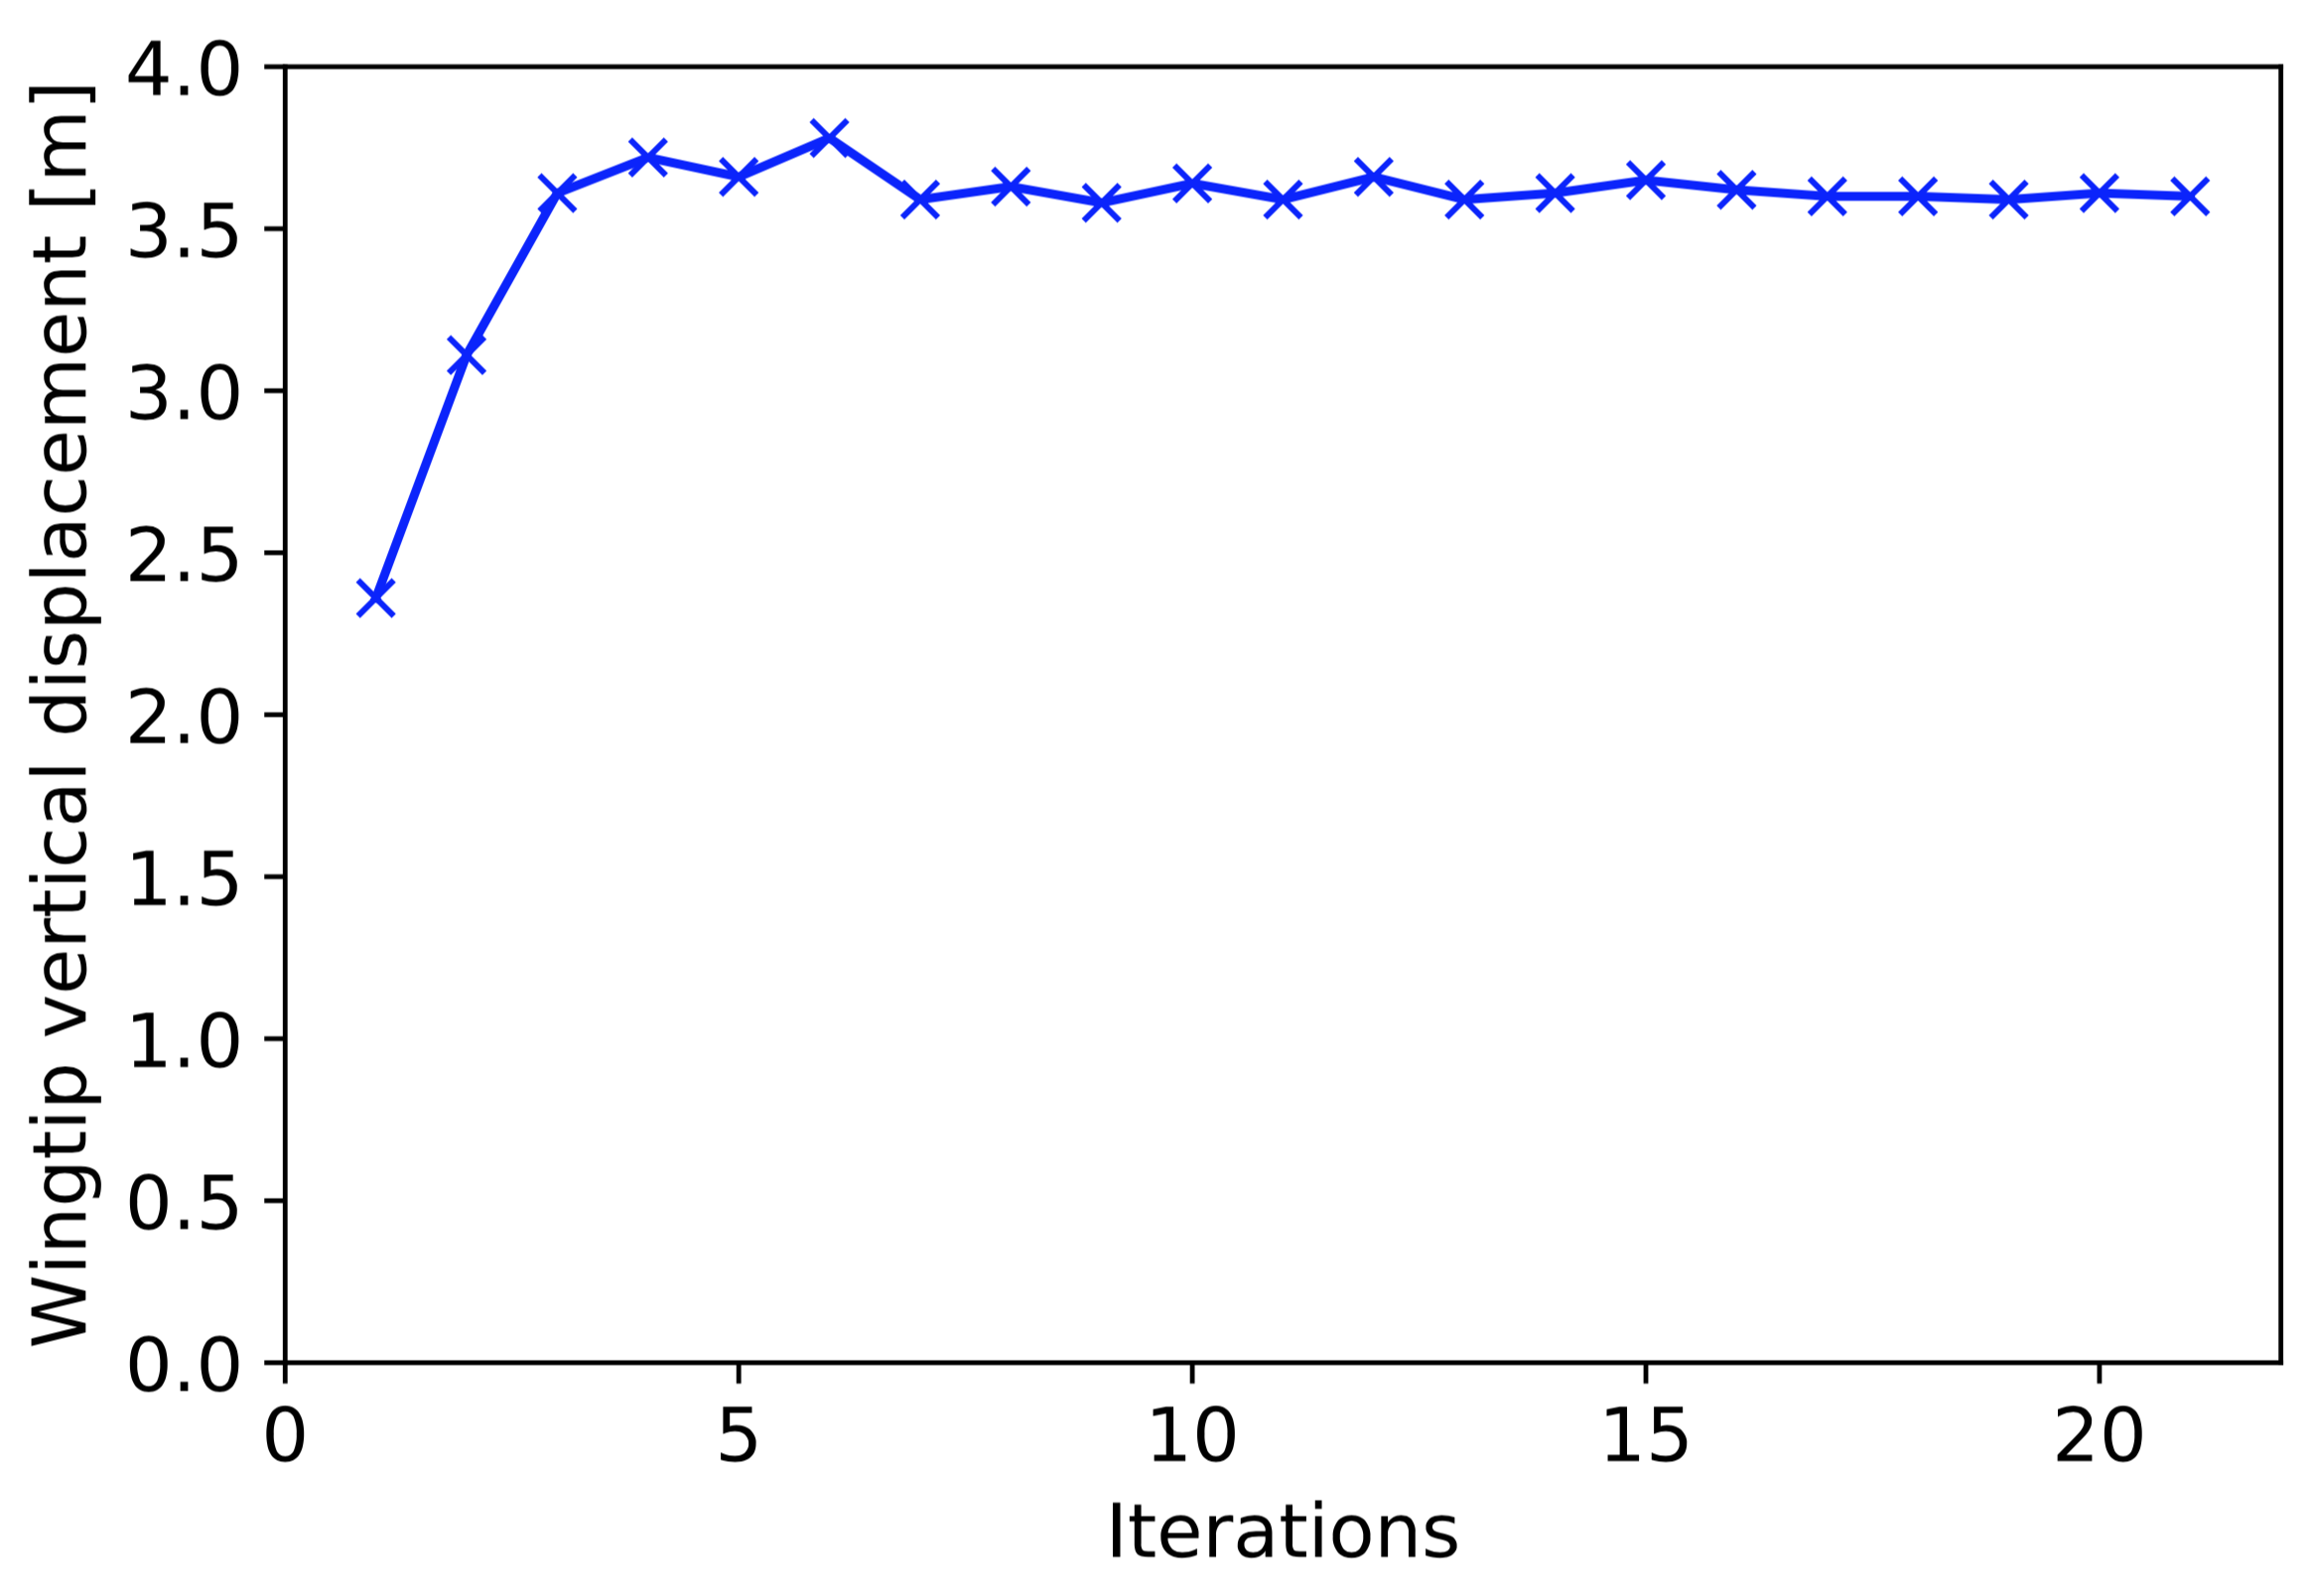
\includegraphics[width = 0.8\textwidth]{./Immagini/2_7.png}
	\caption{Results of the MDA loop refered to the wingtip vertical displacement }
	\label{fig:2_7}
\end{figure}
For each optimization iteration, the MDA loop determinate the displacements and the aerodynamic loading considering the aeroelastic coupling. Normally to reach the convergence needs 6 or 7 iteration, for each iteration one aerodynamic analysis and one static structural analysis is performed, so for high fidelity model, aerodynamic and/or structural, the computational cost can be huge, that's the first reason to introduce a reduce model for the MDA loop, showed in the chapter 4.
%
\chapter{Constraint Aggregation} 
\label{chapter3}
\section{Aggregation}
For aircraft wing design, currently, there is a trend to employ higher-fidelity (more expensive) and multidisciplinary numerical simulations, such as the coupling of CFD code and CSD code. In addition, optimization problems become more and more complex, with many design variables, tightly coupled objectives, and a large number of constraints. Handling large-scale constraints presents a challenge for wing structural and aero-structural design, since the refined finite element model with multiple freedoms incurs millions of structural failure constraints. \cite{zha}\\
In our optimization problem we are also interested to minimize the structural mass subject to constraint on structural failure, in particular we are interested in failure based on yield stress. In the design checking the failure criteria in the optimization process is desirable, because allow to verify that the optimized structure is suitable for the prescribed load conditions.\\
The primary issue with including failure constraints directly in the structural optimization problem is the resulting size of the optimization problem. Conceptually, for a continuum structure, failure constraints need to be enforced throughout the material domain, leading to an infinite number of constraints. More practically, failure constraints may be enforced element-wise in the finite element model. For detailed, high-fidelity structural models, this can lead to an optimization problem with many thousands or millions of failure constraints. These constraints are costly to enforce because they can only be checked by completing the structural analysis.\cite{lambe}\\
Aggregation methods allow to manage an huge number of constraints, in fact that methods lump a large number of constraint into one global constraint, so the computational cost of the multidisciplinary optimization drastically decrease. These methods consist in the use of an aggregation function, which transform a set of local function values into a scalar function. This scalar function converge in the limit to the maximum local function value:
\begin{equation*}
\lim_{P\to\infty} G(\mathbf{f},P)=\max(f_1,f_2,...,f_N)
\end{equation*}
where $\mathbf{f}$ = $(f_1,f_2,...,f_N)^T$ is a vector in which the entries are the local function values, $G$ is the scalar aggregation function and $P$ is the draw-down factor that manage the aggregation.\\
There are different aggregation function, some of them approximate the maximum of the local function from above, and other from belove. So depending on this characteristic behavior aggregation function forms an upper or lower bound to the maximum local function value.\\
Related to our problem aggregation function became necessary for the stress failure constraints, in fact when the structural model is detailed, so the number of elements became huge, we need to check the stress criteria on each single element; this entails that need one constraint for each element in the optimization process, with the result that the computational cost became prohibitive, and openMDAO find problem in the setup phase to creates this huge number of constraint, and sometimes it can crash in this phase.Additionally using a gradient-based optimizer the aggregation fucntion can avoid the problem of the not differentiable maximum function, increasing the curvature of the function in the region where there is this problem modifying the draw-down factor. That's one of the reason because we implemented a new component in the optimization process, the aggregation component, so the XDSM of the optimization process is modified as follow:
\begin{figure}[H]
	\centering
	\includegraphics[width = 0.8\textwidth]{./Immagini/3_1.png}
	\caption{XDSM after constraints aggregation}
	\label{fig:3_1}
\end{figure}
As we can see after the implementation of the aggregation component a new box function have been added, the box function 11. So after the extraction of the Von Mises stresses vector by the structural component the aggregation component take this vector as input and give as output the scalar $G$. Now the constraint function is connected to$G$ and to $\sigma_{yeild}$, so the constraint will be determinate using these variables.
\subsection{Aggregation Method}
Let's see how the aggregation implementation modifies the approach of the optimization design problem, and in particular referred to our problem. \\
Suppose the original problem is to optimize the mass of a structure under the failure criteria constraint, the problem in this case can be written as:
\begin{align*}
&minimize \qquad \quad m\\
&subject\ to \qquad  \sigma_{VM_i}< \sigma_{Yield}\qquad \forall \ i=1,2,...,N
\end{align*}
where $m$ is the mass of the structure, $\mathbf{\sigma_{VM}} =[\sigma_{VM_1},\sigma_{VM_2},...,\sigma_{VM_N}]$ is the vector containing the Von Mises stresses of each finite element used for the structural analysis, $\sigma_{Yield}$ is the yield stress and $N$ is the number of the finite elements.\\
Let's see how the problem is modified using the maximum constraint approach, the simplest aggregation method. Using this method we have that the most violated constraint is selected, while the rest are ignored. \\In this case the problem can be written as:
\begin{align*}
&minimize \qquad \quad m\\
&subject\ to \qquad  \max (\sigma_{VM_i})< \sigma_{Yield}\qquad  \ i=1,2,...,N
\end{align*}
However, because the constraints is not smooth it's not possible to use a gradient-based algorithms in the optimization process, and the search direction is determined by considering only the Lagrange multipliers of the most violated constraint, usually leading to the violation of another constraint in the next iteration.\\
Using an constraint aggregation function the optimization is subject to the value of the aggregation function $G$, so the problem can be written as:
\begin{align*}
&minimize \qquad \quad m\\
&subject\ to \qquad  G < 0
\end{align*}
where $G$ is a scalar, given from the aggregation function and it's representative of the maximum value of the Von Mises stresses vector. $G$ depends, as we said, also to the aggregation function choose, so in the next paragraph we will introduce the most common aggregation function, and theirs properties.
\section{Aggregation Functions}
In literature several aggregation function have been used. The choice of the function depends of the nature of the problem, of the size of the problem and of the properties required to perform the analysis. For the failure criteria, where the constraint impose the stresses lower than yield stress, the natural choice for these constraint aggregates is a maximum- or minimum-value function. But the problem it's that this kind of functions are not differentiable, so cannot be used efficiently in gradient-based optimization. Another choice can be the \textbf{p-mean} and \textbf{p-norm} function, or the \textbf{Kreisselmeier-Steinhauser KS} function, kind of smooth estimator. These estimators do not precisely reproduce the true feasible design space provided by the original constraints, so the final design determined by the optimizer will be different depending on the aggregation scheme. \cite{lambe} 
\subsection{Function}
First, we briefly discuss aggregation function used in the literature.\\
About the nomenclature we use $G$ to indicate the aggregation function, the superscript $_L$ and $_U$ to denote respectively an lower- or upper-bounded aggregation function, and $P$ to indicate the draw-down factor.\\
The first two aggregation function that we analize is the \textbf{p-norm} and the \textbf{p-mean} function. This kind of aggregation function can be use when the local function value $\mathbf{f}$ are non-negative, as in our case where $\mathbf{f}$ is the Von Mises stresses vector, so for definition we have that all the component of the vector, the Von Mises stress of each finite element, is positive.
\subsubsection{P-norm}
\begin{equation}
G_{PN}^U=\left(\sum_{i=1}^{N}f_i\right)^{1/P}
\end{equation}
\subsubsection{P-mean}
\begin{equation}
G_{PM}^L=\left(\frac{1}{N}\sum_{i=1}^{N}f_i^P\right)^{1/P}
\end{equation}
The difference between these two aggregation functions is that the P-norm is an upper bound, and the P-mean is a lower bound to the maximum local function value:
\begin{equation*}
G_{PM}^L \le \max(f_1,f_2,...,f_N)\le G_{PN}^U
\end{equation*}
For this propriety it's important to note, in the implementation in an optimization process, that the p-norm function is conservative, backwards the p-mean is not conservative.
\subsubsection{Kreisselmeier-Steinhsauser function}
The Kreisselmeier-Steinhsauser aggregation function have been presented for the first time by G. Kreisselmeier and R. Steinhsauser \cite{krei}.The function constains a “draw-down” factor or aggregation parameter, $P$, which is analogous to the penalty factor in penalty methods used to perform constrained optimization \cite{poon2}.\\
This function have been used first to aggregate multiple objectives and constraints into single functions, but in the time became popular to be used in the direct constrained optimization problem. This function has few important proprieties, about we will discuss after, but ne of the more important property is the following: "The function produces an envelope surface that is $C1$ continuous and represents a conservative estimate of the maximum among the set of functions" \cite{nasa}.\\
The KS function can be used also to aggregate only the constraints into a single continuous function, in that way is defined as:
\begin{equation}
G_{KS}^U=\frac{1}{P}\ln\left(\sum_{i=1}^{N}e^{Pf_i}\right)
\end{equation}
This function, as the superscript denote, is an upper bounded function, for each $P>0$, so it overestimates the maximum local function value. Let's see the properties of this function:
\begin{align*}
G_{KS}(x,P)\ge\max(f_i(x))                     &\qquad for \qquad P>0\\
\lim_{P\to\infty}G_{KS}(x,P)=\max(f_i(x))& \qquad for \qquad j=1,2,...,N\\
G_{KS}(x,P_1)\ge G_{KS}(x,P_2)             &\qquad for\qquad  P_1>P_2>0\\
G_{KS}(x,P) \qquad\qquad                     &\qquad is\ convex,\  if\  and\  only\  all\  constraint\  are\  convex
\end{align*}
These properties is really important for the KS function to be considered an valid aggregation function. The first three properties indicate, as we said, that the KS function is upper-bounded, it overestimates the maximum of the constraint defined as $G_i\le0$, a positive value returned indicate that a constraint is violated or close to being violated. The conservative nature is determined from the aggregation parameter $P$, id $P$ increases the aggregation function value became more closer to the maximum value. The effect of the aggregation parameter will be investigate in the next paragraph, but in Fig. \ref{fig:3_2} we can see that effect from the investigation done by J. R. R. A. Martins, for a two constraints problem, $g_1$ and $g_2$: \cite{poon2}:
\begin{figure}[H]
	\centering
	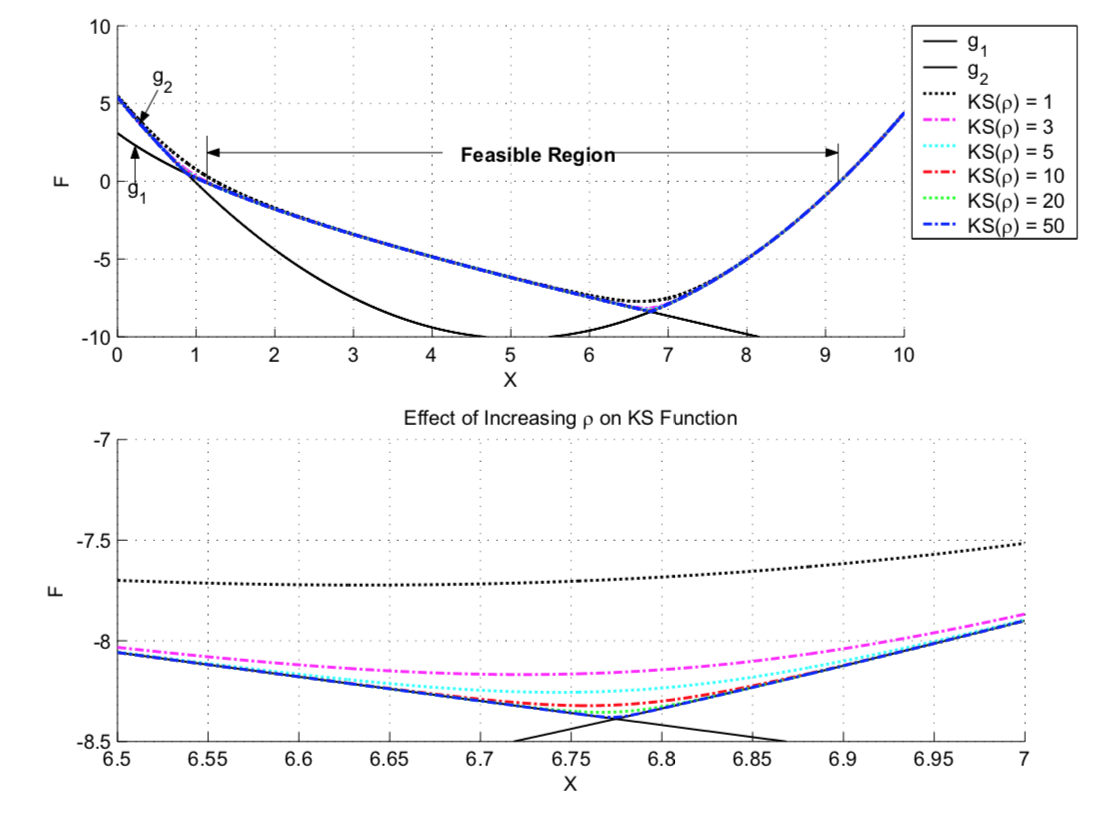
\includegraphics[width = 0.8\textwidth]{./Immagini/3_2.png}
	\caption{Effects of the aggregation parameter $P$ on the KS function}
	\label{fig:3_2}
\end{figure}
An alternative formulation can be used, to avoid numerical difficulties caused by numerical overflow, the KS function can be written as:
\begin{equation}
G_{KS}^U=f_{max}+\frac{1}{P}\ln\bigl[\sum_{i=1}^{N}e^{P(f_i-f_{max})}\bigr]
\end{equation}
where $f_{max}$ is the max value of the local function.\\
The maximum difference between the maximum value of the local function and the value of the aggregation function is determinate by $P$, and it's value its:
\begin{equation}
\frac{1}{P}\ln\left(Ne^{Pf_{ma}}\right)-f_{max}=\frac{1}{P}ln(N)
\end{equation}
that's mean:
\begin{equation}
f_{max}<G_{KS}<f_{max}+\frac{1}{P}ln(N)
\end{equation}
From this property can be obtained an alternative formulation of the KS function, a lower bounded KS function. To obtain it we need to subtract the maximum difference between the maximum of the local function to the KS upper bounded function, obtaining :
\begin{equation}
G_{KS}^L=G_{KS}^U-\frac{1}{P}ln(N)=\frac{1}{P}ln\left(\frac{1}{N}\sum_{i=1}^{N}e^{Pf_i}\right)
\end{equation}
that became the following using the alternative formulation:
\begin{equation}
G_{KS}^L=f_{max}+\frac{1}{P}\ln\bigl[\sum_{i=1}^{N}e^{P(f_i-f_{max})}\bigr]-\frac{1}{P}ln(N)
\end{equation}
\subsection{Effects of the Aggregation Parameter $P$}
The aggregation parameter or draw-down factor $P$ has several effects on the aggregation function. Choose it correctly is really important to have low relative error of aggregation function relatively at the real maximum of the local function, and also a low computational cost. The right choice of the aggregation parameter depends as first of the problem size, but also from the dispersion of the value of the local function and their absolute value. In addiction is important to choose the draw-down factor to smooth the aggregation function in the region where the constraints intersect, to be possible to compute the derivatives.\\
As first we can see in Fig. \ref{fig:3_3} how the size of the problem influence the relative error for a given draw-down factor. We use the aggregation function to aggregate the Von Mises stresses vector, so the value of the aggregation function is representative of the maximum stress for the finite elements of the structure. In this case we choose a Kreisselmeier-Steinhsauser function lower bounded, we set the draw-down factor as 50, then we compute the relative error as:
\begin{equation*}
\epsilon = \left| \frac{G_{KS}^L-f_{max}}{f_{max}} \right|
\end{equation*}
Than we compute the relative error for different size of the stresses vector. Locking the draw-down factor we can see how the relative error grow with the size of the problem, or analogously with the number of the constraints that we want to aggregate.
\begin{figure}[H]
	\centering
	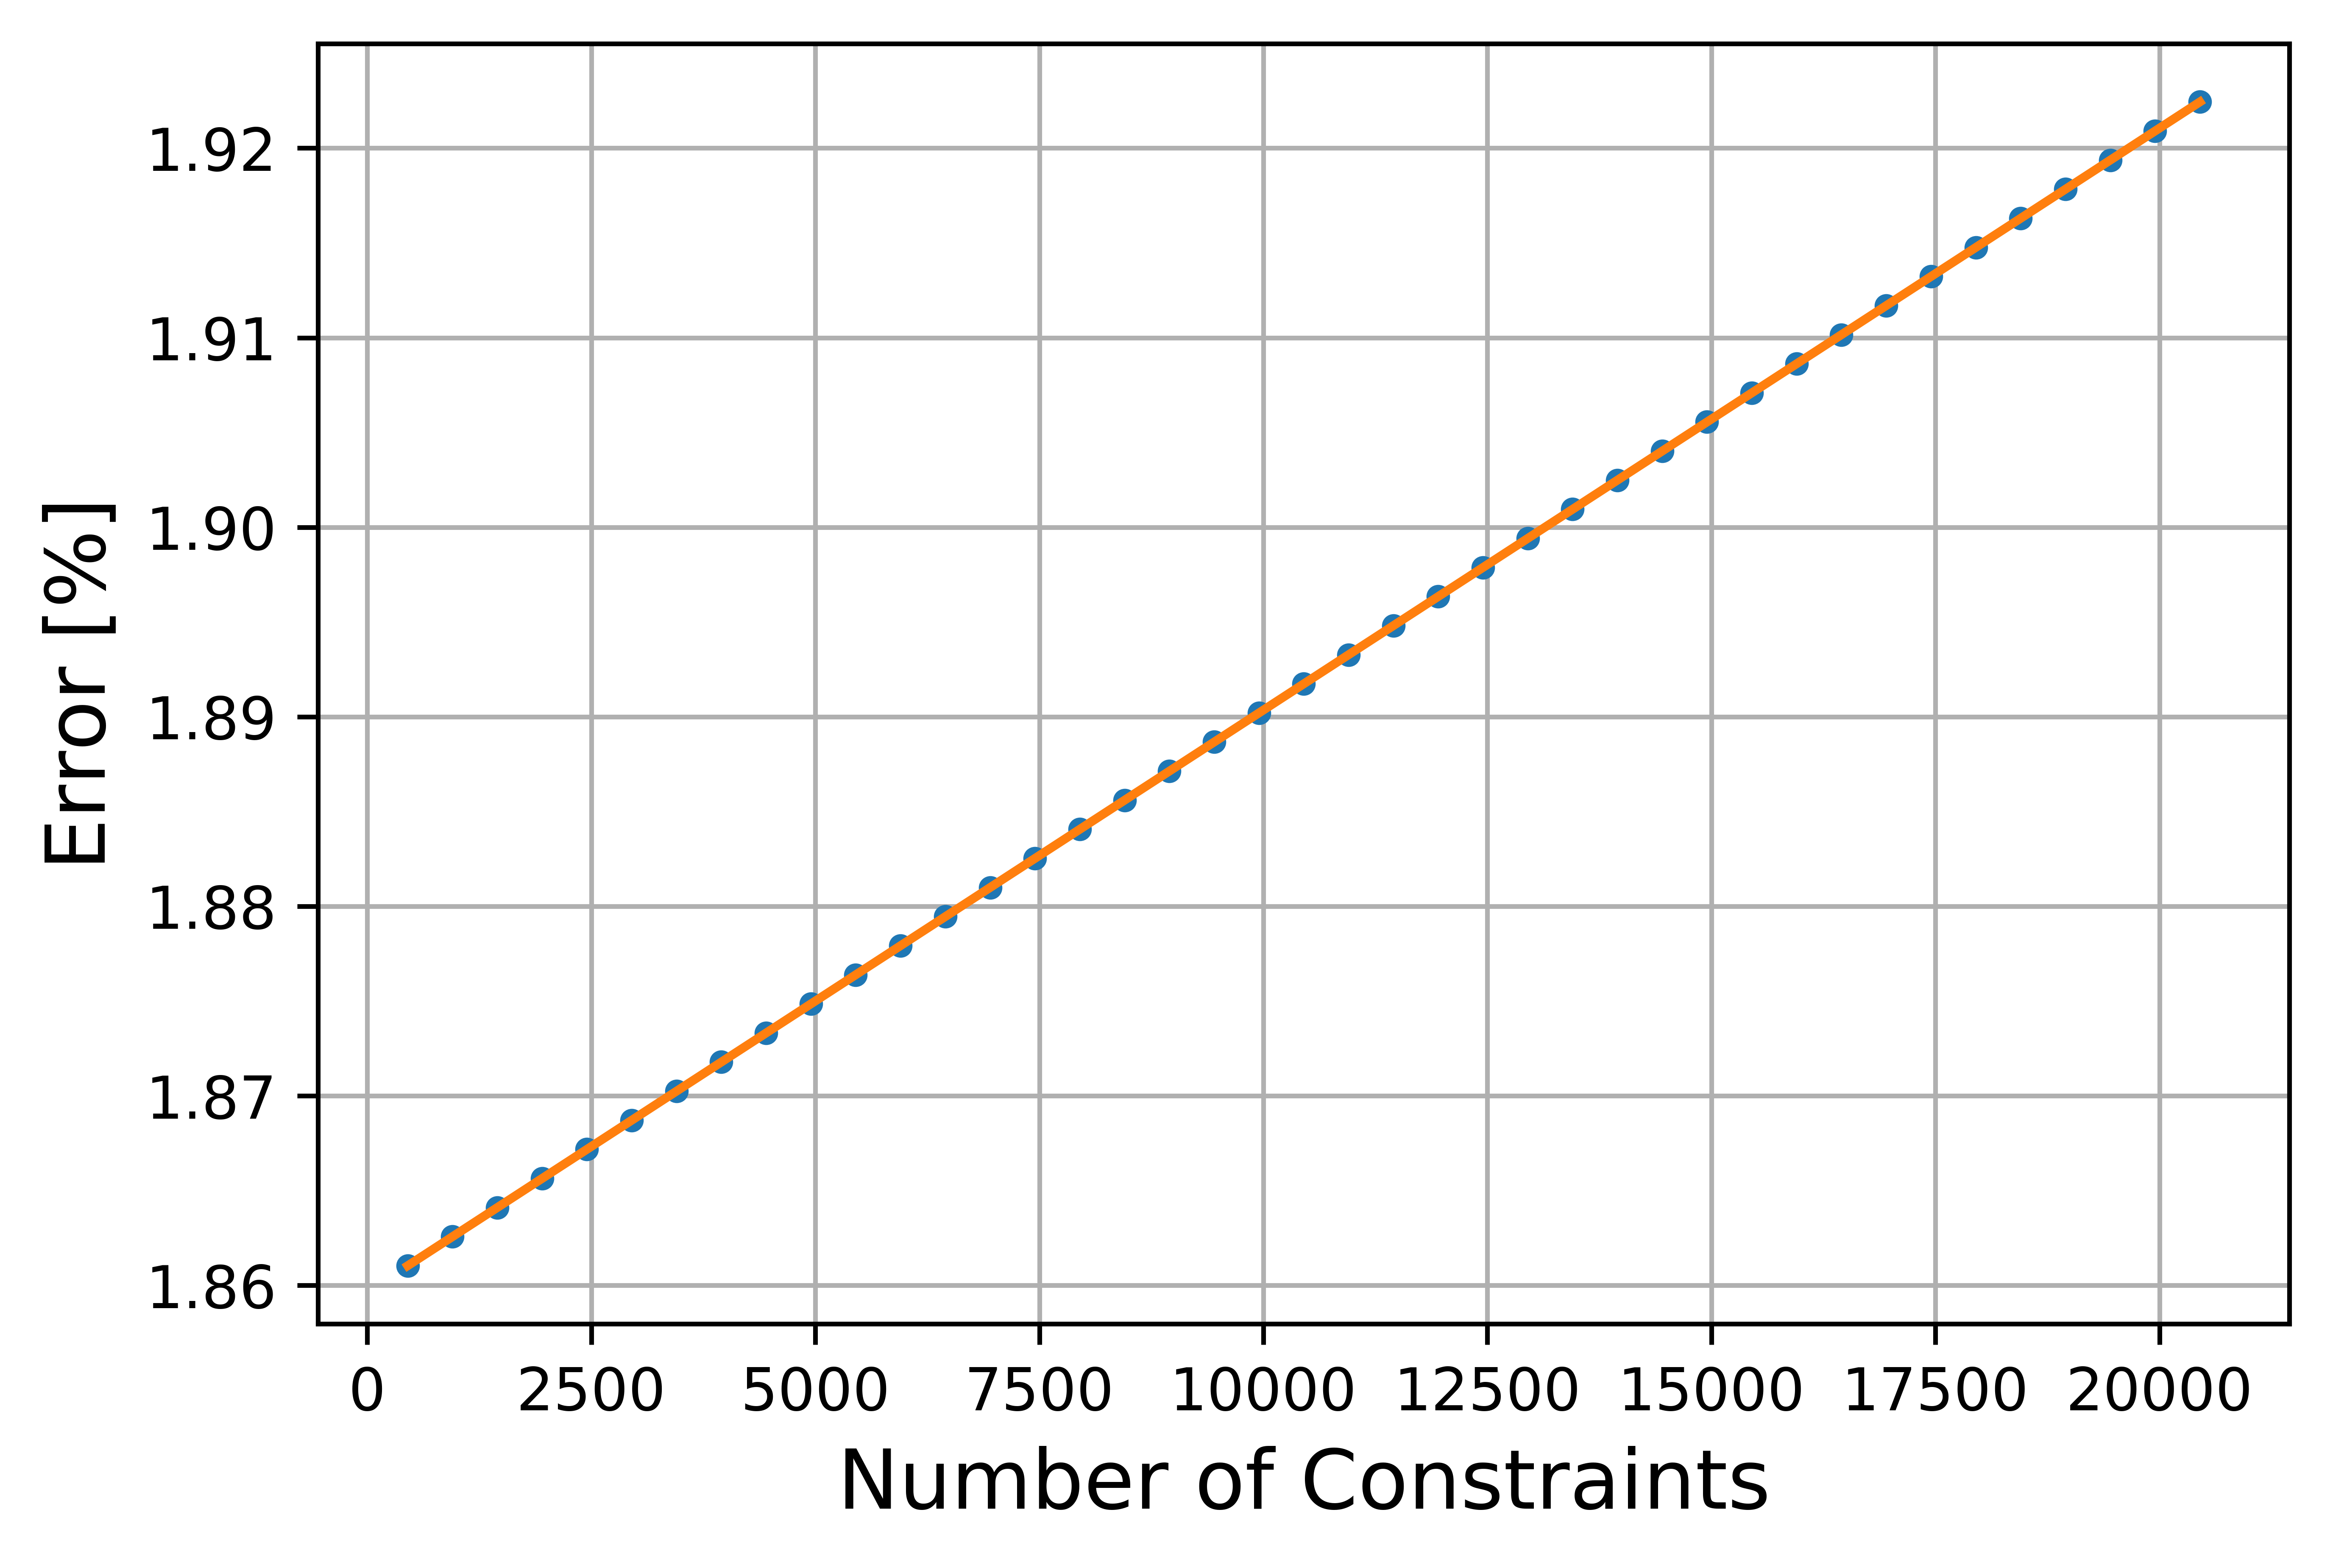
\includegraphics[width = 0.8\textwidth]{./Immagini/3_3.png}
	\caption{Effects of the number of constraint on the relative error of the aggregation function}
	\label{fig:3_3}
\end{figure}
The choice of aggregation parameter is also constrained to the aggregation function and to the maximum relative error. In Fig. \ref{fig:3_4} there are showed how the relative error changes with the aggregation parameter for the different aggregation function implemented in the code. To obtain this graph we take one Von Mises stresses vector as example, and we determinate the aggregation function value for different value of the aggregation parameter, then we compare the aggregation function value with the maximum of the stress vector obtained with the maximum-value function:
\begin{figure}[H]
	\centering
	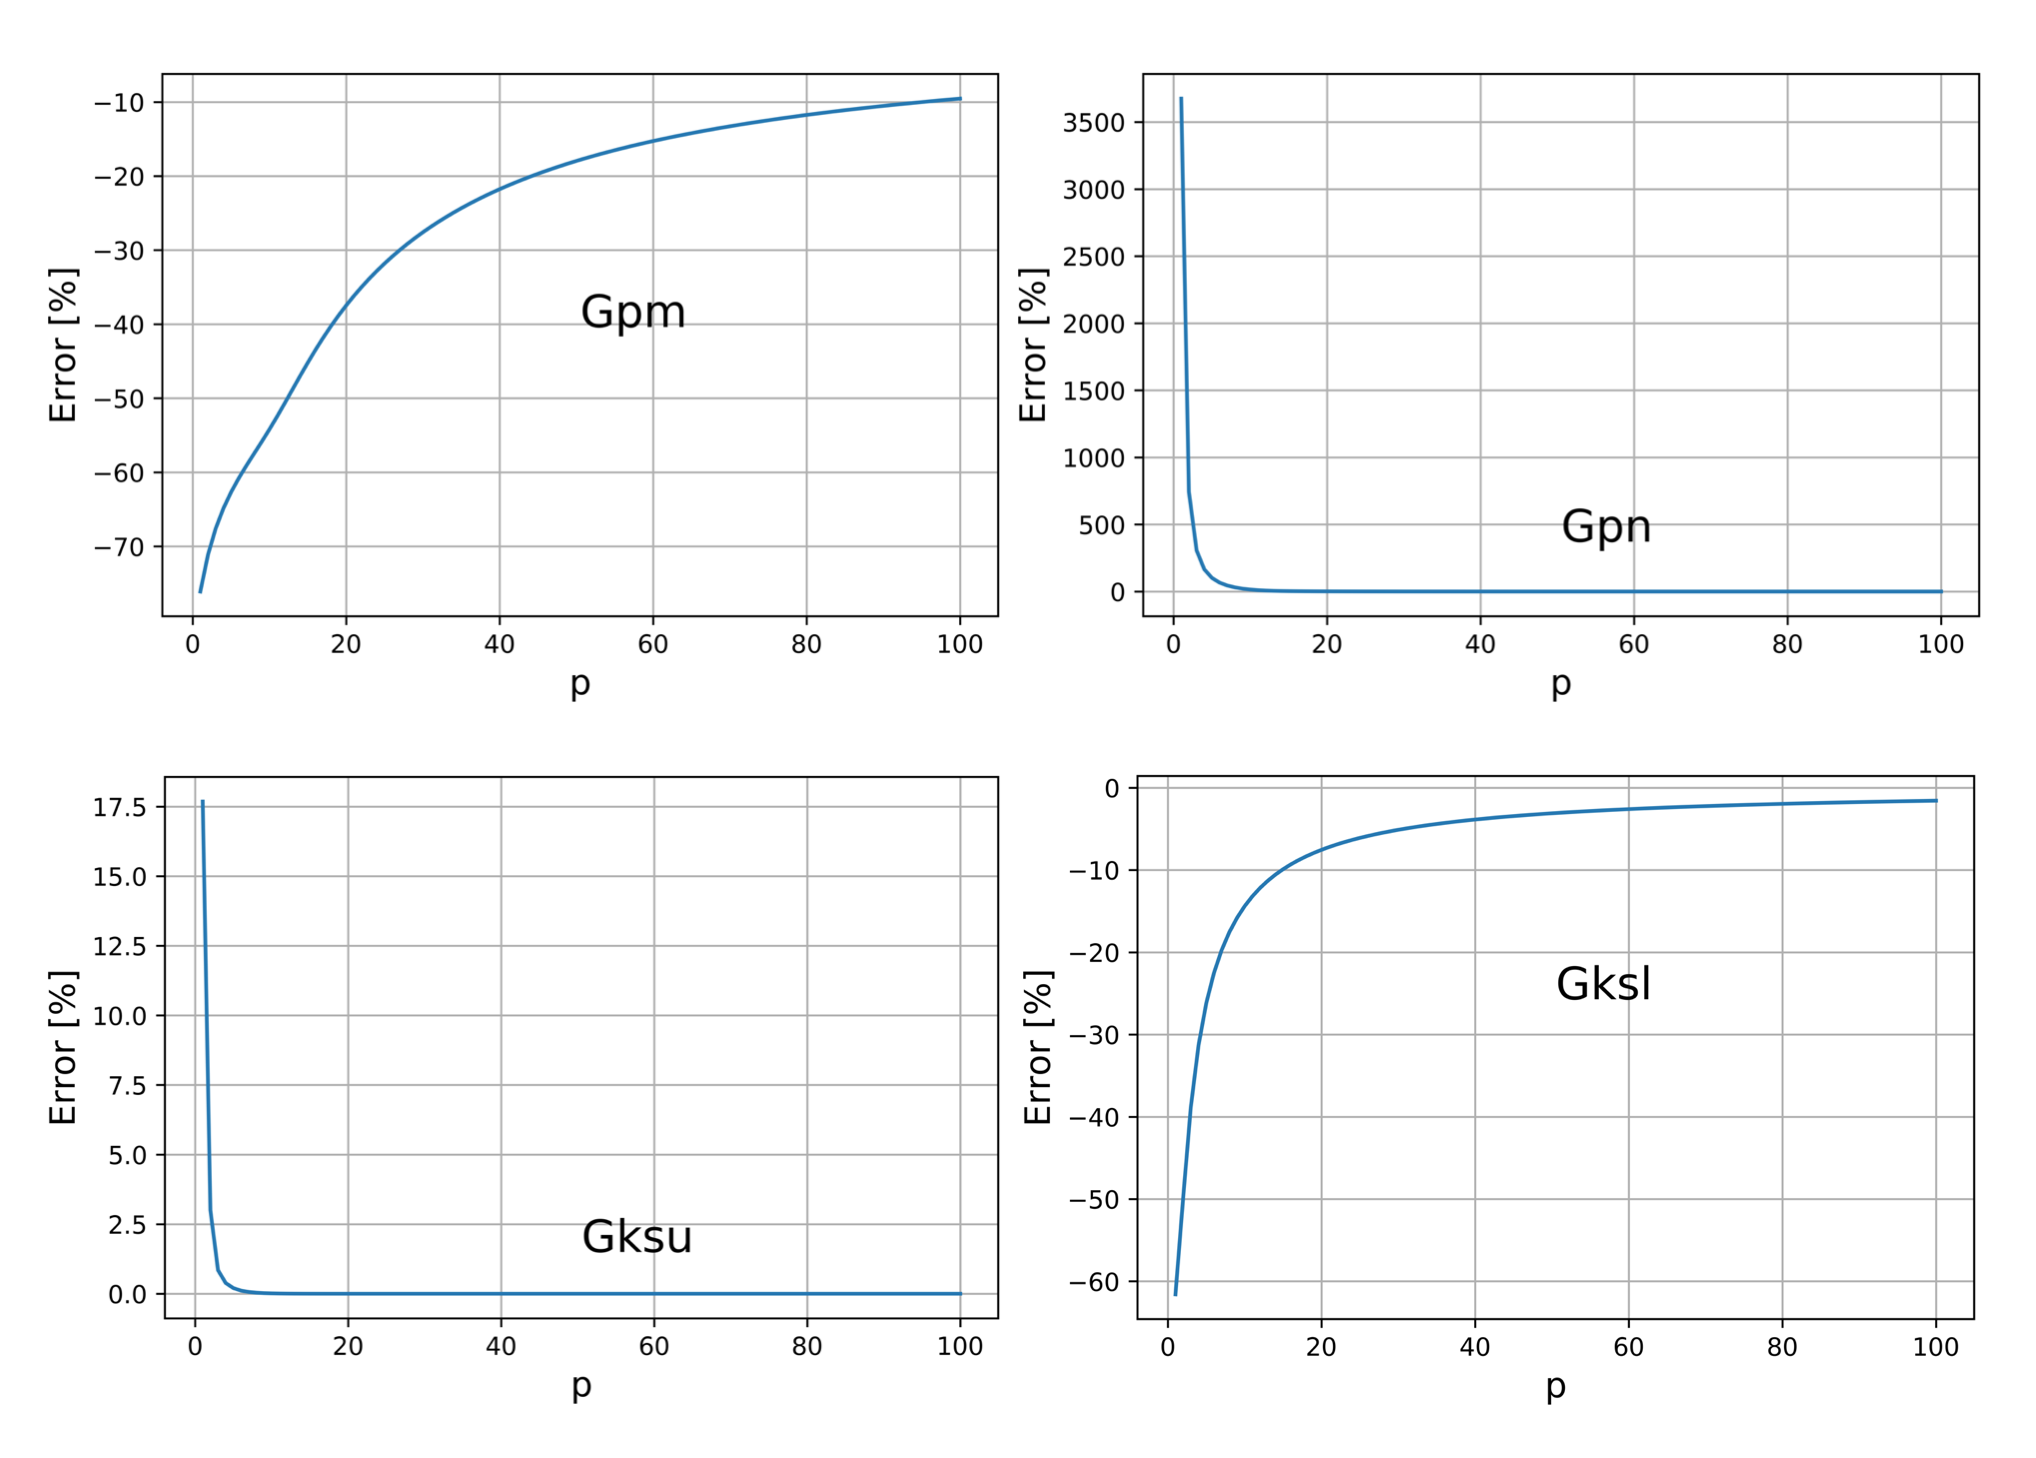
\includegraphics[width = 0.7\textwidth]{./Immagini/3_4.png}
	\caption{Effects of the aggregation parameter $P$ on the relative error}
	\label{fig:3_4}
\end{figure}
From these graphics we can saw the difference between a lower bounded function ($G_{KS}^L$ and $G_{PM}^L$) or an upper bounded function ($G_{KS}^U$ and $G_{PN}^U$), in fact as we can see in the first case the relative error converge to 0 from the bottom, and in the second case from the top. As we can see, as definition, for $p\to\infty$ the relative error go to 0, and that error depends from the aggregation function, the relative error is acceptable for $P\approx 50$ for the upper bounded function, while for the lower bounded the error is still not acceptable. "$P = 50$ is usually a reasonable value that has a maximum relative error of $\approx$ 0.03 for two constraints, and is often used"\cite{stu}.\\
In Fig. \ref{fig:3_5} it's showed an zoom-out to see also the upper-bounded function reach the convergence.
\begin{figure}[H]
	\centering
	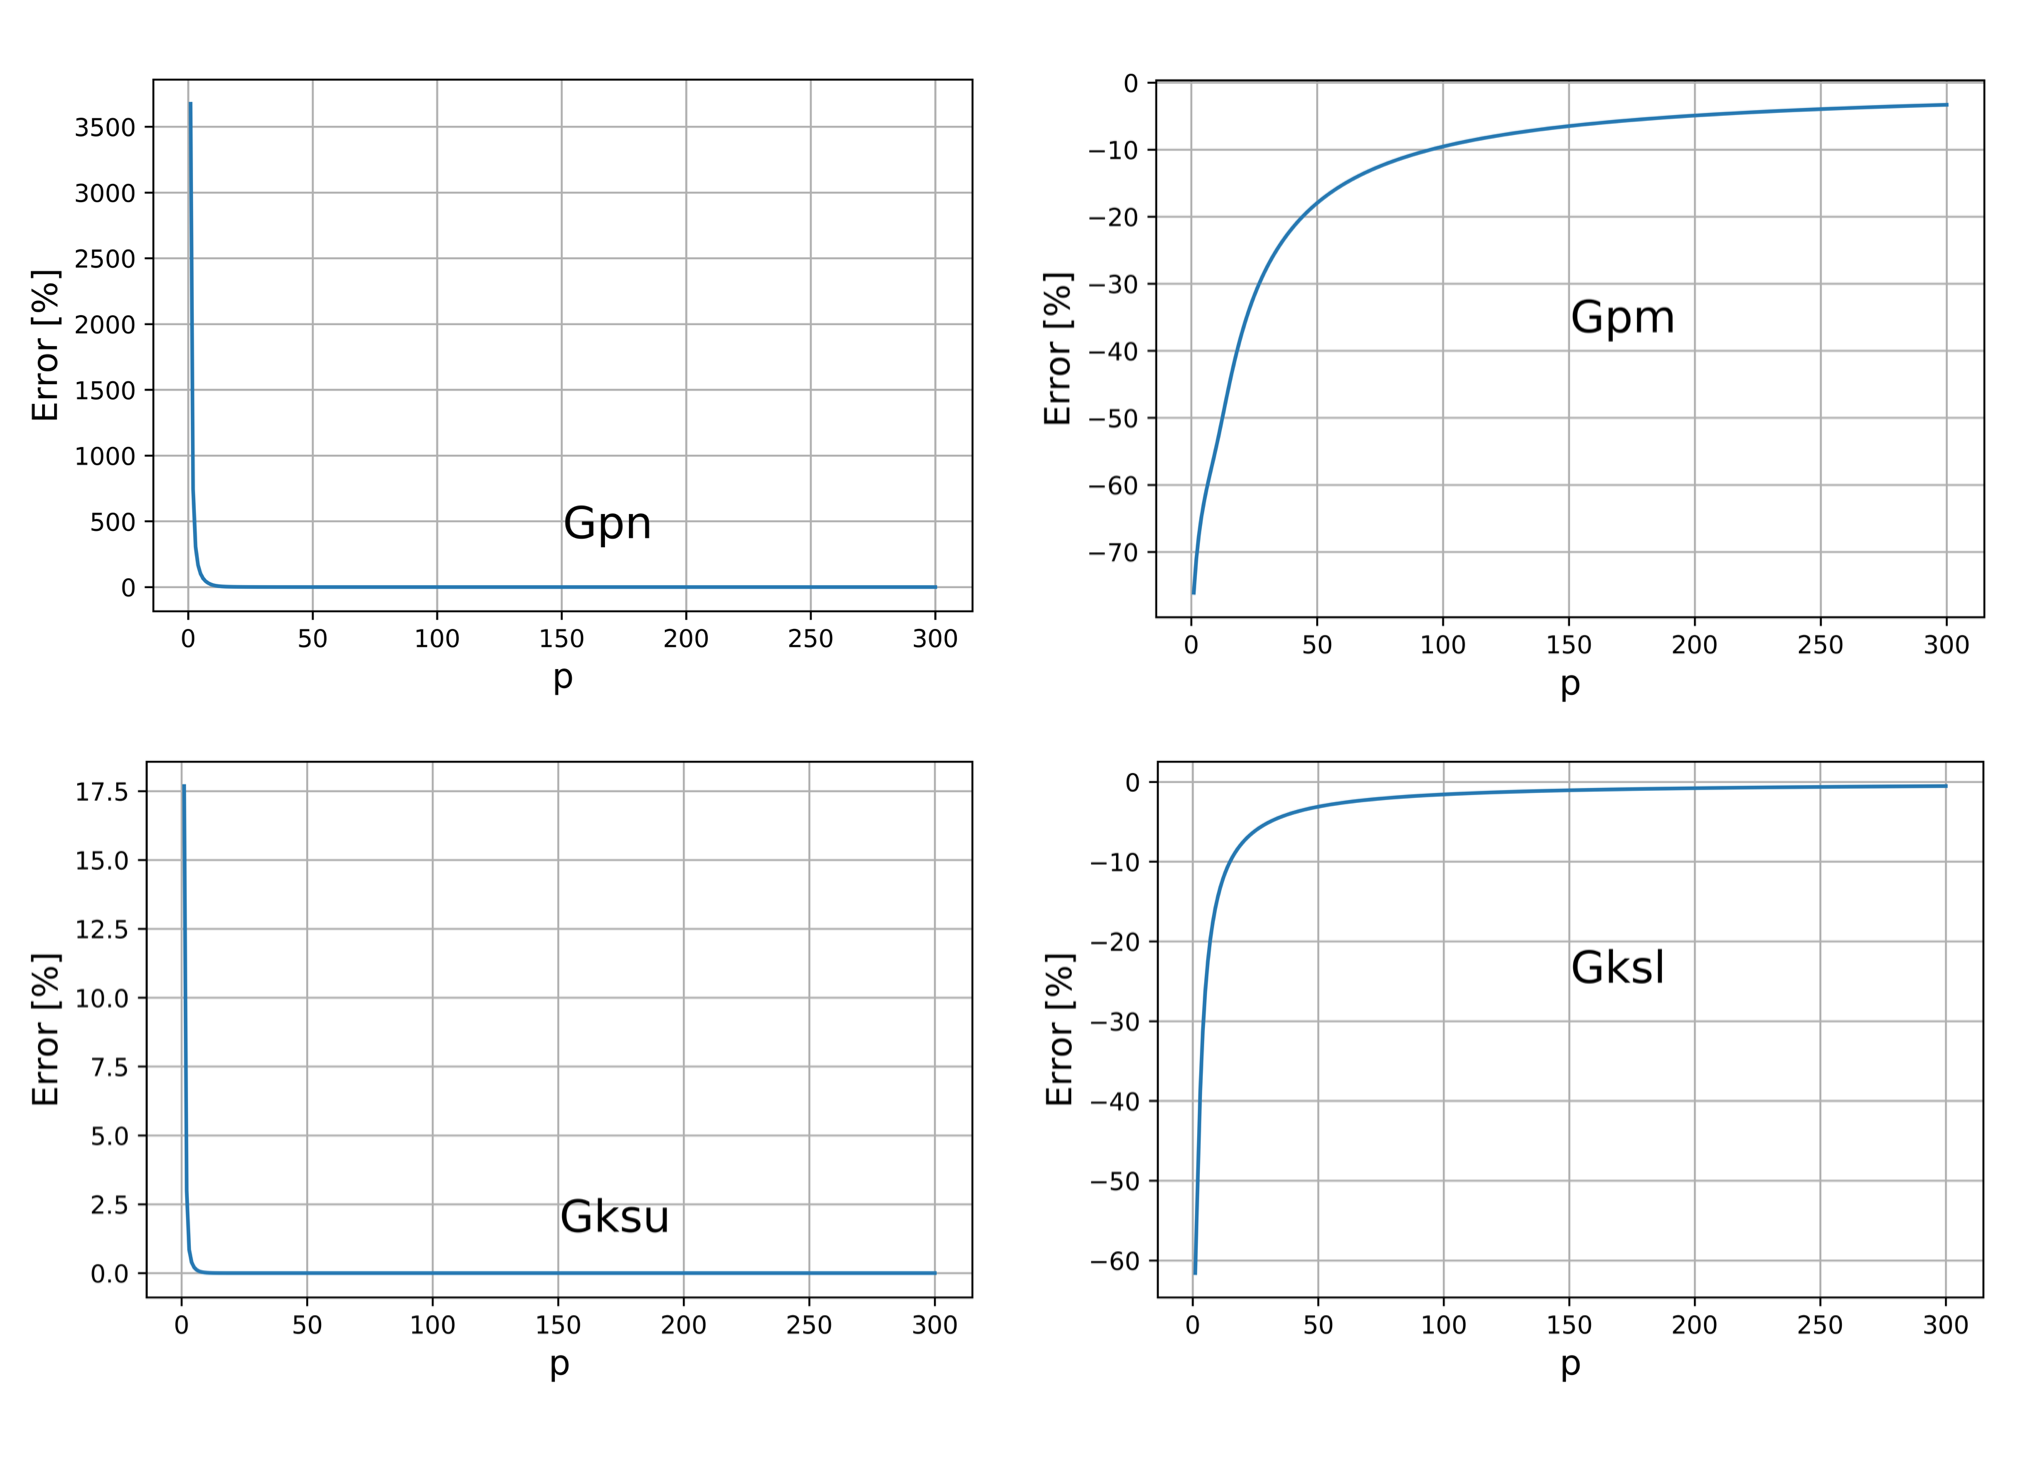
\includegraphics[width = 0.7\textwidth]{./Immagini/3_5.png}
	\caption{Zoom-out of effects of the aggregation parameter $P$ on the relative error}
	\label{fig:3_5}
\end{figure}
\section{Aggregation Component}
To implement the constraint aggregation in the optimization code needs a component that take as input the Von Mises stresses vector and give as output the value of the aggregation function. To be implemented in our script the component should be written in the openMDAO structure. In Fig. \ref{fig:3_6} is represented the flow chart of the component.
\begin{figure}[H]
	\centering
	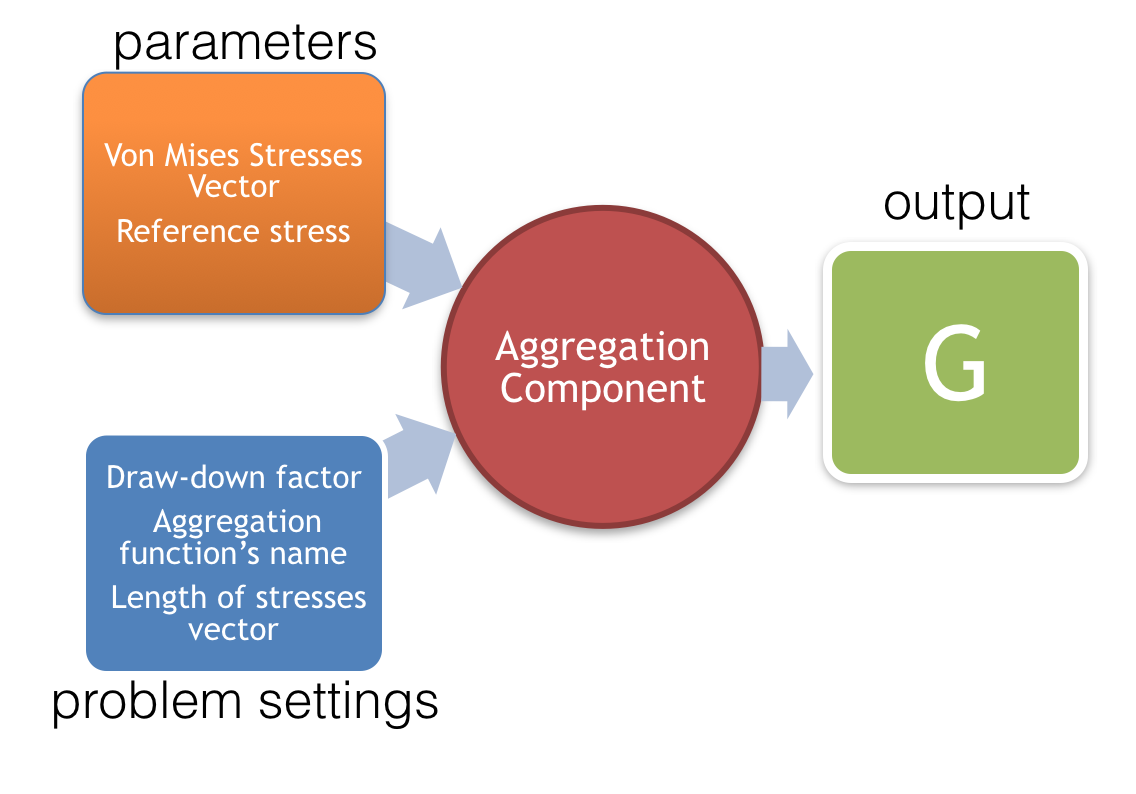
\includegraphics[width = 0.8\textwidth]{./Immagini/3_6.png}
	\caption{Flow chart of the aggregation component}
	\label{fig:3_6}
\end{figure}
The aggregation component takes as input parameters the Von Mises stresses vector $\mathbf{\sigma_{VM}}$ and the reference stress $\sigma_0$ used for the nondimensionalization, connected to the relative variables of the main code between the command \textit{promotes=[*]}; the settings of the aggregation are declared in the main script and are input for the component, there are the value choose for the draw-down factor, the aggregation function selected and the dimension of the vector. Than the component compute the aggregation function and give as output it's value, joined to the constraints functions to be used during the optimization process.\\
In Fig. \ref{fig:3_7} it's showed how the component is made, in the openMDAO structure and the links between the variables:
\begin{figure}[H]
	\centering
	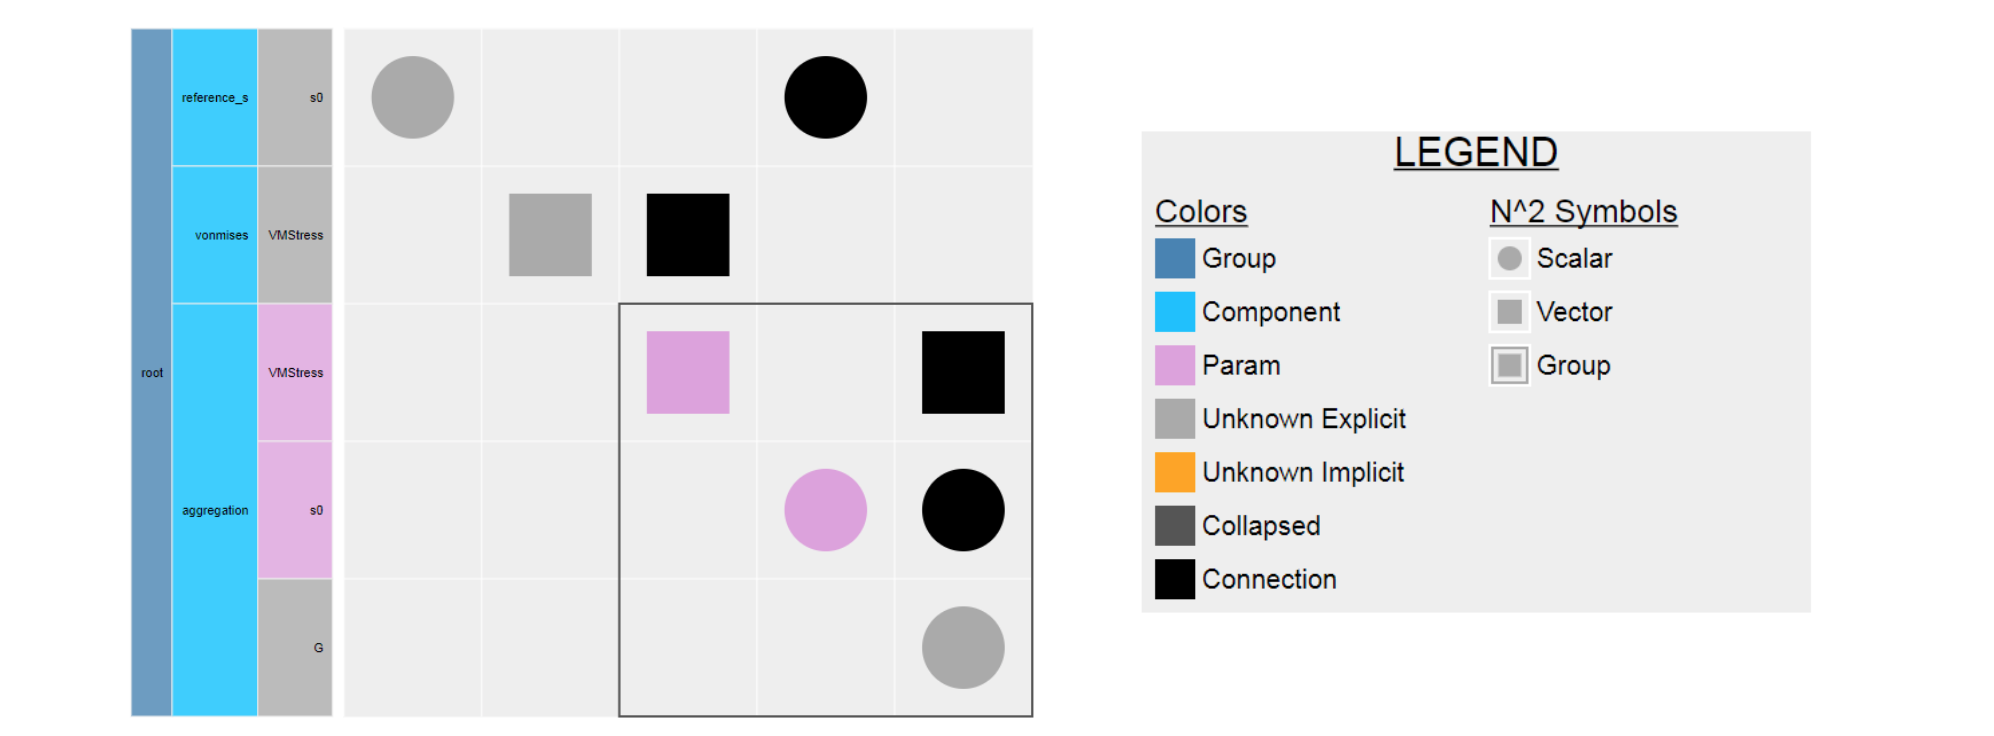
\includegraphics[width = 1\textwidth]{./Immagini/3_7.png}
	\caption{openMDAO structure of the aggregation component}
	\label{fig:3_7}
\end{figure}

%
\chapter{Reduced Model for MDA Loop} 
\label{chapter4}
\section{Introduction to the Reduced Model}
The aerolastic analysis is one of the costly operation in the optimization process, in fact many computation must be performed, with different software; to perform an aerolastic analysis a static structural analysis, an aerodynamic analysis and a dynamic structural analysis, for each iteration is required. So to contain the cost of the analysis models with a low computational cost are needed. In parallel with the multidisciplinary design optimization process, Josè Serralta and Dimitrios Glenis, work to the project which the objective is to perform a model reduction from a complex 3D geometry to a simpler one with a computational cost compatible with the one required for the optimization process and yet a sufficient accuracy for a satisfactory preliminary design, as is illustrated in their report \cite{bru}. A modal analysis will be performed on both the complete and the reduced model, to check that their dynamic are indeed similar. Then, the reduced model will be used for the static, dynamic and aeroelastic analysis in the optimization loop.\\
In the preliminary design phase simplified beams models, knowns as stick models, are used to perform static and dynamic aeroelastic analysis, to have some preliminary results without high cost. During the last stages of the design, high fidelity detailed 3D FEM models are used for design validation and optimization, but this kind of models are too expensive for the MDO process. Thus, condensed models are created for dynamic simulations, using reduction techniques to develop models which are sufficiently simple but sophisticated enough to predict the dynamic behavior \cite{bomb}. Guyan reduction technique was one of the first to appear, it is one of the most popular condensation methods and it is included in many commercial FEM codes \cite{ter}.
\subsection{Approach for the Reduced Model}
In Fig. \ref{fig:4_1} are showed the different modeling levels for a wing. As we can see the structure of the wing can be represented with a box-like model, where the semi-monocoque structure, composed by discrete stiffeners, like stringer, and thin walled panels, like the cover skin and ribs, is modeled and meshed using FEM elements, like beam and shell elements. Another approach to model the wing is using a beam-like model, where each beam element represent the stiffness properties of an associated wing strip. \\
In literature two approaches are considered:
\begin{itemize}
	\item Reduction techniques, such as guyan or IRS \cite{don}, can be used to reduce the original 3D FEM model with $N$ degree of freedom to one which a much smaller number of nodal points $M < < N$. The DoF of the reduced model are referred as masters, and the deleted ones as slaves. The selection of the master nodes is very important, although there exist iterative methods which make their selection much less critical \cite{qui}. The result of condensation is still a 3D model, but with less nodes.
	\item Generating a stick model by extracting the stiffness properties of the full 3D FEM model and applying them to a set of beam elements extending along the structure’s elastic axis \cite{ite}. In this case the full model is not reduced, but a new equivalent FEM model is built.
\end{itemize}
The reduction techniques are usually used for dynamic analysis, while for the aeroelastic studies the condensation to stick models is more used, so for this project the second approach is adopted.\\
So the main idea for the reduced model is to start from the detailed FEM model with the shell elements, perform an static analysis with exploration load, and from that analysis compute the stiffness and inertial properties of a section, then for each section one beam elements are associated to one section, and we set its stiffness and inertial properties the properties of the respective section.\\

\begin{figure}[H]
	\centering
	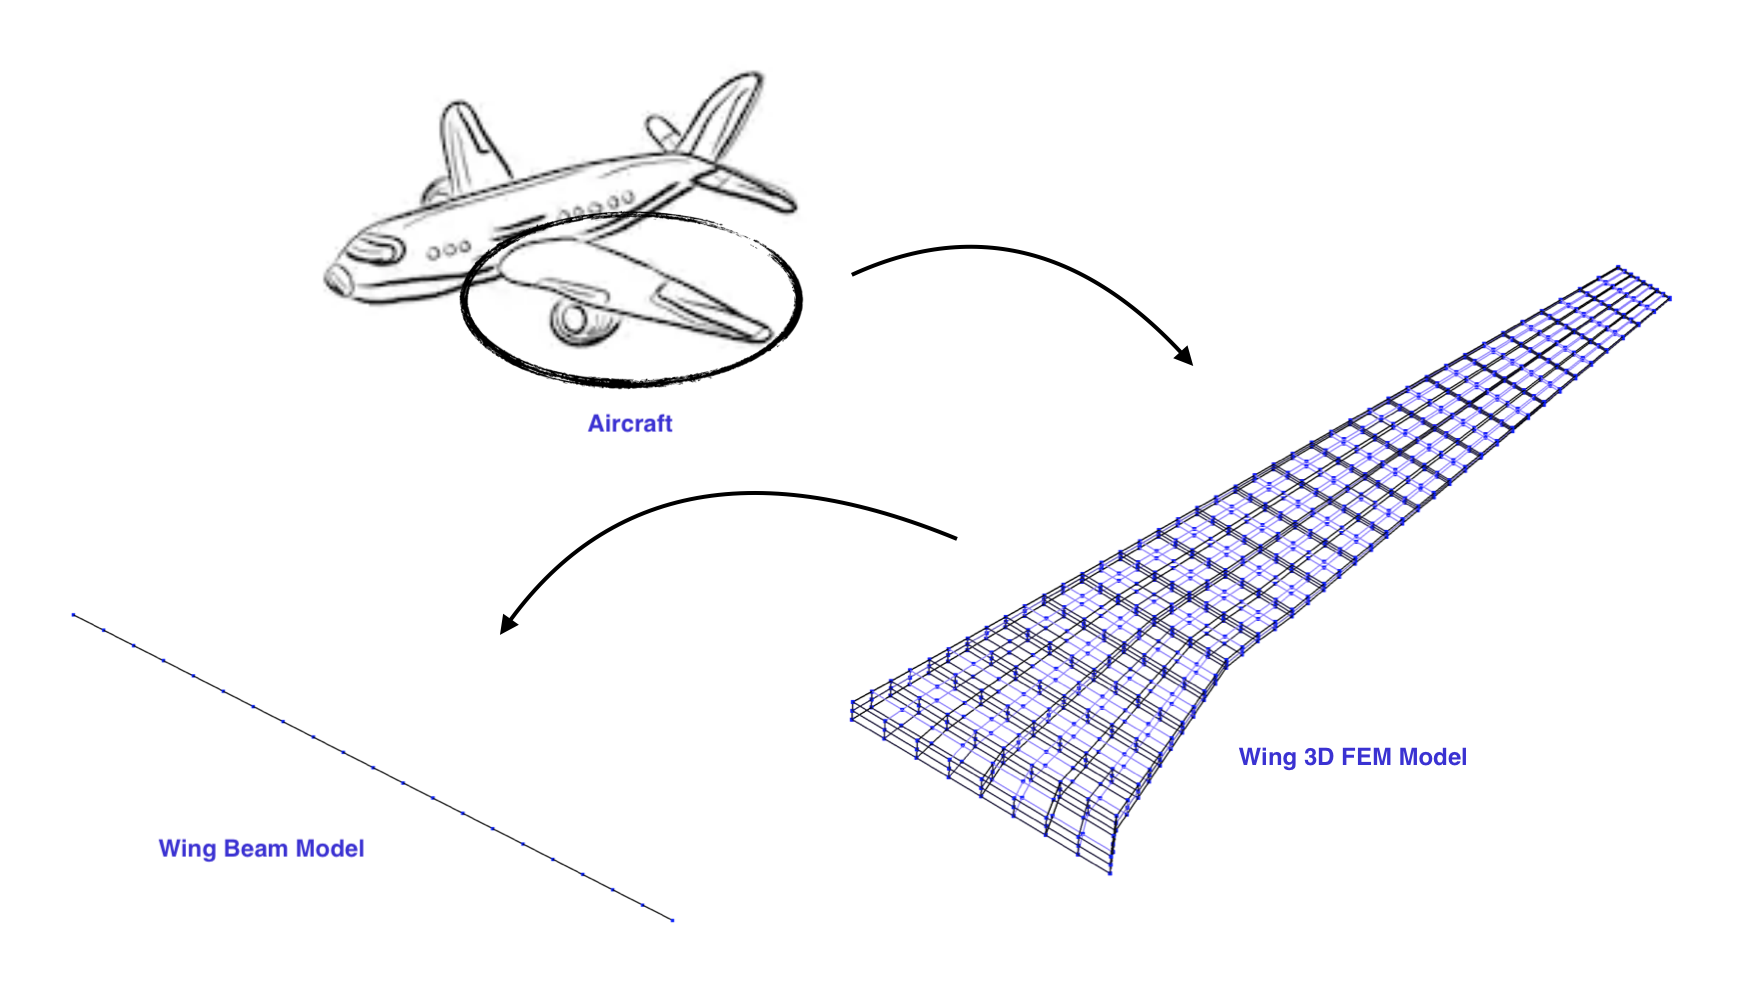
\includegraphics[width = 0.8\textwidth]{./Immagini/4_1.png}
	\caption{Different modeling levels }
	\label{fig:4_1}
\end{figure}
\section{Structure of the Code}
In this part we will see how the stick model is obtained from the full model, and how the validation of the stick model is performed. In Fig. \ref{fig:4_2} is represented the flow chart of the reduction model:
\begin{figure}[H]
	\centering
	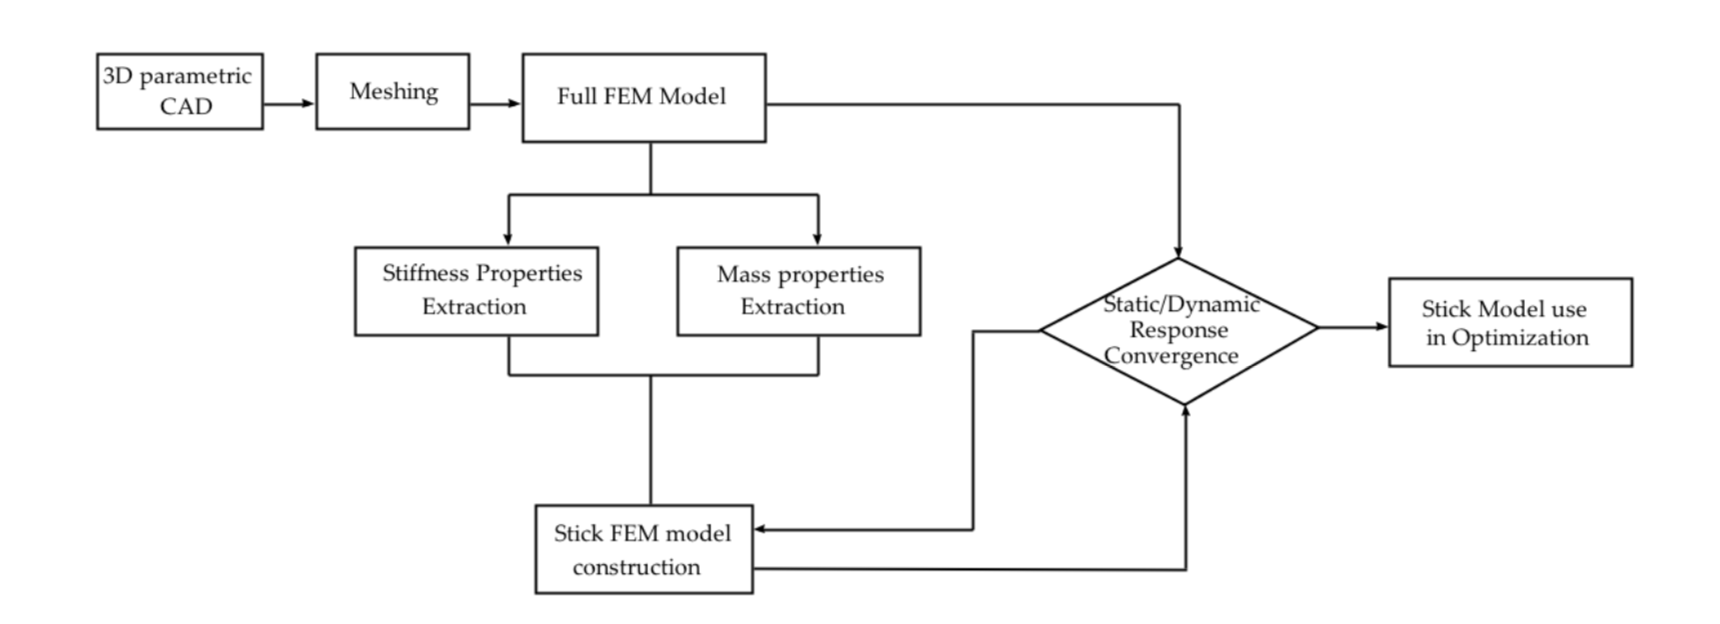
\includegraphics[width = 1\textwidth]{./Immagini/4_2.png}
	\caption{Flow chart of the reduced model code }
	\label{fig:4_2}
\end{figure}
The Full FEM model is created using the geometry component, that we discuss in the chapter 2. From the full FEM model the mass and stiffness properties of the section, which we split our model, are extracted using the Nastran Weight Generator instrument. Then the stick model be created, importing the mass and stiffness properties of each section in one beam element. The stick model need now to be validated, one static analysis and one modal analysis will be performed on the stick model, then the result will be compared to the result of the same analysis performed on the full model. While the results is not acceptable some corrective coefficient will be changed until the convergence of the relative error is guaranteed. When the stick model is validated, it can be used in the optimization code, in particular in the MDA loop, to obtain a gain on the computational cost of this operation.
\subsection{Creation of the FEM model}
To create the FEM model of the stick model the procedure it's the same of the creation of the FEM model of the full model. As we saw in the chapter 2, after the geometry component creates the \textit{.igs} file, and after the program gmsh create the FEM mesh, the structure component write the bfd file, putting the properties of each elements in a NASTRAN card, from a template \textit{.bdf} file. In this case we use another \textit{.bdf} template, where there are just BAR elements (the beam elements in the NASTRAN95 language). For this part just the number of the elements, equal to the number of the section used to split the full model, and the position of the nodes are required. For each element also a lumped mass will be created, and for the moment it's value is 0 and it's located in the first node of the element, when we will have the information about the mass propierties, using the offset command we will change the effective position of the lumped mass. At the end of this process we will have a \textit{.bdf file} of a stick model, that present $N$ BAR elements and $N$ lumped mass, but without information about the material and inertia properties. In Fig. \ref{fig:4_3} are schematized what this component do:
\begin{figure}[H]
	\centering
	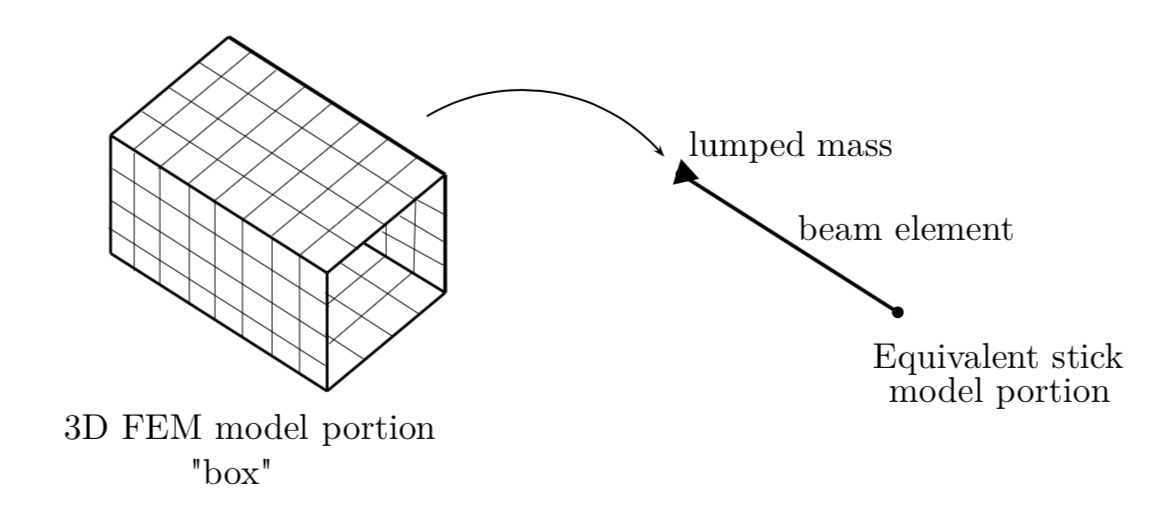
\includegraphics[width = 0.8\textwidth]{./Immagini/4_3.png}
	\caption{Schematization of the creation of the stick model }
	\label{fig:4_3}
\end{figure}
\subsection{Extraction of Stiffness and Inertia Properties}
Starting from the 3D FEM model of the structure, we split it into section called boxes, which could be delimited by the ribs of the wing. The object is to build a 1D model in which each box is represented from an equivalent beam element. To do this as first we need to determinate the stiffness properties ($A,I_y,I_z,J$) and the inertia properties ($m,x_G,I_G$) to give to the beam element so it's representative of the box. 
\subsubsection{Stiffness Properties}
The flexibility matrix \textbf{C} of each box is obtained from the displacements due to a set of unitary loads applied to one of its sections. \cite{bru}.
\begin{figure}[H]
	\centering
	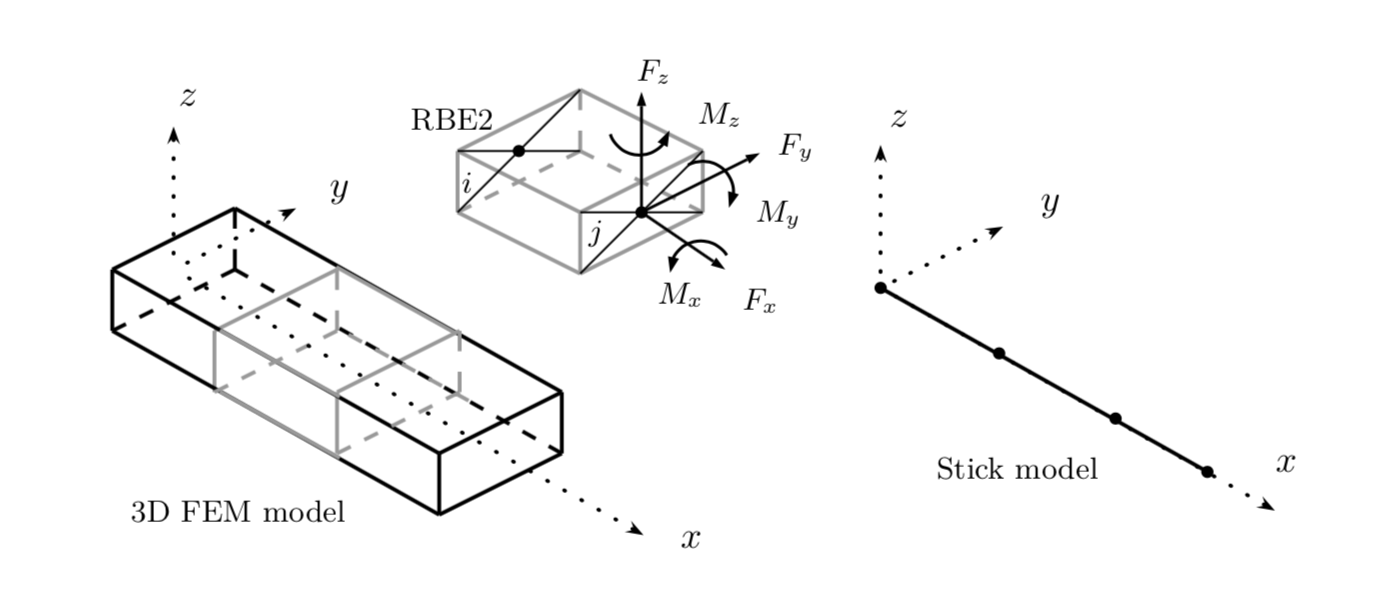
\includegraphics[width = 0.8\textwidth]{./Immagini/4_4.png}
	\caption{Detailed model subdivisions and unitary loads for the extraction}
	\label{fig:4_4}
\end{figure}
In Fig.\ref{fig:4_4} is showed a box with the 2 associated nodes of the reduced model (nodes \textit{i} and \textit{j}). To compute the flexibility matrix \textbf{C} a set of six unitary loads are applied at node \textit{j} and the consequent displacements are measured at nodes \textit{i} and \textit{j}. \\
Let $\mathbf{C_i}$ and $\mathbf{C_j}$ be the flexibility matrices relating loads at \textit{j} with displacements at \textit{i} and \textit{j} respectively. If a unitary load vector \textbf{F} is applied, then from $C\dot F = U$ the associated displacements \textit{u} provides a column of matrix \textbf{C}. In this way, with the displacements from the six unitary loads, the six columns of matrices $\mathbf{C_i}$ and $\mathbf{C_j}$ are built. \cite{bru}\\
The $\mathbf{C_i}$ and $\mathbf{C_j}$ are the flexibility matrices relating loads at node \textit{j} with displacement at nodes \textit{i} and \textit{j} respectively. We can obtain the flexibility matrix of the box from the forces and strains. Strains are approximated obtained from these relations:
\begin{equation*}
\epsilon_x=\frac{u_{x_j}-u_{x_i}}{\Delta x}; \qquad \gamma_y=\frac{u_{y_j}-u_{y_i}}{\Delta x}; \qquad \gamma_z=\frac{u_{z_j}-u_{z_i}}{\Delta x}
\end{equation*}
\begin{equation*}
\kappa_x=\frac{\theta_{x_j}-\theta_{x_i}}{\Delta x}; \qquad \gamma_y=\frac{\theta_{y_j}-\theta_{y_i}}{\Delta x}; \qquad \gamma_z=\frac{\theta_{z_j}-\theta_{z_i}}{\Delta x}
\end{equation*}
where $u_{x_j}$ is the displacement in \textit{x}-direction at node \textit{j}, $\theta_{x_j}$ is the rotation in \textit{x}-direction at node \textit{j}, and the same for the others, $\Delta x$ is the length of the box. So the flexibility matrix of the box will be:
\begin{equation*}
\mathbf{C}=\frac{\mathbf{C_j}-\mathbf{C_i}}{\Delta x}
\end{equation*}
from that we can obtain the stiffness matrix of the box from:
\begin{equation*}
\mathbf{K}=\mathbf{C^{-1}}
\end{equation*}
From the stiffness matric we can obtain the section proprieties, from the following relation:
\begin{equation*}
\begin{pmatrix}
F_x\\
F_y\\
F_z\\
M_x\\
M_y\\
M_z\\
\end{pmatrix} =
\begin{bmatrix}
A_{11}&0&0&0&A_{12}&A_{13}\\
0&S_{11}&S_{12}& S_{13}&0&0   \\
0&S_{21}&S_{22}& S_{23}&0&0   \\
0&S_{31}&S_{32}& S_{33}&0&0   \\
A_{21}&0&0&0&A_{22}&A_{23}\\
A_{31}&0&0&0&A_{32}&A_{33}\\
\end{bmatrix}
\begin{pmatrix}
\epsilon_x \\
\gamma_y \\
\gamma_z \\
\kappa_x \\
\kappa_y \\
\kappa_z 
\end{pmatrix}
\end{equation*}
Where $A_{ij}$ and $S_{ij}$ are the stiffness terms associated to axial and shear sets. So from the constitutive equation it's possible to determinate the section properties:
\begin{equation*}
\mathbf{A} =
\begin{bmatrix}
A_{11}&0&0\\
&A_{22}&0\\
sym&&A_{33}
\end{bmatrix}=
\begin{bmatrix}
EA&0&0\\
&EI_y&0\\
sym&&EI_z
\end{bmatrix}
\end{equation*}
\begin{equation*}
\mathbf{S} =
\begin{bmatrix}
S_{11}&0&0\\
&S_{22}&0\\
sym&&S_{33}
\end{bmatrix}=
\begin{bmatrix}
GA_y&0&0\\
&GA_z&0\\
sym&&GJ
\end{bmatrix}
\end{equation*}
From this it's possible to extract the section properties $A,I_y,I_z,J$ to give to the beam element to be representative of the box section.
\subsubsection{Inertia Properties}
The inertia properties of each box are extracted using the \textit{NASTRAN grid point weight generator} \cite{msc}, which generate an output file containing the information relative to the position of the center of gravity $X_G$, the mass $m$ and inertias $I$ of the box. In Fig. \ref{fig:4_5} is showed an example of the output file. From this information we will change the position and the properties of the lumped mass that we create in the first phase. Since the mass of the boxes are represented from the lumped mass, the density of the material is set to 0.
\begin{figure}[H]
	\centering
	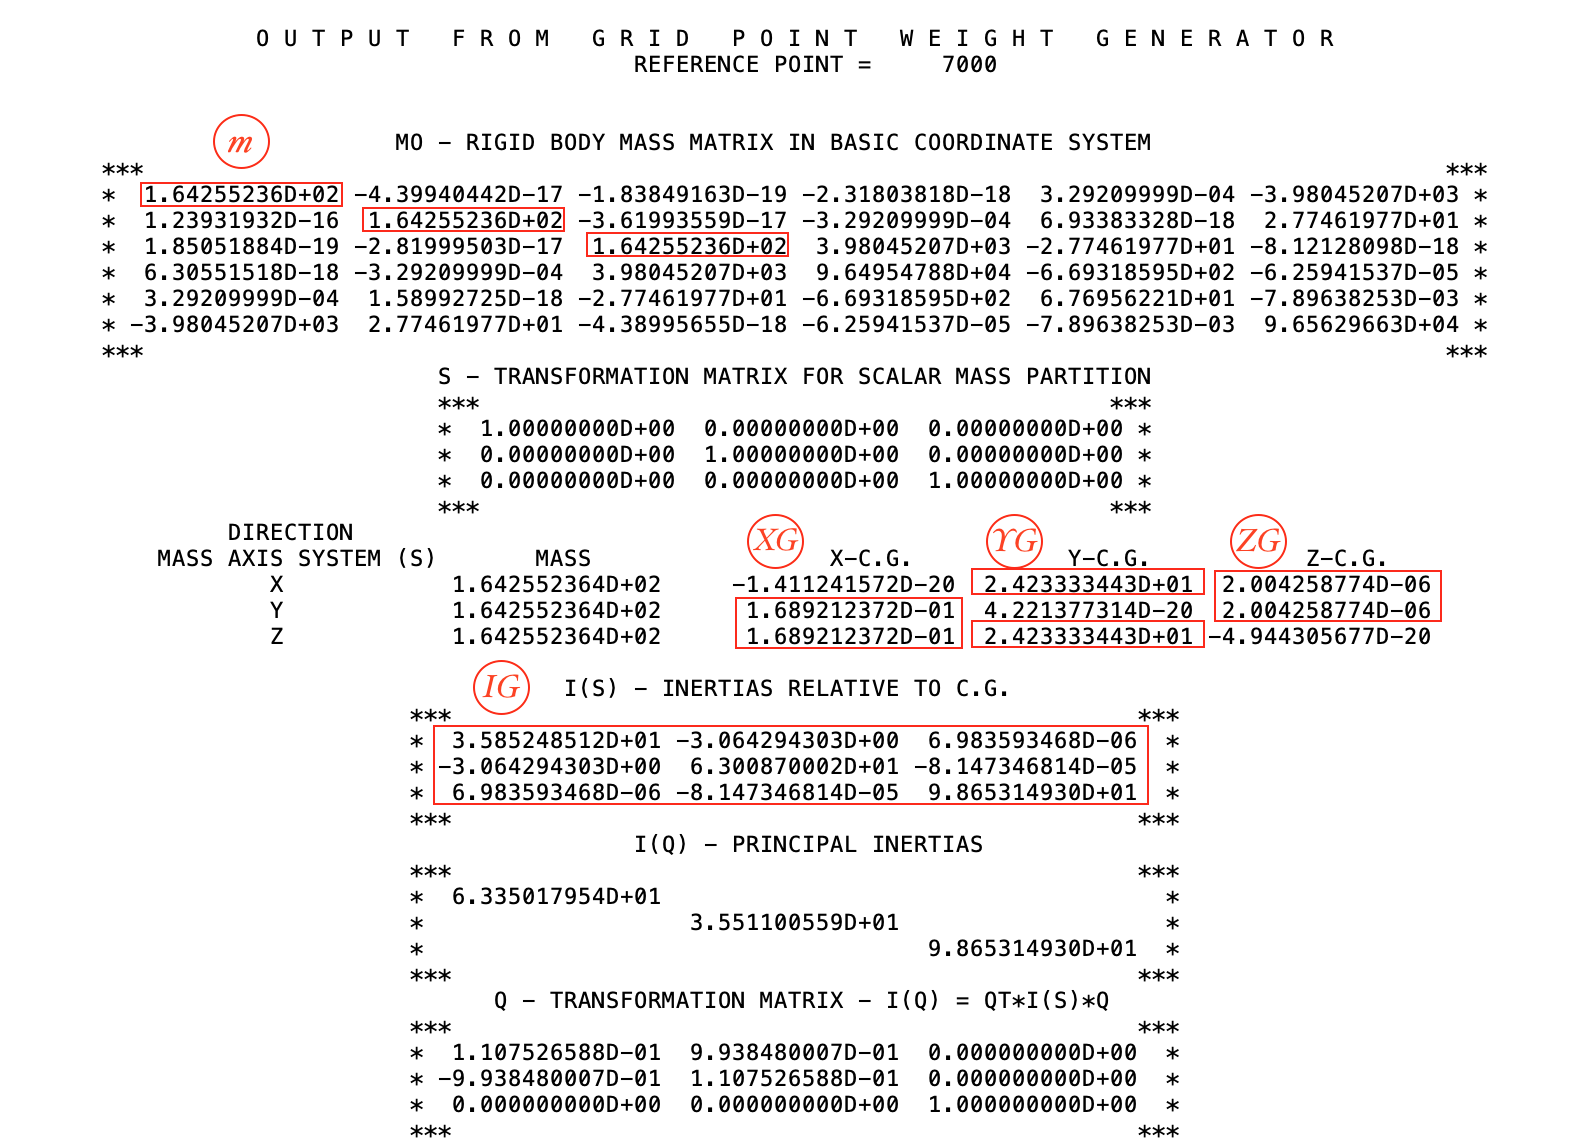
\includegraphics[width = 1\textwidth]{./Immagini/4_5.png}
	\caption{NASTRAN grid point weight generator output file}
	\label{fig:4_5}
\end{figure}
At the end of the process the beam element has the stiffness and inertia properties of the box, as the Fig. \ref{fig:4_6} shows:
\begin{figure}[H]
	\centering
	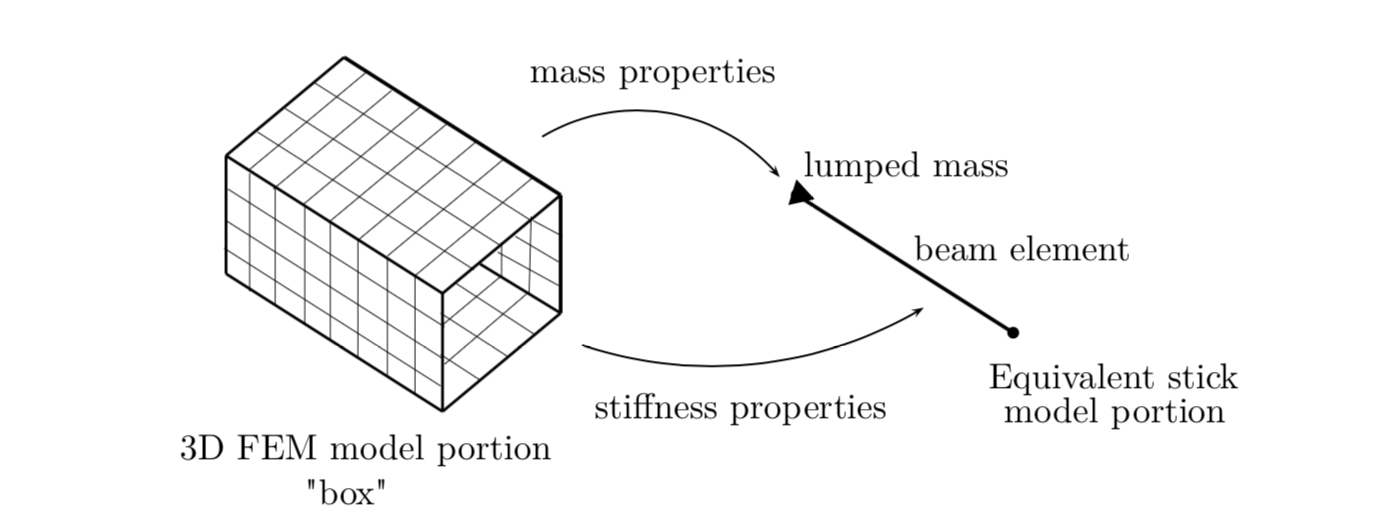
\includegraphics[width = 1\textwidth]{./Immagini/4_6.png}
	\caption{Schematization of the creation of the stick model and importing of the properties}
	\label{fig:4_6}
\end{figure}
\section{Validation of the Stick Model}
For the validation of the stick model two comparison have been done, one on the static response results, in terms of displacement and rotation of the nodes, and one on the modal analysis, in terms of natural frequencies and modal shapes. In both the cases to allow the comparison, since the number of nodes and their position is different, a series of nodes have been added in the full model, in particular we add in the full model the same nodes used for the stick model in the same relative position, then we connected these nodes to the structural nodes of the full model between rigid connection. In that way we can comparison the displacement, the eigenvector and the eigenvalue of the two different models.
\subsection{Comparison of the Static Response}
To do the comparison of the static response an exploration load have been applied at the wing tip. To determinate the displacements and the rotation in all the direction 6 different load have been applied, 3 force of 1 $N$ applied on the $x, y$ and $z$ direction, $F_x,F_y$ and $F_z$, and 3 moments of 1 $N\ mm$, $;M_x,M_y$ and $M_z$.\\
In the Fig. \ref{fig:4_7} there are the results obtained from the comparison.\\
As we can see the errors on the displacements are $\approx 15\%$ at the wingtip, while the errors on the rotation are smaller, $\approx 10\%$, and $\approx 1\%$ on the horizontal rotation $\theta_y$. \\
\begin{figure}[H]
	\centering
	\subfigure[Longitudinal displacement $u_x$]{
			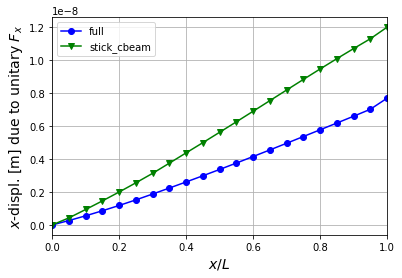
\includegraphics[width = 0.4\textwidth]{./Immagini/4_7.png}
		\label{fig:subfig1}
	}
	\subfigure[Torsional rotation $\theta_x$]{
		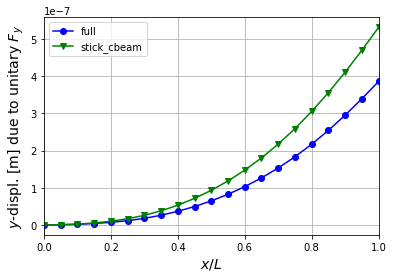
\includegraphics[width = 0.4\textwidth]{./Immagini/4_8.png}
		\label{fig:subfig2}
	}
	\subfigure[Horizontal displacement $u_y$]{
	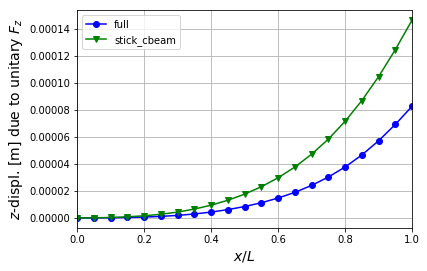
\includegraphics[width = 0.4\textwidth]{./Immagini/4_9.png}
	\label{fig:subfig1}
}
\subfigure[Horizontal rotation $\theta_y$]{
	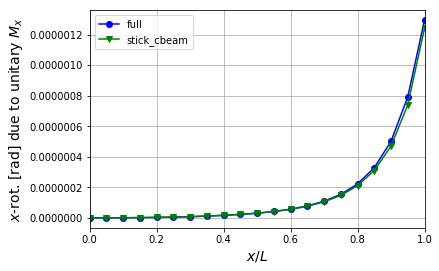
\includegraphics[width = 0.4\textwidth]{./Immagini/4_10.png}
	\label{fig:subfig2}
}
	\subfigure[Vertical displacement $u_z$]{
	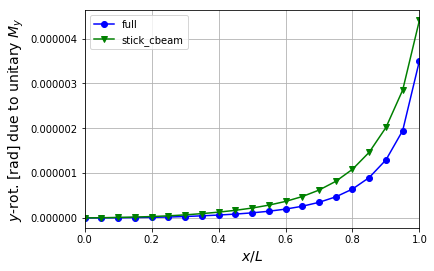
\includegraphics[width = 0.4\textwidth]{./Immagini/4_11.png}
	\label{fig:subfig1}
}
\subfigure[Vertical rotation $\theta_z$]{
	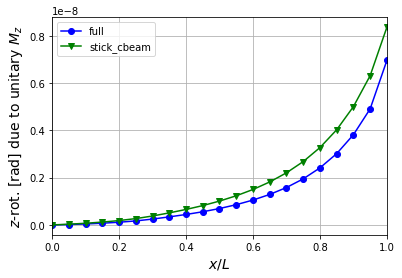
\includegraphics[width = 0.4\textwidth]{./Immagini/4_12.png}
	\label{fig:subfig2}
}
\caption[Optional caption for list of figures]{Comparison of the static response }
	\label{fig:4_7}
\end{figure}

To get better results it's possible to adopt a correction on the Young module $E$ and on the shear module $G$, using virtual modules obtained from the relative error on the displacements and rotation:
\begin{equation*}
E_{corr}=\frac{u_{z|stick}}{u_{z|full}}E;\qquad G_{corr}=\frac{\theta_{x|stick}}{\theta_{x|full}}G
\end{equation*}
\subsection{Comparison of the Modal Properties}
To do the comparison of the modal properties we compare as first the modal shapes of the two model, and after the natural frequencies. Also in this case the extra nodes are used in the full model to have a compatibility for the two modal shapes. To compare the modal shape the Modal Assurance Criterion \textbf{MAC} have been used.
\subsubsection{Modal Assurance Criterion MAC}
The function of the modal assurance criterion (MAC) is to provide a measure of consistency between estimates of a modal vector. \cite{mac2} The Modal Assurance Criterion is a vector correlation index frequently used in experimental dynamics to quantify the similarity of mode shapes\cite{mac}.\\
This criterion is based on the computation of a normalized scalar product of the eigenvector of the system given by:
\begin{equation*}
MAC(\mathbf{\Phi_1},\mathbf{\Phi_2})=\frac{(\mathbf{\Phi_1^T}\cdot \mathbf{\Phi_2}^T)}{||\mathbf{\Phi_1}||^2\cdot||\mathbf{\Phi_2}||^2} \qquad \qquad 0\le MAC \le 1
\end{equation*}
where $\mathbf{\Phi_1}$ and $\mathbf{\Phi_2}$ are the eigenvector related to the modal shape that we want to compare. A value of 1 means that the modal shapes are identical, while a value of 0 means that the modal shapes are not similar at all. In our case we are interested to check the similarity of the first ten modal shapes, to do this we use the eigenvector output of the modal analysis performed with NASTRAN. For each node 6 DoF are present, so we put the vector related to each singol Dof in a single expanded vector to compare them:
\begin{equation*}
\mathbf{\Phi}=[\mathbf{\Phi_{TX}},\mathbf{\Phi_{TY}},\mathbf{\Phi_{TZ}},\mathbf{\Phi_{RX}},\mathbf{\Phi_{RY}},\mathbf{\Phi_{RZ}}]
\end{equation*}
Then 100 comparison of the modal shapes have been done, and the results can be visualized using a matrix with a colour scale, as is showed in Fig. \ref{fig:4_8}.
\begin{figure}[H]
	\centering
	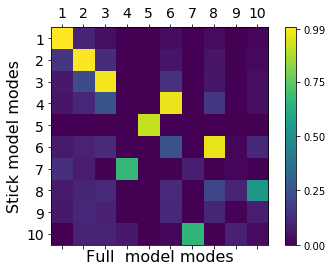
\includegraphics[width = .8\textwidth]{./Immagini/4_13.png}
	\caption{MAC colour matrix for the first ten modal shapes}
	\label{fig:4_8}
\end{figure}
A value of MAC $\approx 1$ means the modal shape of the \textit{i} mode of the full structure $\mathbf{\Phi_i}$  is similar to the modal shape of the \textit{j} mode of the stick structure $\mathbf{\Phi_j}$. \\
As we can see there is a large compatibility on the full bending modes, while the compatability of the torsional and coupled modes is lower.
\subsubsection{Frequencies Comparison}
As we said also a comparison on the first ten natural frequencies have been done. It's important to remark that the frequencies are ordered in ascending order by NASTRAN, so when the error on the frequencies is more than the step from two consecutive frequencies the frequency \textit{i} of the full model cannot be associated at the same mode of the frequency \textit{i} of the stick model. To avoid this problem it's required to order the frequencies using the modal shape order. To order the frequencies a visualization of the modal shapes is required, than we can recognize the type of the mode and associate the correct number to the mode to do the comparison.\\
In Fig. \ref{fig:4_9} there is the bar plot of the error between the full model natural frequencies and the stick model natural frequencies relative to the same modal shape:
\begin{figure}[H]
	\centering
	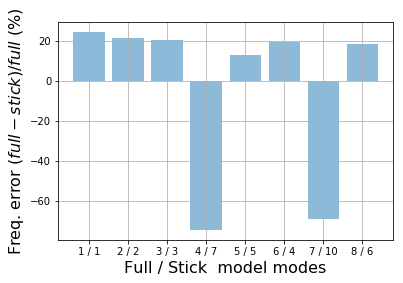
\includegraphics[width = .8\textwidth]{./Immagini/4_14.png}
	\caption{Bar plot of the error between the natural frequencies of the full and stick model}
	\label{fig:4_9}
\end{figure}
In Tab. \ref{tab:t1} there are the value of the first ten frequencies, ordered for the same modal shape for both model, and the relative error computed as:
\begin{equation*}
E= \frac{F_{i_{full}}- F_{i_{stick}}}{F_{i_{full}}}* 100
\end{equation*}
\begin{table}
\begin{tabular}{cccc}
	\toprule
	$Mode $  &  $Full\  model freq. [Hz]$  &  $Stick\  model freq. [Hz]$ & $Relative \ error [\%]$ \\
	\midrule
	$1$  &  $0.73553$  &  $0.55505$ & $ 24.53683 $\\
	$2$  &  $2.46789$  &  $1.92782$ & $ 21.88389 $\\
	$3$  &  $5.4666$  &  $4.33701$  &$  20.66340$\\
	$4$  &  $7.66535$  &  $13.3805$ &$ -74.55837 $  \\
	$5$  &  $9.40136$  &  $8.16675$  &$ 13.13220 $\\
	$6$  &  $9.50287$  &  $7.64263$  &$ 19.57560 $\\
	$7$  &  $13.2508$  &  $22.4217$  &$ -69.21020  $\\
	$8$  &  $14.4031$  &  $11.7250$  &$ 18.5939 $\\
	$9$  &  $19.613$  &  $21.4223$  &$ -9.22500 $\\
	$10$  &  $20.0155$  & $16.4092$ &$ 18.01750 $ \\
	\bottomrule
\end{tabular}
	\caption{Frequencies of full and stick model and relative error}
		\label{tab:t1}
\end{table} 
\section{Modification and Results}
As we can see the validation od the stick model is passed for the static analysis, while for the modal analysis there are some incompatibility. The modal shape related to the torsional and coupled torsional-bending modes are not quite similar, and the results on the natural frequencies present for this mode an error really high, and without sense. A modification at the stick model have been done to avoid this problem. After investigation we understand that the problems are related to the mass distribution, in fact while until the span wing there is a good discretization of the mass of the wing, 20 lumped muss are used, until the cord there isn't a valid distribution, all the lumped mass are positioned until the elastic axis, so the torsional behavior is not correctly represented. A new mass distribution have been implemented to correct this errors.
\subsection{New Mass Distribution}
As we showed in the first section to import the inertia proprieties of the full model on the stick model a series of lumped mass have been used. These lumped mass are positioned in the center of gravity of each box, that's mean that all the mass is concentrated until the elastic axis, then the torsional inertia proprieties of the full model are not imported in the stick model.\\
The idea to avoid this problem is to use a different mass distribution, in particular which takes into account of the distribution of mass until the cord. While just beam elements and lumped mass are used the only way to avoid this problem is to add lumped mass for each section and delocalise that mass from the elastic axis. \\
The new mass distribution provides to create 3 lumped mass for each box, one located in the trailing edge, one located in the center of gravity and one located in the leading edge. The value of the mass is chosen with a linear distribution on the cord, the total mass of the box should be unchanged. To do this the structure component have been modified, as first to compute the value of the 3 lumped mass, then to create the grid point to allocate the mass and finally to modify the \textit{.bdf} file. \\
\newpage
In Fig. \ref{fig:4_10} it's showed how the \textit{.dbf} file is built after the correction:
\begin{figure}[H]
	\centering
	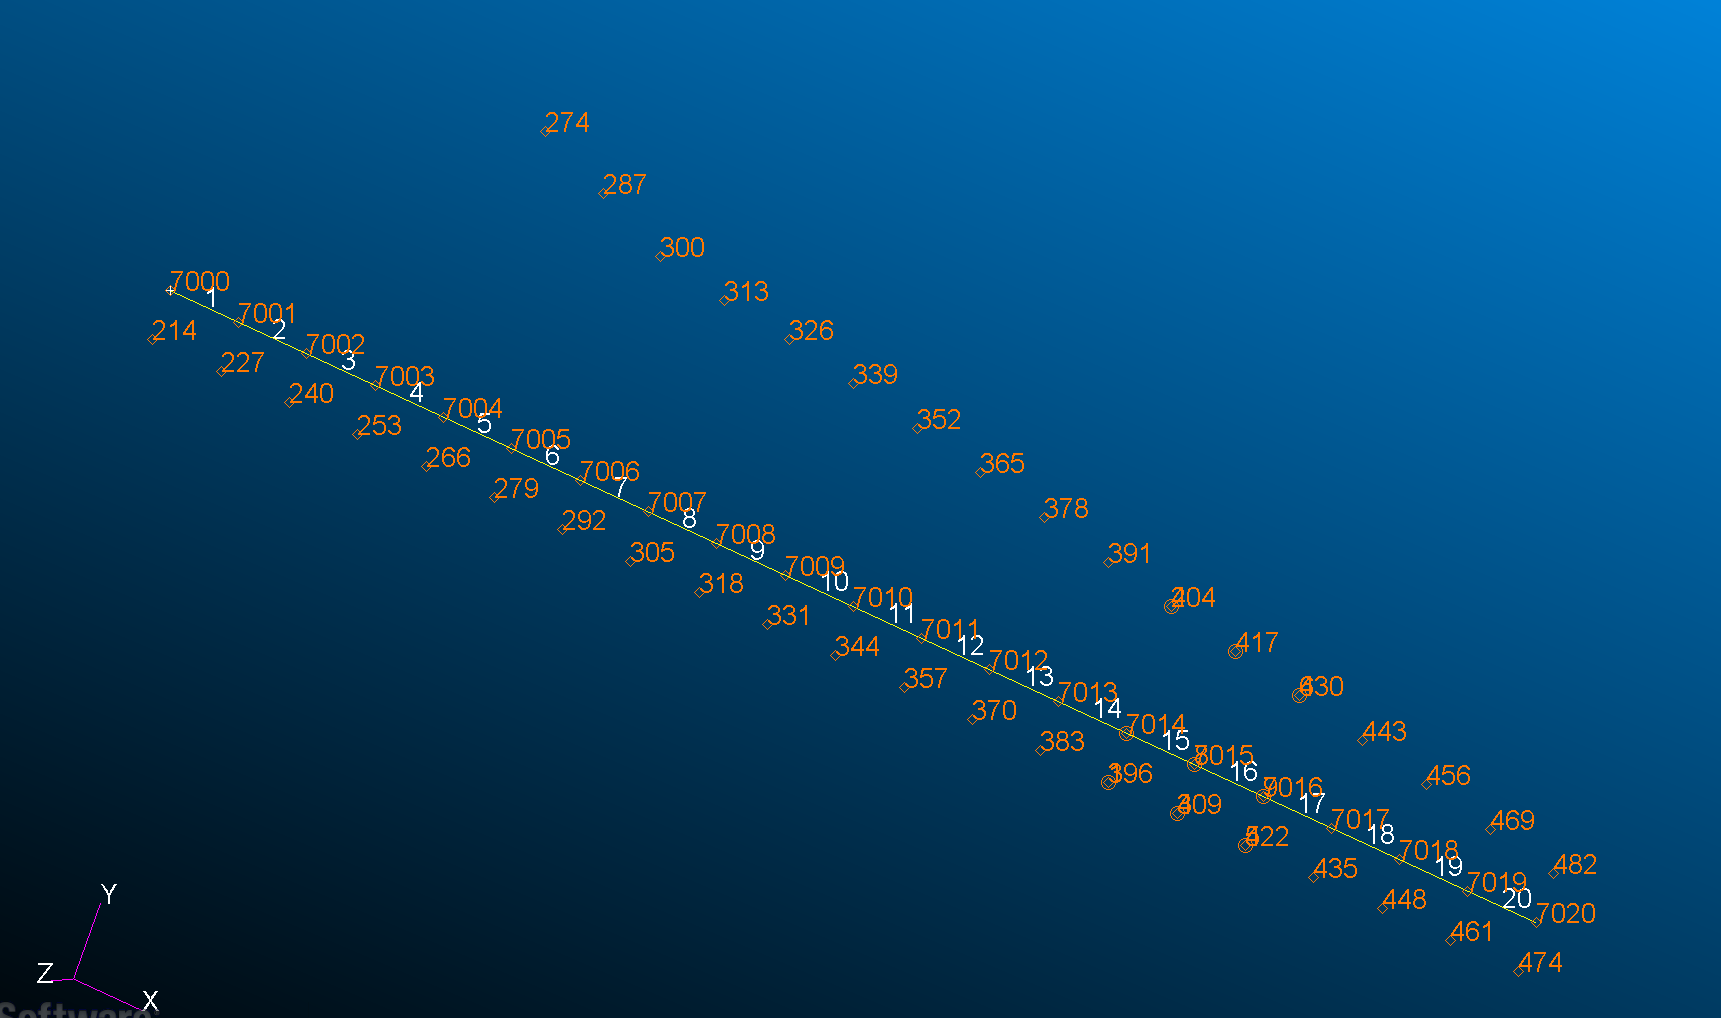
\includegraphics[width = 1\textwidth]{./Immagini/4_17.png}
	\caption{FEM model after new mass distribution implementation}
	\label{fig:4_10}
\end{figure}
In white there are the beam elements used for the stick model, in orange there are the lumped mass used, as u can see for each element, representative of one wing box section, there are 3 lumped mass, one localized on the center of gravity of the element, and two respectively localized on the trailing edge and on the leadng edge.\\
Using this new mass distribution as first we solved the problem related to the torsional modes, then the modal shapes and the frequencies related to the torsional and coupled mode assumed sense value, but there are also improvement on the bending modes. The error on the frequencies for the torsional and coupled mode are now of the same order of magnitude of the errors on the bending mode frequencies, and the last see a reduction of $\approx 5\%$.\\
\newpage 
The new MAC matrix and the new comparison between the frequencies are showed respectively in Fig. \ref{fig:4_11} and in Fig. \ref{fig:4_12}.
\begin{figure}[H]
	\centering
	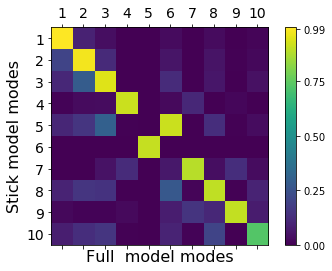
\includegraphics[width = .8\textwidth]{./Immagini/4_15.png}
	\caption{Improvements on the MAC matrix after correction}
	\label{fig:4_11}
\end{figure}
\begin{figure}[H]
	\centering
	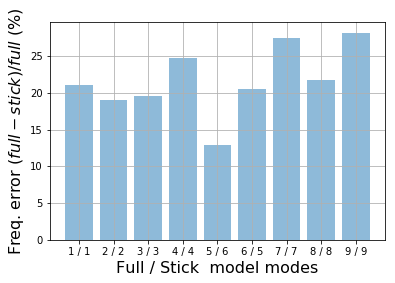
\includegraphics[width = .8\textwidth]{./Immagini/4_16.png}
	\caption{Improvements on the bar frequencies plot after correction}
	\label{fig:4_12}
\end{figure}
\newpage
In Tab. \ref{tab:t2} are showed the new frequencies for the stick model after correction and the relative errors:
\begin{table}
	\begin{tabular}{cccc}
		\toprule
		$Mode $  &  $Full\  model freq. [Hz]$  &  $Stick\  model freq. [Hz]$ & $Relative \ error [\%]$ \\
		\midrule
		$1$  &  $0.73553$  &  $0.55505$ & $ 21.0668$\\
		$2$  &  $2.46789$  &  $1.92782$ & $ 19.0021 $\\
		$3$  &  $5.4666$  &  $4.33701$  &$  19.6497$\\
		$4$  &  $7.66535$  &  $13.3805$ &$ 24.7905 $  \\
		$5$  &  $9.40136$  &  $8.16675$  &$ 12.9799 $\\
		$6$  &  $9.50287$  &  $7.64263$  &$ 20.6029 $\\
		$7$  &  $13.2508$  &  $22.4217$  &$ 27.5247   $\\
		$8$  &  $14.4031$  &  $11.7250$  &$21.778 $\\
		$9$  &  $19.613$  &  $21.4223$  &$28.2195  $\\
		$10$  &  $20.0155$  & $16.4092$ &$ 23.1296$ \\
		\bottomrule
	\end{tabular}
	\caption{Frequencies of full and stick model and relative error after correction}
	\label{tab:t2}
\end{table} 
\subsection{Automatization of the Mode Pairing }
Another problem of the reduction method was the non completely automatization of the process, that doesn't allow an implementation in the optimization process. In fact as we said, when the error on the frequencies is bigger than the step of two frequencies in the row, the order of the mode is not the same for the full and the stick model. Can happen that the 4th mode for the full model is the 1st torsional mode while for the stick model the 4th mode is the 3rd bending mode. Now for a correct evaluation of the errors on the frequencies and the relative correction the errors should be evaluate on the same mode, and the vector of frequencies need to be reorganized. This operation was did manually, by watching the modal shapes using a vizualization software for the output files. \\
To automatize the process we create an algorithm, based on the evaluation of the MAC matrix, to order the vector of frequencies related of the MAC value. In particular blocked the vector of the frequencies related to the full model, we put for each mode the frequencies related to the mode which have the maximum value of MAC, by exploring the full MAC matrix.\\
Once this function was implemented the reduction model could be implemented in the optimization loop to reduce the computational cost of the aeroelastic coupling loop.
\section{Results}
The main objective of this chapter is to prove that the stick model is reducing the overall time of the procedure and can be used for complex and multidisciplinary computations. Thus, in each component a timer was placed in order to calculate the time reduction of the stick model. Certainly, in the first iterations the advantage of the stick model will not be evident since there are two additional components in comparison with the 3D model, thus, extra time. However, when the process reaches the multidisciplinary analysis(MDA), the computational efficiency of the stick model should be clear. \cite{bru}\\
In Tab. \ref{tab:t3} the time cost of each component in both optimizations are presented:
\begin{table}
	\begin{tabular}{l|rr|r}
		\toprule
		$Component $  &  $Full\  model [s]$  &  $Stick\  model [s]$ & $Reduction [\%]$ \\
		\midrule
		$Geometry$  &  $7.97$  &  $7.81$ & $ -2.01$\\
		$Interpolation$  &  $0.371$  &  $0.416$ & $ -88.79 $\\
		$Total\  Reduction$  &  $-$  &  $7.27$  &$  -$\\
		$Aero$  &  $7.26$  &  $7.25$ &$ -0.28$  \\
		$Load\  Transfer$  &  $0.0044$  &  $0.00183$  &$ -58.41 $\\
		$Structure$  &  $3.52$  &  $2.19$  &$ -37.78$\\
		$Displacements \ Transfer$  &  $0.00166$  &  $0.000605$  &$ -63.55   $\\
		$Total\ Pre-MDA \ Process$  &  $8.341$  &  $15.1216$  &$81.29 $\\
		$Total\ MDA\ Process$  &  $10.78606$  &  $9.432435$  &$-12.55  $\\
		$Total\ Time$  &  $116.2016$  & $107.7537$ &$-7.27$ \\
		\bottomrule
	\end{tabular}
	\caption{Time reduction of the stick model}
	\label{tab:t3}
\end{table} 








%
\chapter{Test Cases} 
\label{chapter5}
To validate the optimization script, several test cases have been done.
% Diversi aspetti del problema si sono dovuti testare, al fine di ottenere informazioni sull' effettivo funzionamento del programma, nonchè al fine di far emergere errori e complicazioni non tenute in conto in fase di programmazione. Si sono quindi effettuati test su diversi modelli di ala, in particolare l' ala di Goland e la CRW della NASA, caratterizzati da un livello di dettaglio delle mesh strutturali diversi, noanchè da proprietà aerodinamiche diverse. Inoltre nei vari test si sono usati entrambi i driver scelti per l' implementazione, COBYLA e SLSQP, con i corrispettivi confronti sui risultati; e diverse combinazioni tra objective function and constraints si sono effettutate. 
Many aspects of the problem had to be tested, in order to obtain information on the effective functioning of the software, as well as to bring out errors and complications not taken into account in the programming phase. Tests were therefore carried out on different wing models, in particular the Goland wing and the NASA Common Research Wing CRM , characterized by a different  level of detail of the structural meshes, as well as by different aerodynamic properties. Moreover, in the various tests both drivers chosen for the implementation, COBYLA and SLSQP, were used, with the corresponding comparisons on the results; and different combinations between objective function and constraints were carried out. \\
As first let's see in details the wing model used for the validation of the software.
\section{Goland Wing}
The Goland wing is a wing model developed by M. Goland, and described in \cite{gola}. This model of wing is really simple, and several numerical and experimental studies have been carried out on this wing, which is usually used as reference to validate aeroelastic codes. So for the preliminary approach it's the best choice, because we can obtain fast results and find in literature many works to compare the results.\\
The Goland wing model that we use is based on the model described in the work of Beran P.S. \cite{bera}\\
The wing is schematized as a cantilevered wing. The wing span is 6.10 m, the chord 1.22 m and the thickness 0.51 m.\\
The finite element model is built up from shear panels, modeling the spars and ribs, and membrane elements, modeling the wing skins. The spar and rib caps are modeled by rod elements and posts connect the wing skins at every spar/rib intersection.\cite{sito} In Fig. \ref{fig:5_1} is showed how the initial FEM model is structured.\\
The result is a very flexible wing, that it's ideal to show several aeroelastic behavior.\\
\begin{figure}[H]
	\centering
	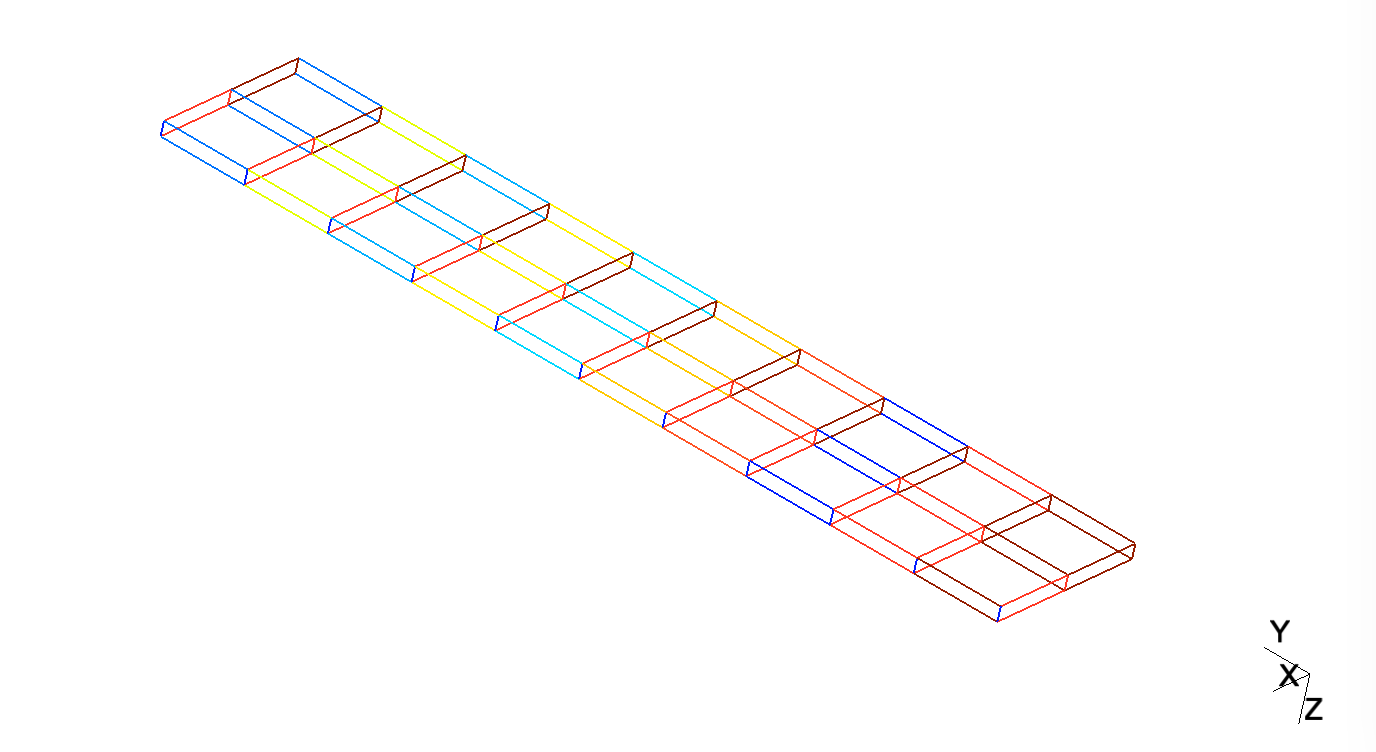
\includegraphics[width = 1\textwidth]{./Immagini/5_1.png}
	\caption{Initial FEM model for the Goland wing}
	\label{fig:5_1}
\end{figure}
For the aerodynamic mesh an airfoil are obtained using a 4\% thick parabolic arc, then the mesh is generated using 4 section until the wing span, for each section several point of the airfoil are considered, with a condensation of nodes on the trailing and leading edge, then the panel are obtained joining the nodes and the sections. In Fig. \ref{fig:5_2} is showed how the initial aerodynamic mesh is structured.
\begin{figure}[H]
\centering
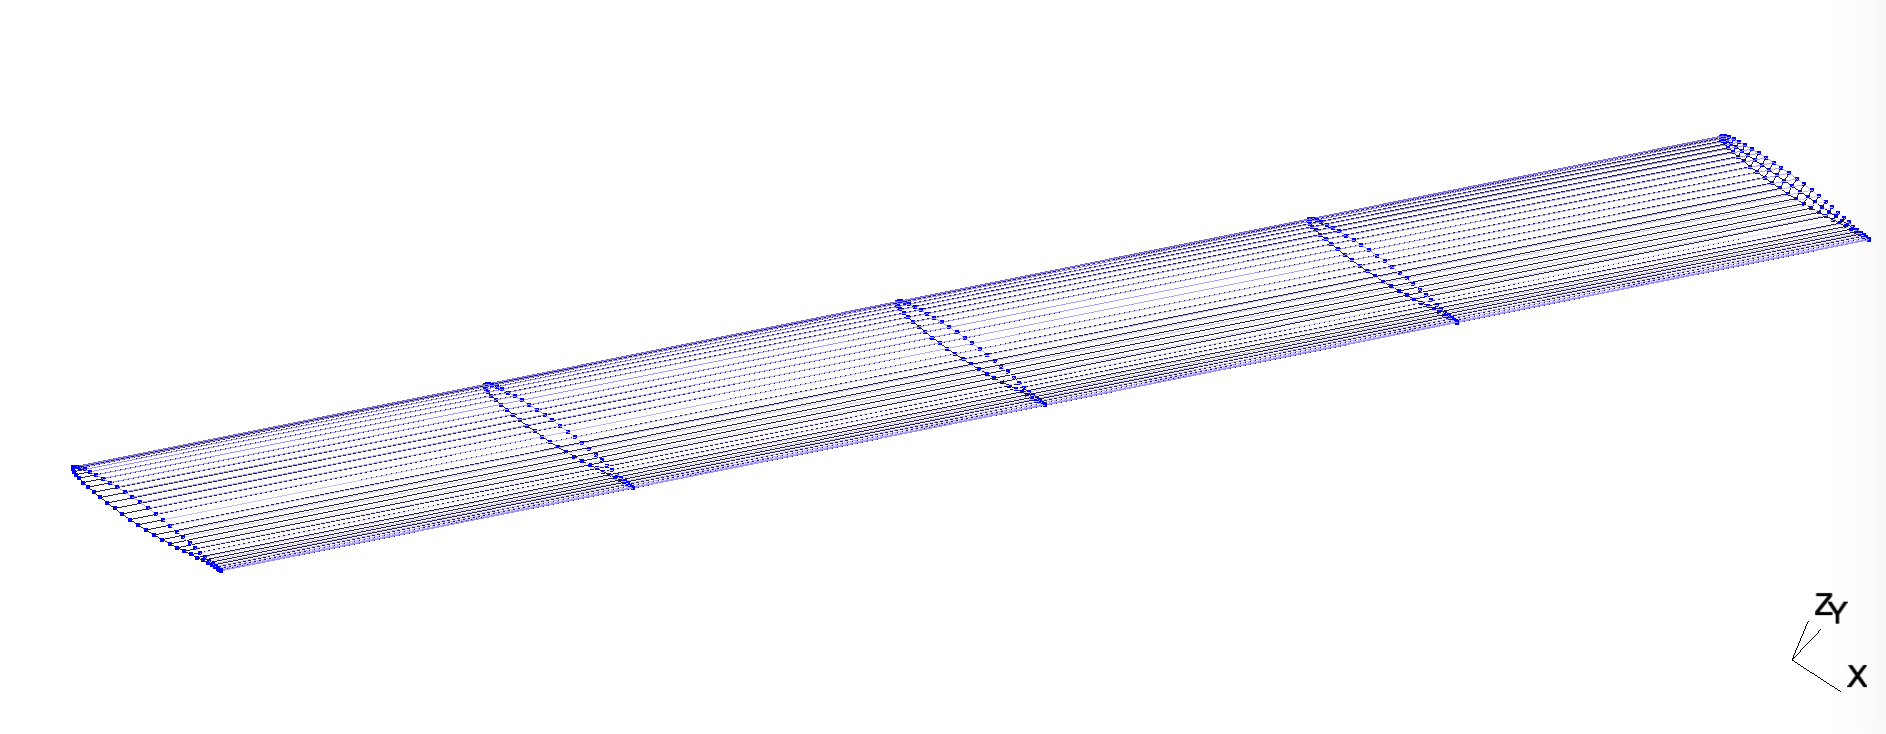
\includegraphics[width = 1\textwidth]{./Immagini/5_2.png}
\caption{Initial aerodynamic mesh for the Goland wing}
\label{fig:5_2}
\end{figure}

\section{CRM wing}
The second wing model used for the test cases is the NASA Common Research Model Wing \textbf{CRM}. This choice has been adopted in order to have a more complex wing's model, to access to more problematic and design's aspect, compared to the Goland wing, and the choice was the CRM, because several project is based on this model, so we can easily find in literature results to compare, and evaluate the quality of them.\\
The Common Research Model (CRM) consists of a contemporary supercritical transonic wing and a fuselage that is representative of a widebody commercial transport aircraft.  The CRM is designed for a cruise Mach number of $M_{\infty} = 0.85$ and a corresponding design lift coefficient of $C_L= 0.5$. \cite{nasa2}\\
The wing consist in a fullscale cantilevered wing. The CRM was generated as open geometry for the research, imagined for transport class aircraft with single-aisle configuration. The geometry of the wing is more complex of the Goland wing, in fact there are sweep angle, taper ratio, etc... .It's caraterized of a wing span of $58.76 \ m$, an aspect ratio of 9, a root cord of $7\ m$, a taper ratio of 0.275, a leading edge sweep angle of $35 \deg$, and a break along the trailing edge at 37\% of the semi-span, the wing reference area is $ 383.68\  m^2$. For the structure the wing box is defined to lie between 10\% and 70\% of the wing cord. 
\newpage
In Fig. \ref{fig:5_3} the plan view of the CRM wing is showed:
\begin{figure}[H]
	\centering
	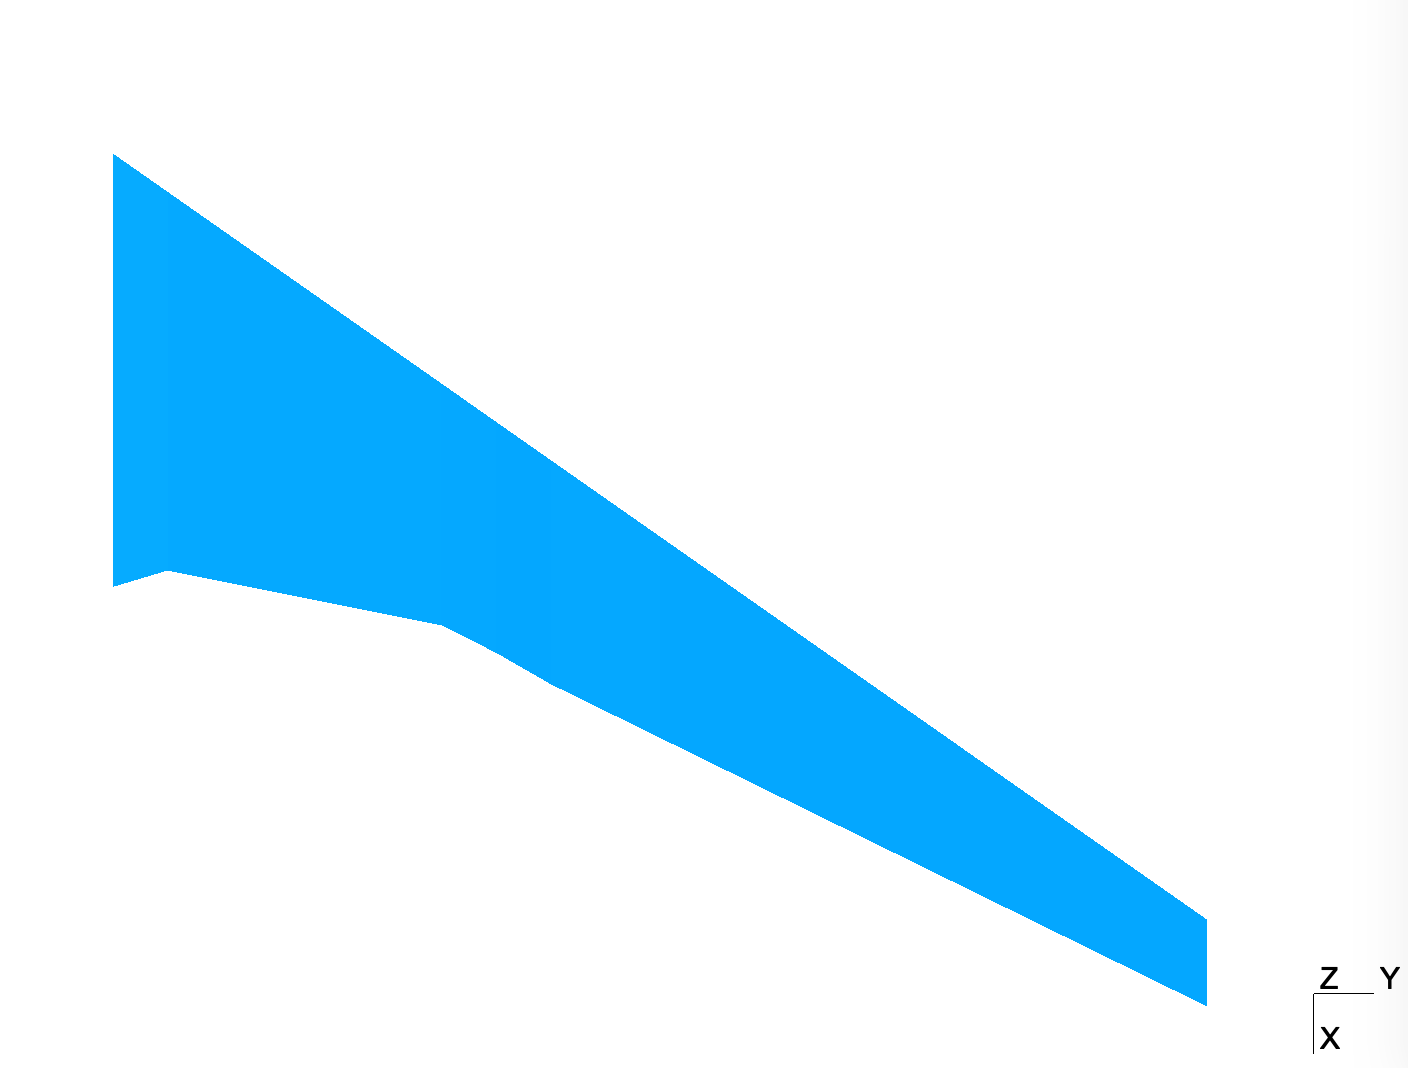
\includegraphics[width = 1\textwidth]{./Immagini/5_4.png}
	\caption{Plan view of the CRM wing geometry}
	\label{fig:5_3}
\end{figure}
For the structural model an high fidelity model have been created. All the component of the wing (ribs, spar, stringer, skin) are modeled using shell elements. Over 25'000 finite elements have been used. In Fig. \ref{fig:5_4} the complete FEM model is showed:
\begin{figure}[H]
	\centering
	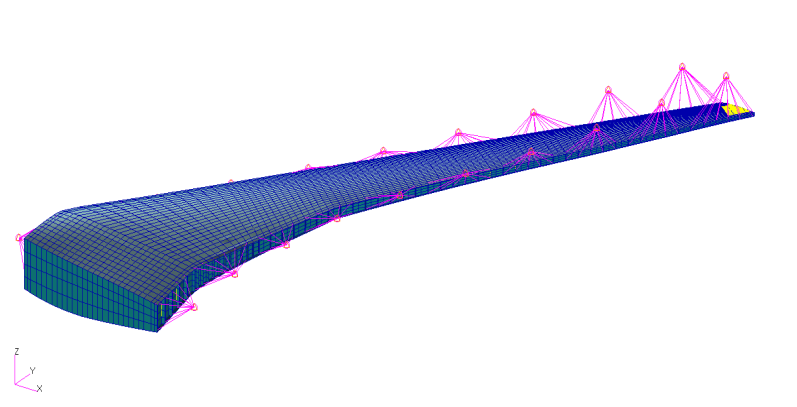
\includegraphics[width = 1\textwidth]{./Immagini/5_5.png}
	\caption{FEM model of CRM wing}
	\label{fig:5_4}
\end{figure}
The airfoil used to obtain the aerodynamic mesh is the CRM-65 in Fig. \ref{fig:5_5}, provided by NASA \cite{air}. The aerodynamic mesh is obtained using 50 different section, in order to take account of the taper ratio and the thickness. In Fig. \ref{fig:5_6} the aerodynamic mesh is showed:
\begin{figure}[H]
	\centering
	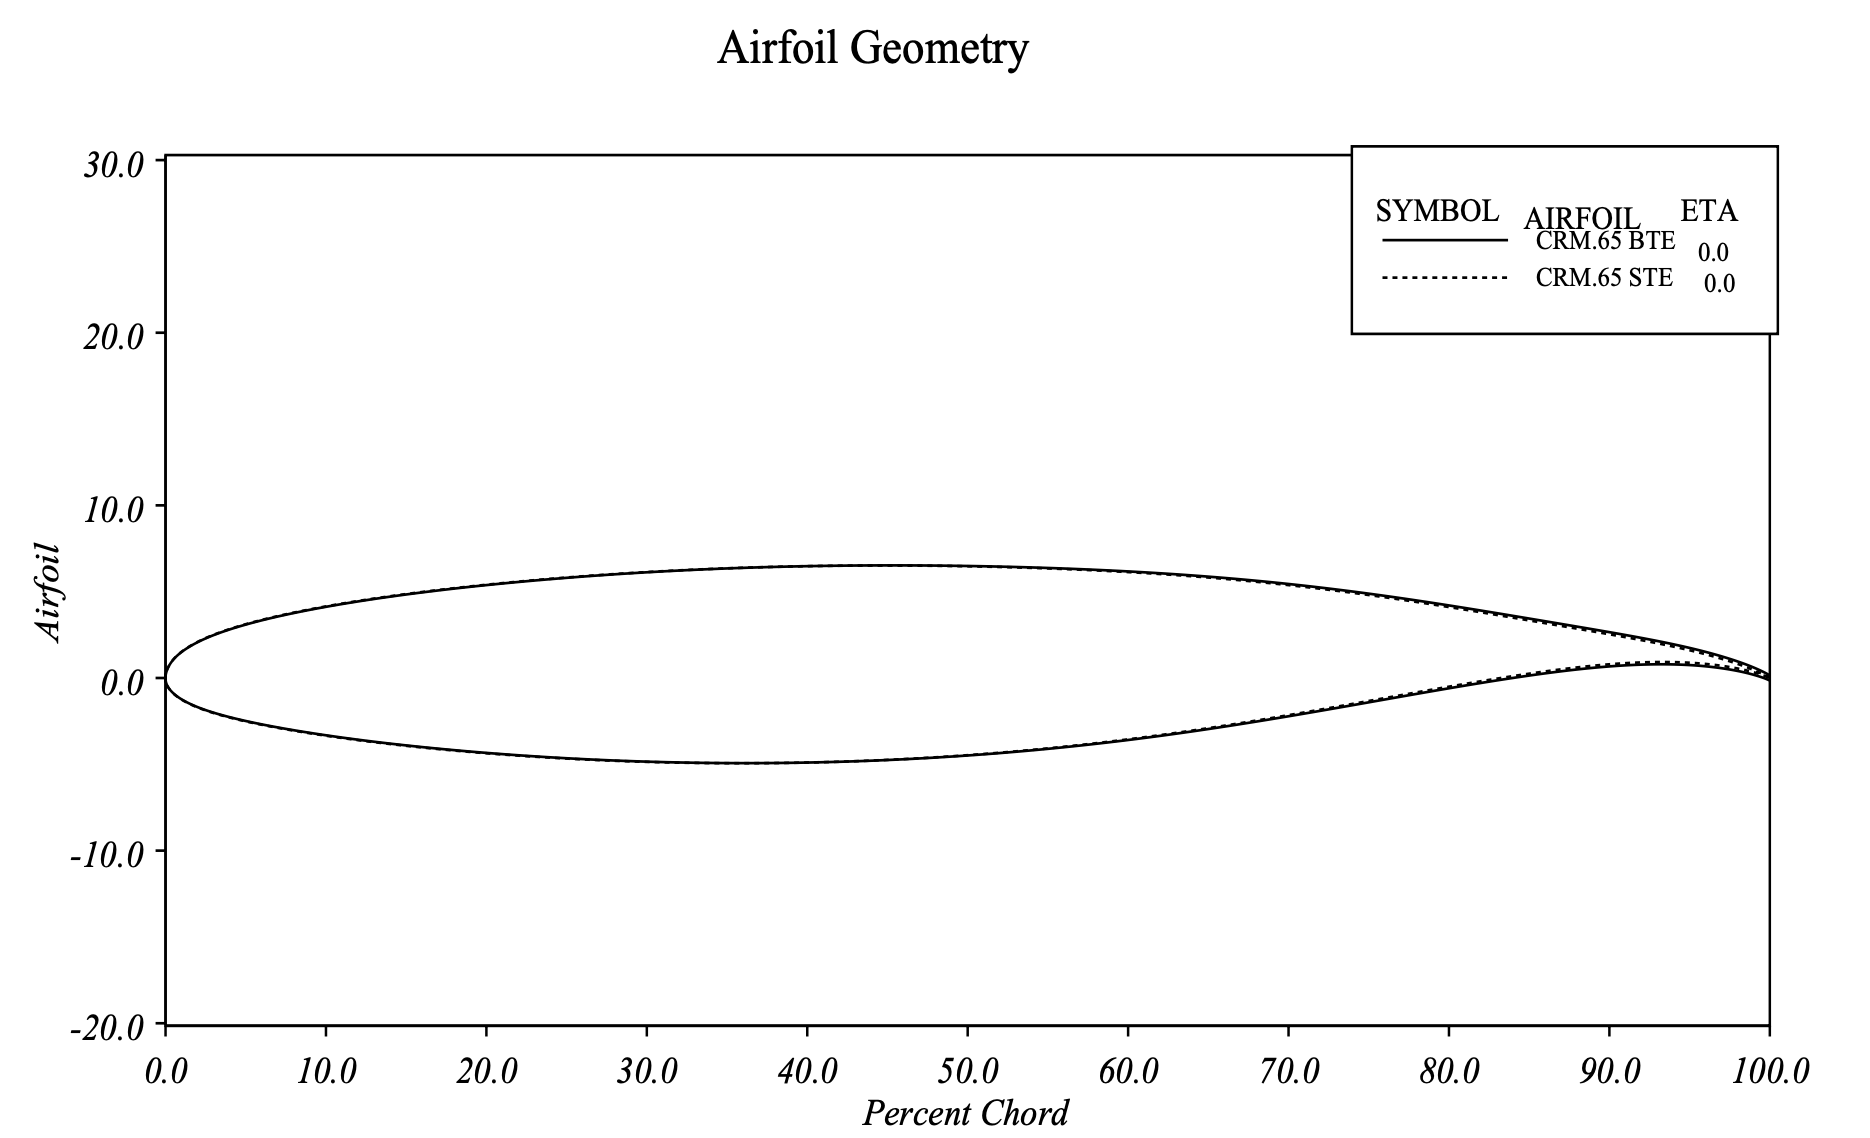
\includegraphics[width = 0.7\textwidth]{./Immagini/5_6.png}
	\caption{CRM-65 airfoil}
	\label{fig:5_5}
\end{figure}
\begin{figure}[H]
	\centering
	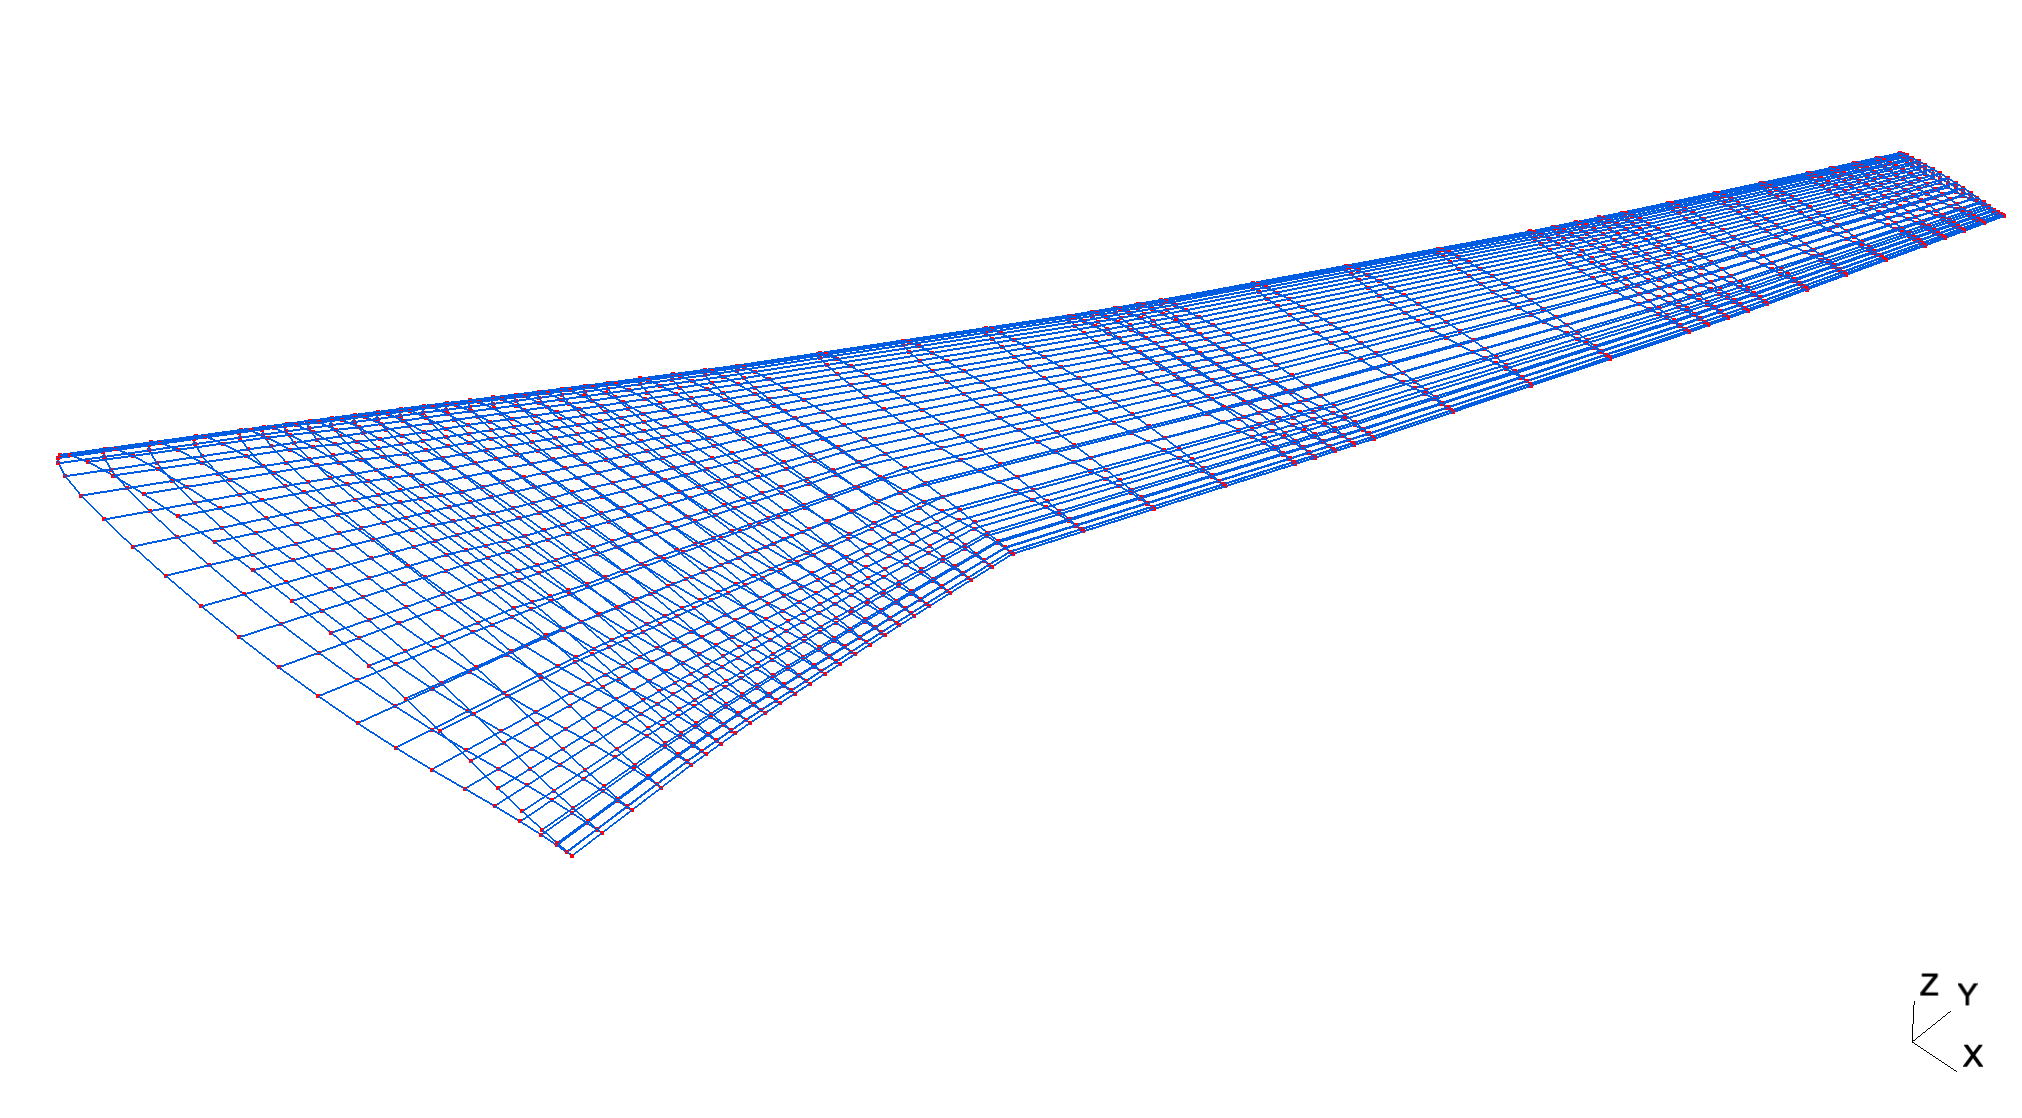
\includegraphics[width = 1\textwidth]{./Immagini/5_7.png}
	\caption{Aerodynamic mesh of the CRM wing}
	\label{fig:5_6}
\end{figure}
\section{CRM Wing Simple Model}
The CRM wing model allow to consider more parameters in the optimization process, but the cost of the structural and aerodynamic analysis for the model that we create are really high. In the test phase of the component, where coding or conceptual errors emerge, the time required to launch the code can be prohibitive. So to solve this problem a simple model of the CRM wing have been used, in order to have all the proprieties of the CRM wing but with a much less computation cost. The quality of the result is, of course, worse, but in that phases we wasn't interested to obtain result, but just to validate the code.\\
The most important changes are on the structural model. As first much less elements have been used, from 25'000 to 1'000, then instead to use shell elements for all the components, beam elements have been used for stringer and spars.\\
In Fig. \ref{fig:5_7} the structural mesh of the simple model of the CRM wing is showed, the beam elements are in red while the shell elements are in blue:
\begin{figure}[H]
	\centering
	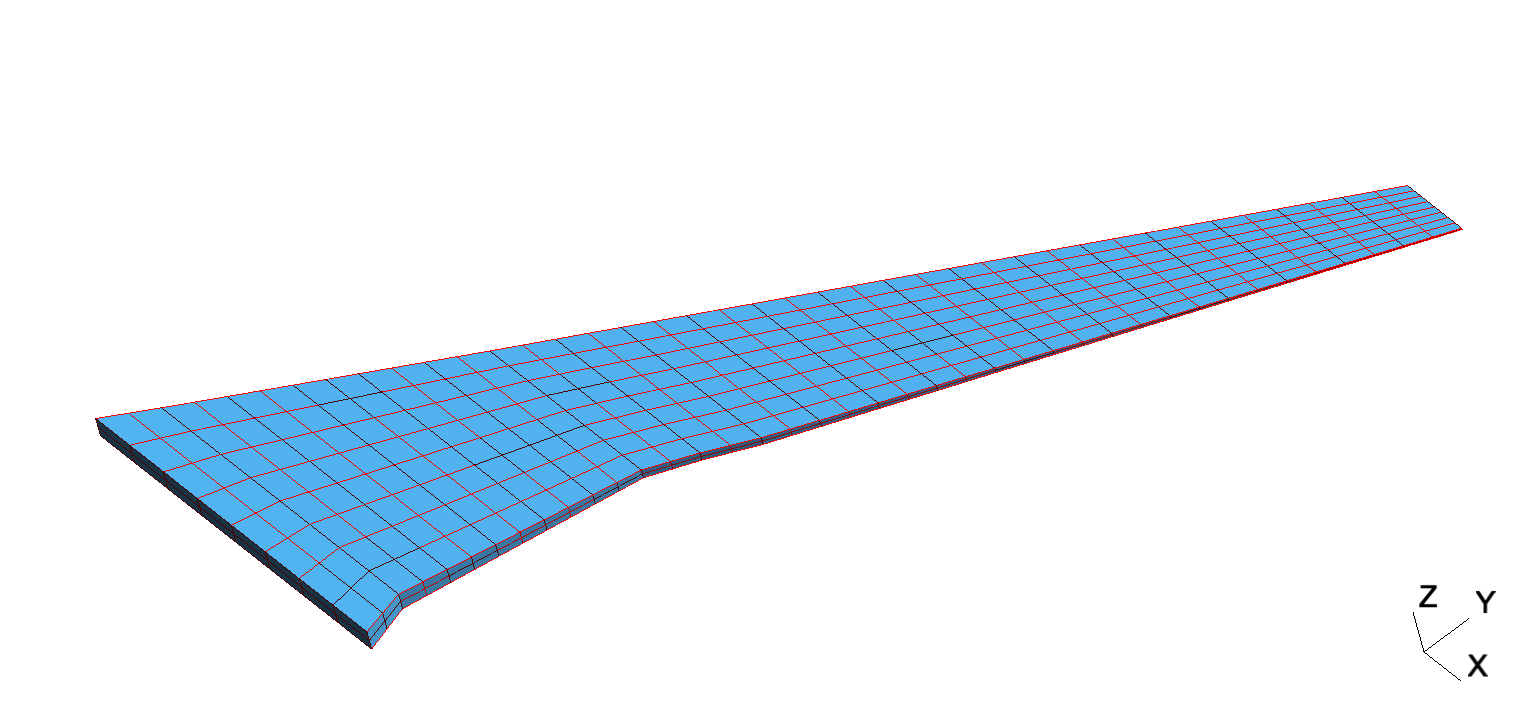
\includegraphics[width = 1\textwidth]{./Immagini/5_8.png}
	\caption{Aerodynamic mesh of the simple model CRM wing}
	\label{fig:5_7}
\end{figure}
Also the aerodynamic mesh is simple. In this case we just reduced the number of section, from 50 to 20. In Fig.\ref{fig:5_8} is showed the aerodynamic mesh of the simple CRM wing model:
\begin{figure}[H]
	\centering
	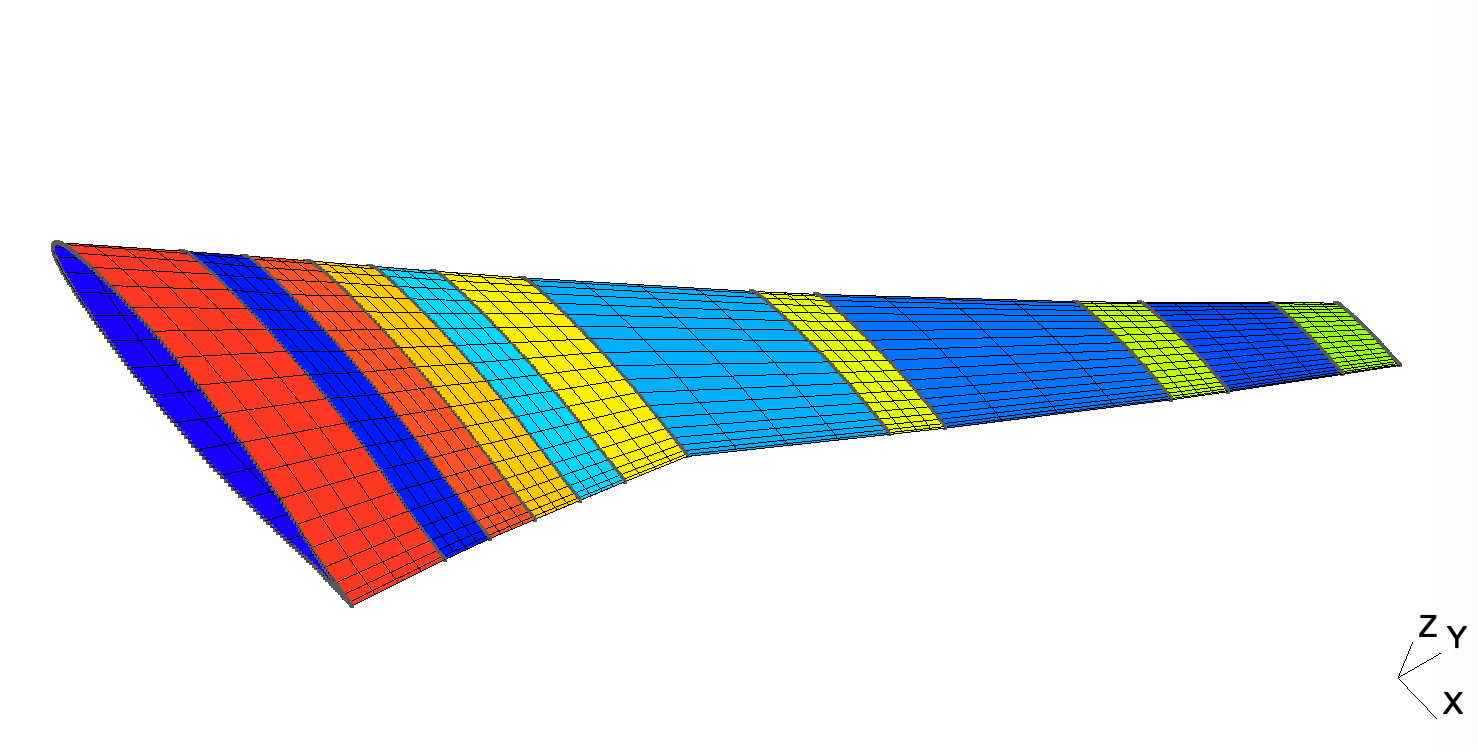
\includegraphics[width = 1\textwidth]{./Immagini/5_9.png}
	\caption{Aerodynamic mesh of the simple model CRM wing}
	\label{fig:5_8}
\end{figure}
\section{Different Options for the Optimization}
Several test cases have been performed in order to validate the different components, to test the different drivers, the different wing model. So each test case represent a combination of different option and has different goal. In Tab. \ref{tab:t4} there are collect all the possible option used in the various test case:
% Please add the following required packages to your document preamble:
% \usepackage{multirow}
% Please add the following required packages to your document preamble:
% \usepackage{multirow}
\begin{table}[H]
	\centering
	\begin{tabular}{c|c}
		\hline
		\textit{Options}                                                               & \textit{Possible Choice}            \\ \hline
		\multirow{3}{*}{Wing Model}                                                    & Goland Wing                         \\
		& CRM Wing                            \\
		& CRM Wing Simplified                 \\ \hline
		\multirow{2}{*}{Driver}                                                        & COBYLA                              \\
		& SLSQP                               \\ \hline
		\multirow{4}{*}{\begin{tabular}[c]{@{}c@{}}Design\\ Variables\end{tabular}}    & Angle of Attack $\alpha$            \\
		& Thickness of Shell Elements         \\
		& Sweep Angle $\Lambda$               \\
		&  Wingspan $b$                                   \\ \hline
		\multirow{3}{*}{\begin{tabular}[c]{@{}c@{}}Objective\\  Function\end{tabular}} & Mass $m$                            \\
		& Induced Drag Coefficient $C_{D_i}$  \\
		& Generic Function $f$                \\ \hline
		\multirow{3}{*}{\begin{tabular}[c]{@{}c@{}}Generic \\ Options\end{tabular}}    & Constraint Aggregation              \\
		& Design Varibles Limit as Constraint \\
		& Reduced Structural model            \\ \hline
	\end{tabular}
\caption{Different option selectable for the optimization}
\label{tab:t4}
\end{table}
\section{Problems}
During the test cases several problems emerge. In this section we will explain the most relevant problems, and the relative solution that we find. 
\subsection{Cobyla Design Variables Limits}
One of the first problem that have emerged when we pass to the CRM wing cases was relative to the use of the optimization driver COBYLA. The problem was that when the thickness of the wing tip shell elements, the zone of the wing characterized to the biggest value of displacements , start to be to little, the displacements start to being really impressive. Then this displacements are moving into the aerodynamic mesh using the interpolation. Now if the wing tip section nodes are moving too much, the aerodynamic analysis will fail, because the mesh assume a weird shape. That's cause the crash of the program and interrupts the optimization. The direct consequence is to set limits for the design variables, in this case limits on the minimum value of the shell elements thickness, in order to avoid that the displacements being huge. Then we set limits on the thickness as $10^{-3}\ m$.\\
Using the COBYLA optimization we see that, despite the design variables limits was exactly set, the optimization still crash. Then opening the database of the iterations we saw that the limits of the design variables are not respected, as we can see in Fig. \ref{fig:5_9}:
 \begin{figure}[H]
 	\centering
 	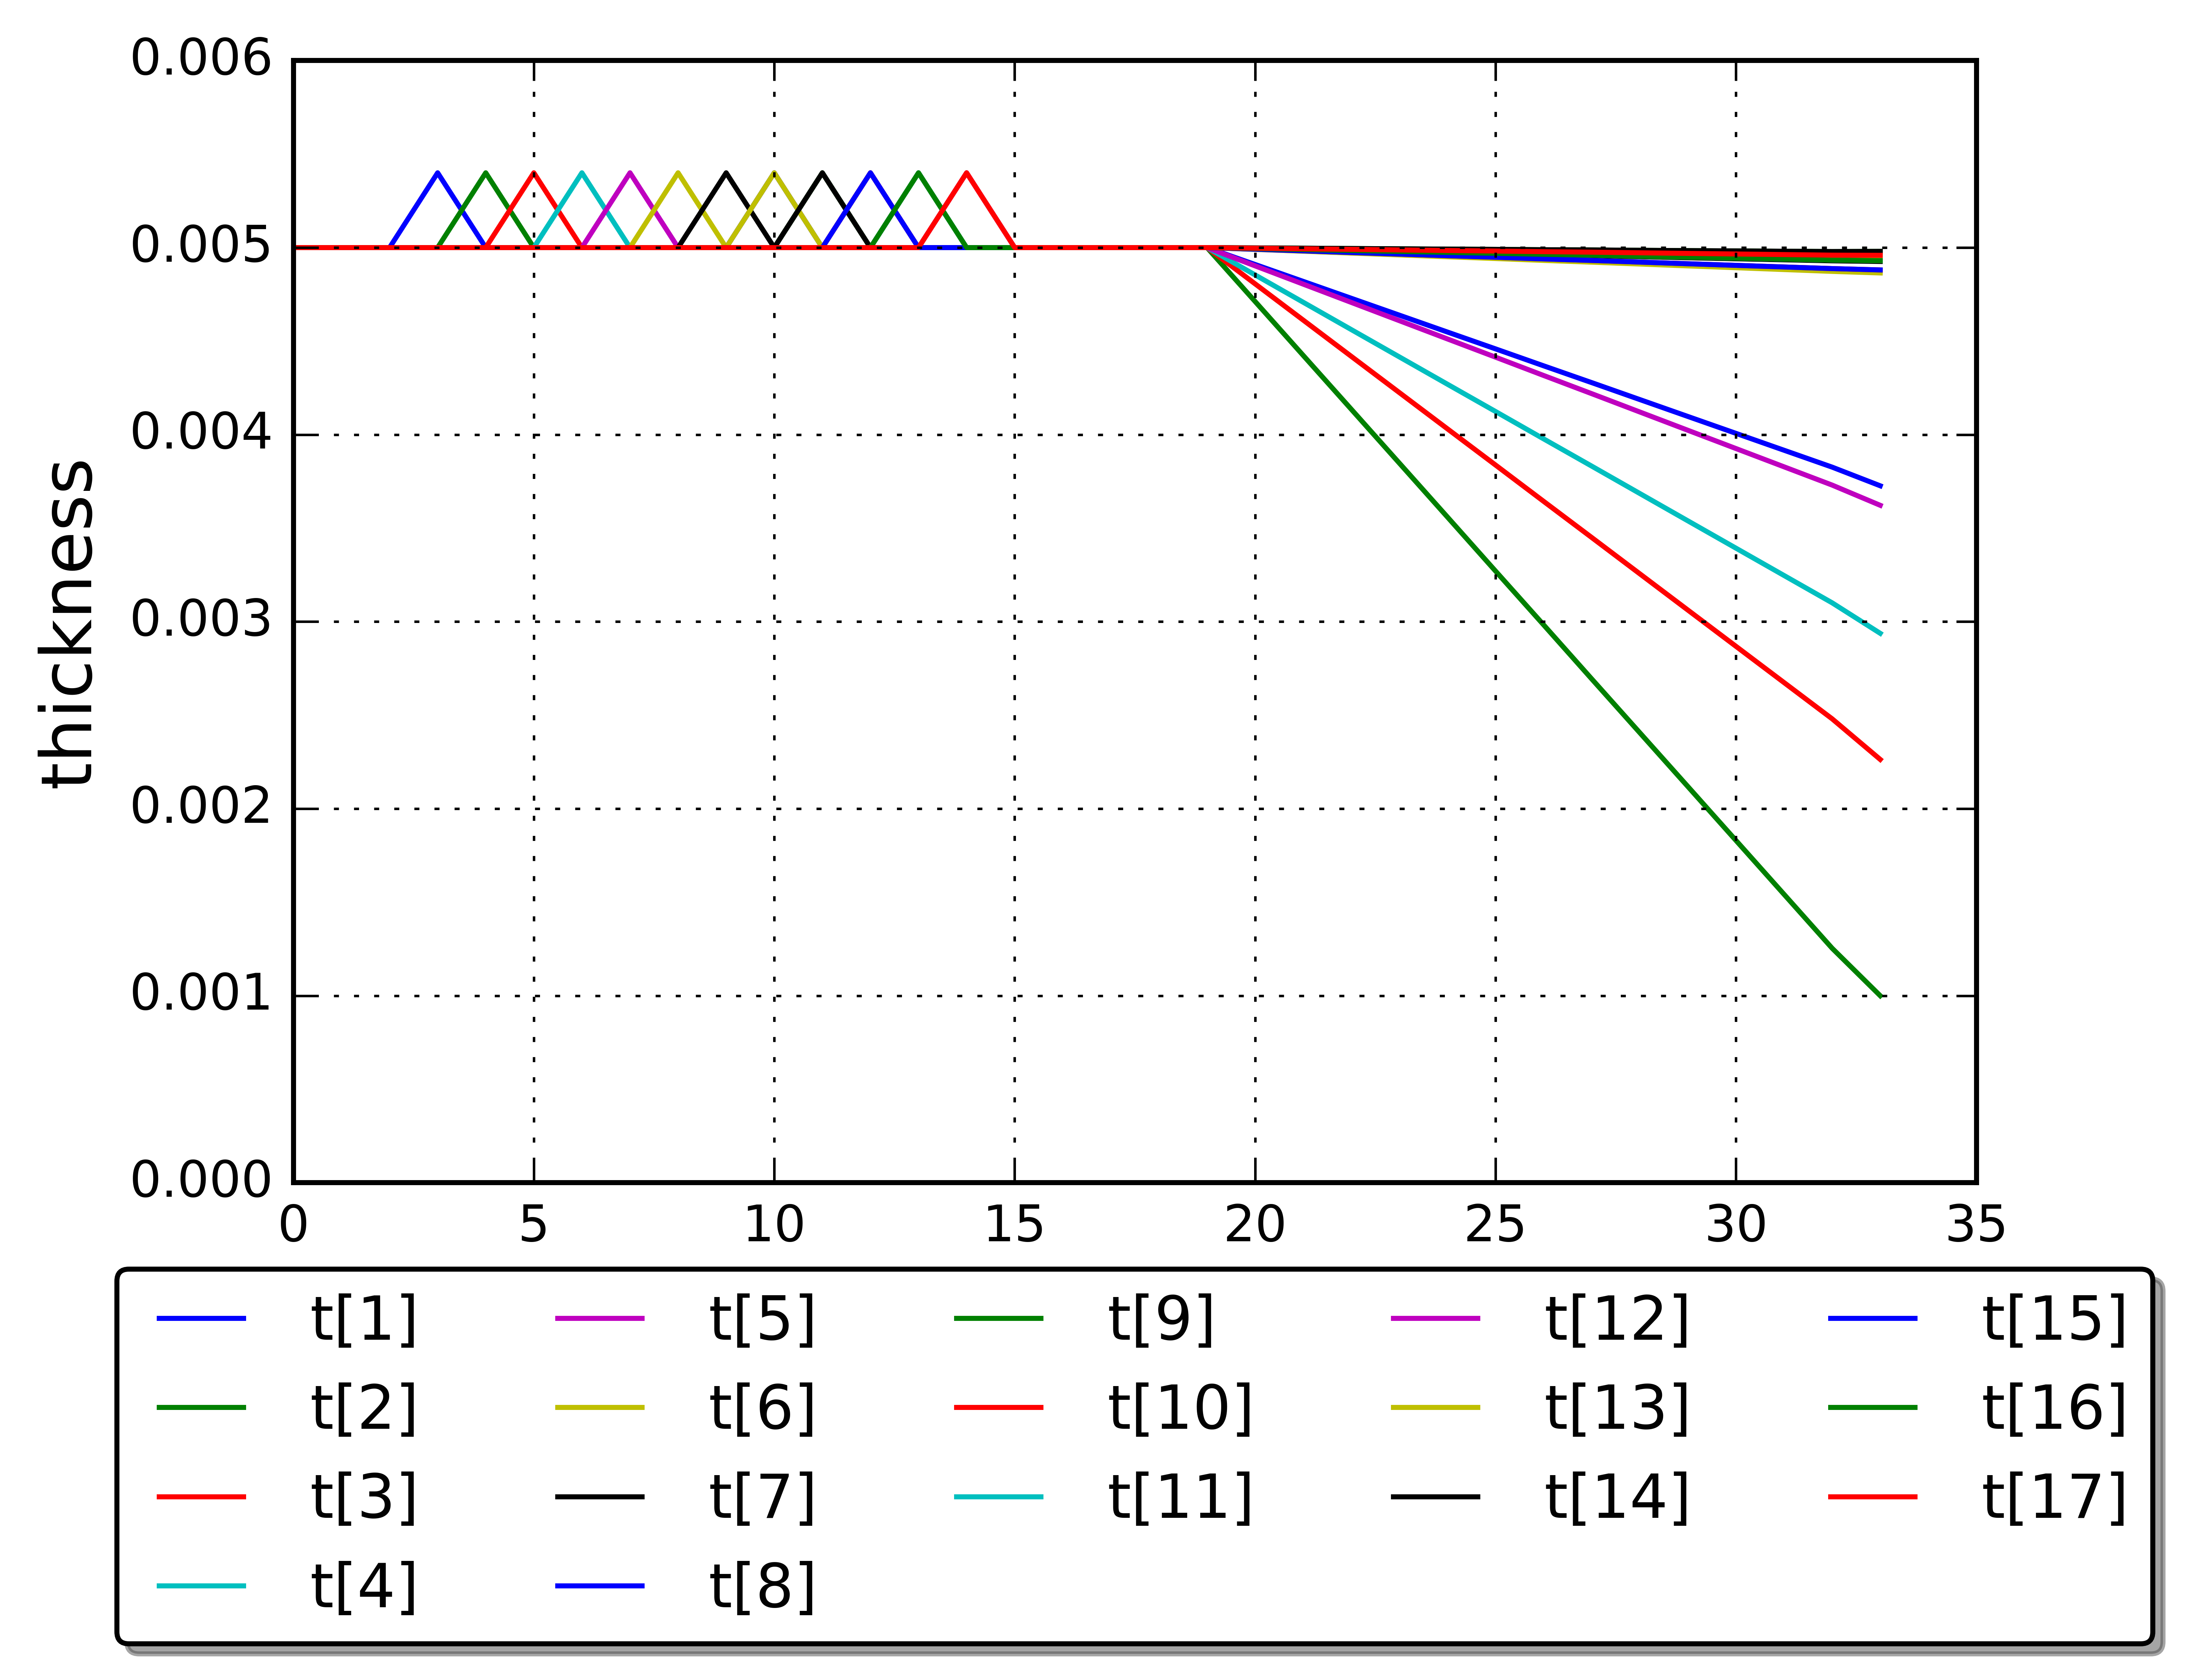
\includegraphics[width = 0.8\textwidth]{./Immagini/5_10.png}
 	\caption{Thickness variation in a COBYLA optimization}
 	\label{fig:5_9}
 \end{figure}
As we can see the optimization crashes at the iteration 34, because the thickness of the section 16 is lower than $10^{-3}\ m$. The problem is that COBYLA doens't respect the design variables limits. That's is result of the is a consequence of how it was programmed, COBYLA is a driver programmed to get results, so when it decide the direction of the optimization, in this case the direction is to reduce the thickness of section in order to obtain a reduction of the mass of the wing, it still work in order to get the convergence of the objective function respecting the constraints. \\
To solve this problem, and avoid the crashes, our solution was to set also the thickness limits of the section as constraint, in order to be respected by COBYLA. So a new set of constraint have been created, the constraints equation check for each iteration if the minimum value of the thickness is bigger than the limit which we set:
\begin{equation*}
con(t_i)=t_i-t_{i_{min}} >0 \qquad i=1,2,...,n_t
\end{equation*}
where $con(t_i)$ is the constraint function, $t_i$ the value of the thickness of the section $i$, $t_{i_{min}}$ the limit of the thickness and $n_t$ the number of the section with different thickness.\\
In order to check if the solution works, we start a particular optimization focused on the reduction of the thickness for all the section, and check if the limits on the thickness if finally respected, as is showed in Fig. \ref{fig:5_10}:
 \begin{figure}[H]
	\centering
	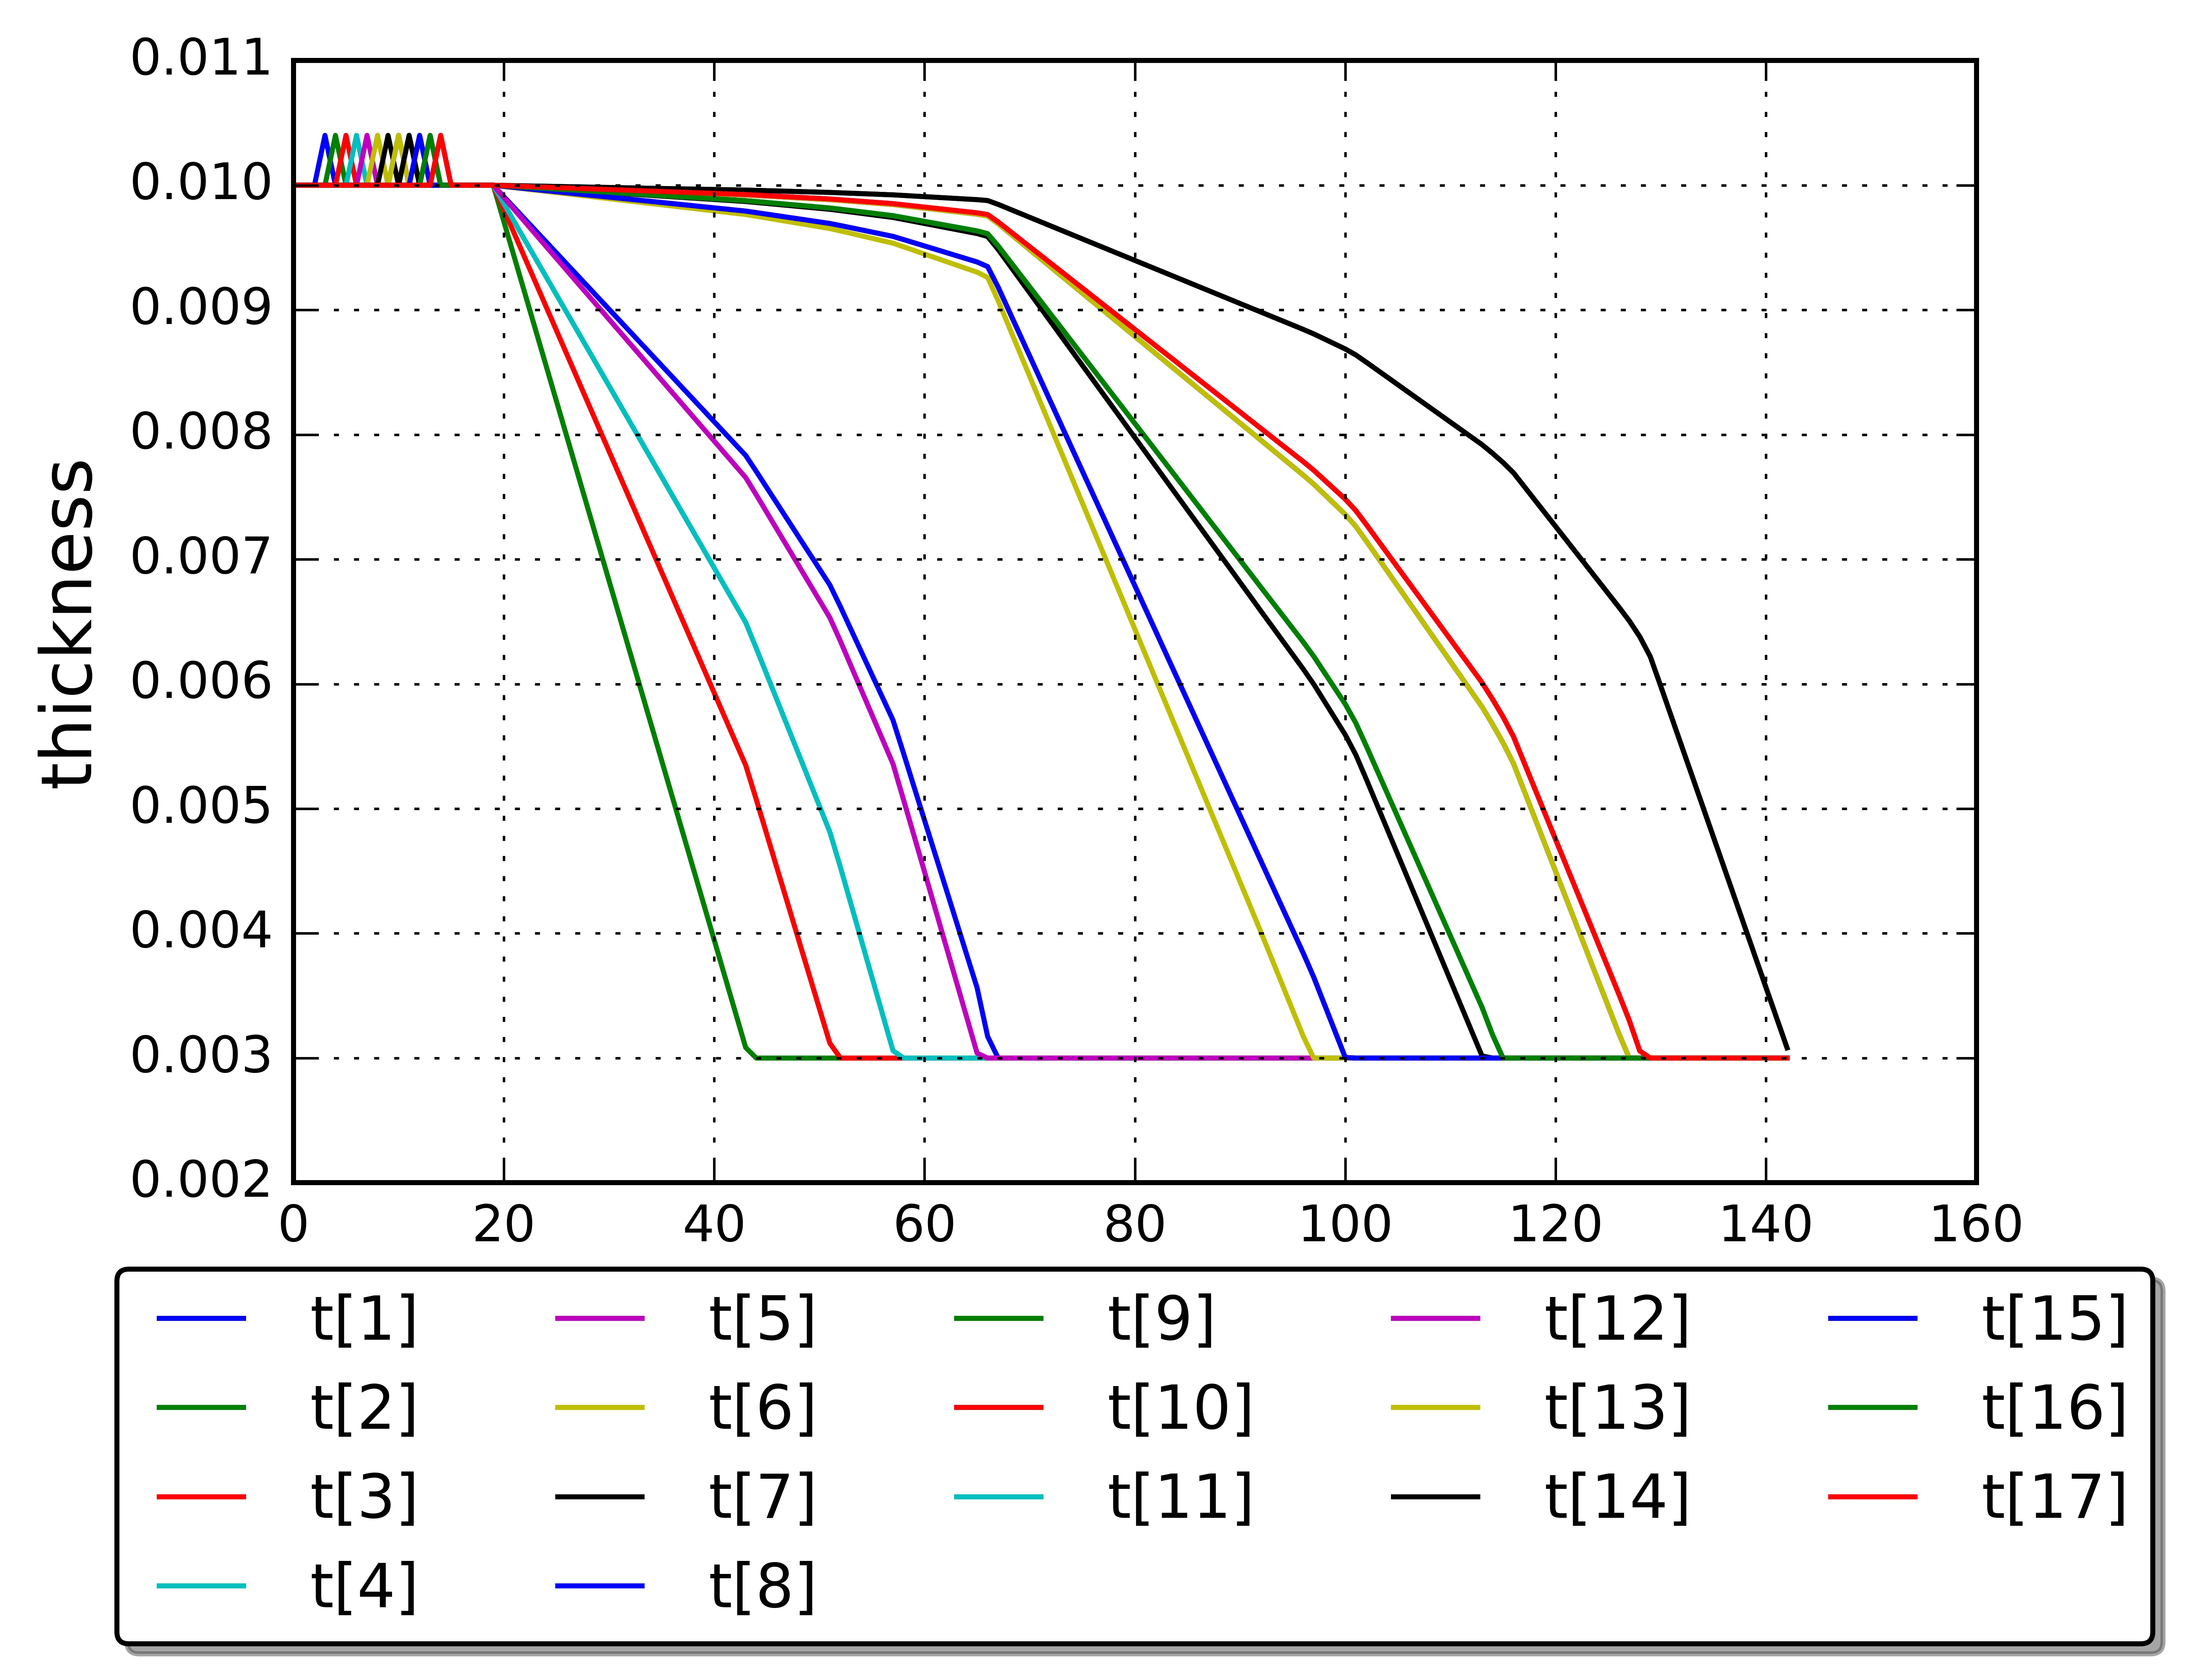
\includegraphics[width = 0.8\textwidth]{./Immagini/5_11.png}
	\caption{Thickness variation after design limits correction}
	\label{fig:5_10}
\end{figure}
As we can see the correction works well, in fact when the thickness reach the design limit, in this case $3*10^-3$, that value will not more changed, and the stability of the optimization is guaranteed.
\subsection{Finite Difference Gradient Evaluation Error }
Another error has emerged using the SLSQP driver. As we said in the chapter 2, to evaluate the gradient, for the gradient based optimization using SLSQP, we use the finite difference method. In our specific case one of the gradient that we need for the optimization, being the thickness of the section a design variables, and the Von Mises stress a constraint, like the lift, and the mass an objective, the gradient of these function respect to the thickness.\\
As we explain the structural analysis and the aerodynamic analysis is performed by the external codes, respectively NASTRA95 and Panair. So to compute the gradient the flow-chart is the following, for example in the case of the gradient of the mass respect the thickness:
\begin{enumerate}
	\item Set the the starting value of the thickness
	\item Perform an static structural analysis
	\item Extract from the output file the value of the mass
	\item Change the thickness of the finite difference step
	\item Perform an static structural analysis
	\item Extract the new value of the mass from the output file
	\item Compute the gradient using the finite difference equation
\end{enumerate}
The problem that we found was that using the default settings, the solver can't evaluate the gradient, as the mass didn't change after a change of the thickness. That happens because NASTRAN95 use a 8 bit floating point numeration; so the finite difference step set as default for SLSQP is $10^-4$, so the effect that the variation of this step induce on the structural mass is really little, and it changes just the 9th or 10th significant digits, then NASTRAN95 cut the information after the 8th significant digit, so he will lose the information on the variation of the mass, and the mass seems unchanged.\\
To solve this problem is just necessary to specify in the setting of the driver the new step used for the finite difference, in order to induce a bigger variation on the structural mass, then the information on the variotion of the mass will not lose, in our case a step of $10^-2$ it's enough to compute correctly the gradient.
\subsection{Nastran Output File Reader}
Another problem emerged in the test cases is relative to the structural component, specifically for the output file reading method. In order to extract the information of the Von Mises stress for each element we set NASTRAN95 to save this information in a \textit{.pnh} file, characterized by a special structure of the file. Then the structural component after the analysis access to this output file, and an algorithm have been written to associate all the stress to the elements and save these information in a python dictionary. The algorithm have been written in relation at the output file of an analysis performed on the CRM wing, where only shell elements have been used. In the moment that we introduce the simple CRM wing model that contains also beam elements, the structure of the output file changes, then the algorithm can't read successfully it. In the first moment a new algorithm have been written to read correctly also the new output file, but we are working in order to make it universally. The idea is to use an \textit{.exe} file that convert the \textit{.pnh} file. The difference between the output files is that the number of the stresses depends on the number of the degree of freedom of the elements, then the data is collected on more lines. The \textit{.exe} file is structured to convert the file in a file where all the stress of one element are collected on just one line, then is easy to write an algorithm to collect the data independently of the wing structural model chosen. 


\chapter{Results} 
\label{chapter6}
In this chapter are collected the results related to the most significant test cases. For each case all the combination of the setting used have given, together with the graph relative to the trend of the design variables, constraints and objective function until the iteration. The data relative to this trend are collected in a database, created using the recording function implemented in the openMDAO package. So to access to te result is required to use the openMDAO database function, for this reason an external component have been created in order to access to the database and plot the graphics.
\section{Reader code}
In order to collect all the information through the optimization process, the recorder function of openMDAO have been used. This function provide to create a database, which contain all the value of the variables. For each iteration a new dictionary will be created, this dictionary contain one dictionary for each type of variables, in the last there are all the value of the variables for that iteration, as showed in Fig. \ref{fig:6_1}:
\begin{figure}[H]
	\centering
	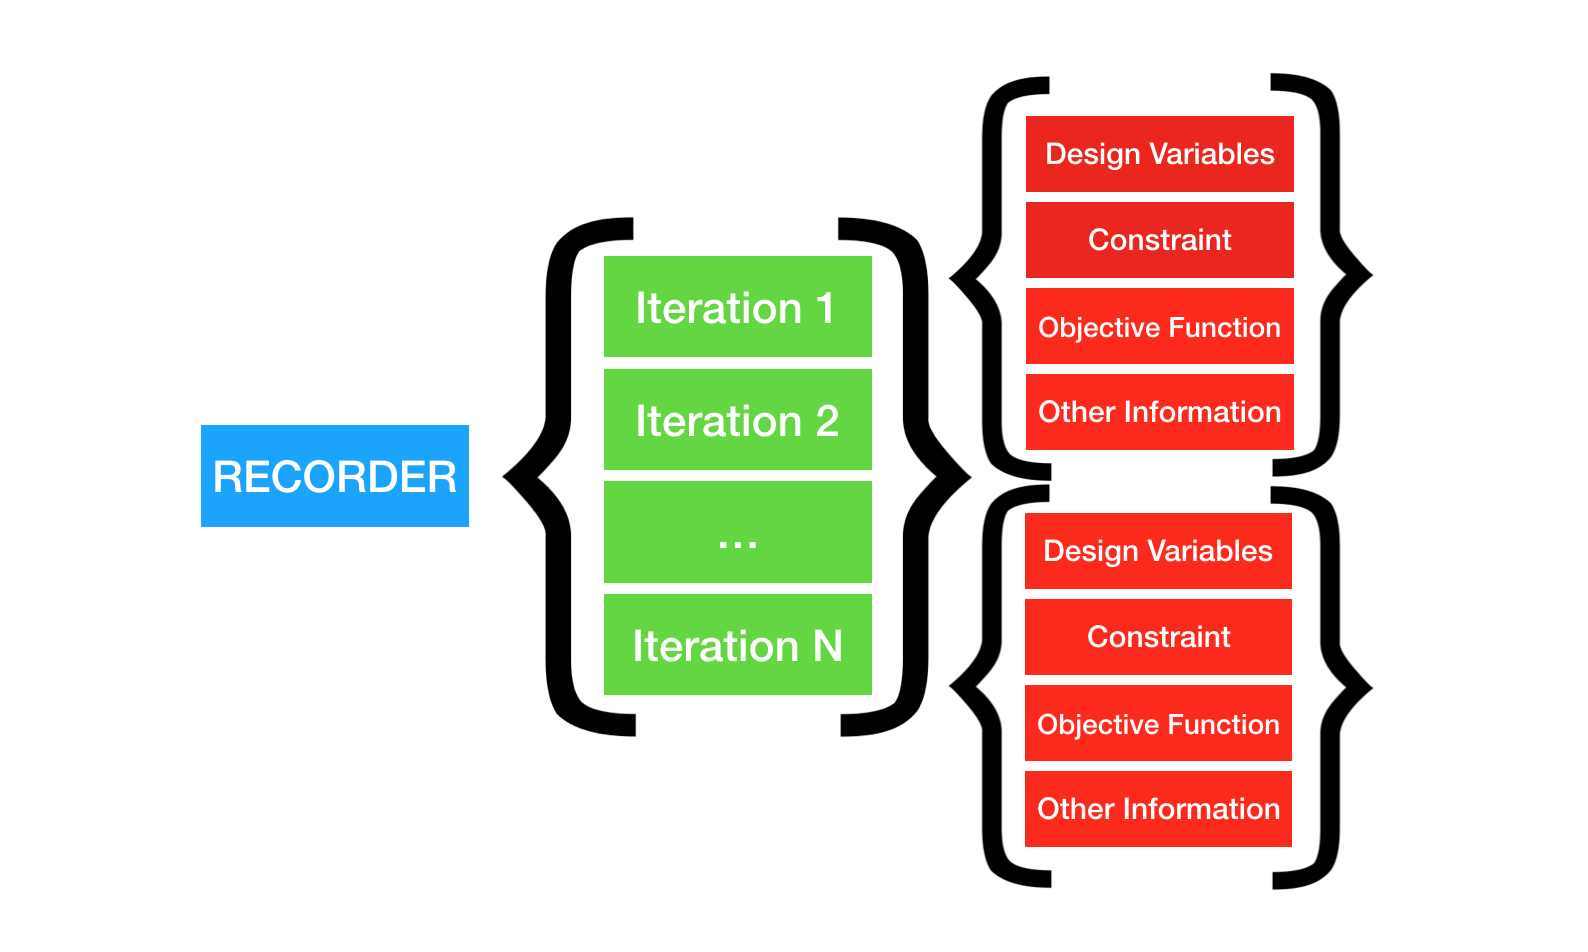
\includegraphics[width = 0.8\textwidth]{./Immagini/6_1.png}
	\caption{Structure of the recorder output file}
	\label{fig:6_1}
\end{figure}
Since the database file name is set, is possible to extract the keys of the dictionary, which are representative of the iterations. Depends on the optimization drives used, SLSQP or COBYLA, the extraction algorithm is different, so it's necessary to specify the used driver. Then for each iteration the value of the variables will be stored in a bunch of vector, defined by the user. At the end of the process a plotting section have been written in order to plot the trend of the variables. For the constraints plots also the limits of the constraint have been plotted, in order to see when a constraint is violated.\\
In Appendix A.2 is reported the python code written for extract the result, with indication of the function of each section.
\section{Test Cases Results}
In this section the result relative to the most significant test cases are given. For each case a table indicate all the setting parameters, while the results are stored in the output graph.
\subsection{Case 1}
In this test case an optimization of the CRM wing, full model, respect to the mass of the wing have performed. The driver chosen in this case is COBYLA, then the design limits have been implemented as constraint. The objective function is the mass of the wing, while the design variables are the angle of attack $\alpha$ and the thicknesses of the 12 shell element section of the structural model. The constraints are the lift constraint and the stress constraint, for the second the aggregation have been performed, using the $G_{KS}^L$ function. \\
In Fig. \ref{fig:6_2} are shown the trend of the variables until the optimization, for the stress are shown the maximum of Von Mises stress vector obtained using the maximum value function and the relative aggregation function value; for the aerodynamic variables the trend of the induced drag coefficient $C_{D_i}$ and the lift coefficient $C_L$ are shown. In Tab. \ref{tab:6_1} are summarised the information of the optimization settings.
\begin{table}[H]
	\centering
	\begin{tabular}{ccc}
		\hline
		\multicolumn{1}{|c|}{\textit{Options}}                          & \multicolumn{2}{c|}{\textit{Choice}}                                               \\ \hline
		\multicolumn{1}{|c|}{Wing Model}                       & \multicolumn{2}{c|}{CRM Wing}                                                     \\ \hline
		\multicolumn{1}{|c|}{Driver}                           & \multicolumn{2}{c|}{COBYLA}                                                     \\ \hline
		\multicolumn{1}{|c|}{Design Variable}                  & \multicolumn{1}{c|}{Angle of Attack}&\multicolumn{1}{c|}{Thicknesses}                                                     \\ \hline
				\multicolumn{1}{|c|}{Constraints}                  & \multicolumn{1}{c|}{Lift }&\multicolumn{1}{c|}{Stresses}                                                     \\ \hline
		\multicolumn{1}{|c|}{Objective Function}               & \multicolumn{2}{c|}{Mass}                                                     \\ \hline
		\multicolumn{1}{|c|}{\multirow{2}{*}{Generic Options}} & \multicolumn{1}{c|}{Constraints Aggregation}      & \multicolumn{1}{c|}{$\text{\rlap{$\checkmark$}}\square$} \\ \cline{2-3} 
		\multicolumn{1}{|c|}{}                                 & \multicolumn{1}{c|}{Design Limits as Constraints} & \multicolumn{1}{c|}{$\text{\rlap{$\checkmark$}}\square$} \\ \hline
		&                                                   &                      
	\end{tabular}
\caption{Optimization Settings Case 1}
\label{tab:6_1}
\end{table}
\begin{figure}[H]
	\centering
	\includegraphics[width = 1\textwidth]{./Immagini/Case1/opti_g_55_1.png}
\end{figure}
\begin{figure}[H]
	\centering
	\includegraphics[width = 1\textwidth]{./Immagini/Case1/opti_g_55_2.png}
\end{figure}
\begin{figure}[H]
	\centering
	\includegraphics[width = 0.8\textwidth]{./Immagini/Case1/opti_g_55_3.png}
	\caption{Result of the optimization Case 1}
	\label{fig:6_2}
\end{figure}
As you can see from the graph the optimization reach the convergence of the objective function in around 160 iteration. All the constraint are respected, and the optimization reach a gain in terms of structural mass of around 15\%, the initial mass of the wing was 17'200 Kg, at the end of the optimization the mass is around 15'000 Kg. As we can see using a lower bounded aggregation function the maximum of Von Mises stress exceed the limit. \\
For this optimization we use COBYLA, the gradien free optimization driver implemented. As we can see the driver choose the design direction for the optimization in an evaluation performed in the initial iteration, that we can see on the graph as a little step on the design variables. Once the direction it's decided he continue in that direction until the convergence. We can see how the direction is to reduce the thickness of the panel until the failure stress criteria allow it. The angle of attack is related to the $C_L$, so its initial value is chosen in order to respect the lift constraint. At iteration 40 the driver found the best design point, so from that point he start to evaluate the functions changing the design variable from that point, checking step by step the constraints.
\subsection{Case 2}
In this test case we have done an optimization on the CRM wing, in order to minimize the induced drag coefficient $C_{D_i}$ using, this time, the gradient based optimizer SLSQP, where, as we said, the gradient is computed using the finite difference method. The constraint are the lift constraint and the stress constraints, aggregate this time with the upper bounded Kreisselmeier-Steinhsauser function. This time, since COBYLA is not used, isn't necessary to set the design limits as constraint.\\
In Fig. \ref{fig:6_3} are showed the results, in the same format of the first case, while in Tab. \ref{tab:6_2} there are given the problem settings.
\begin{table}[H]
	\centering
	\begin{tabular}{ccc}
		\hline
		\multicolumn{1}{|c|}{\textit{Options}}                          & \multicolumn{2}{c|}{\textit{Choice}}                                               \\ \hline
		\multicolumn{1}{|c|}{Wing Model}                       & \multicolumn{2}{c|}{CRM Wing}                                                     \\ \hline
		\multicolumn{1}{|c|}{Driver}                           & \multicolumn{2}{c|}{SLSQP}                                                     \\ \hline
		\multicolumn{1}{|c|}{Design Variable}                  & \multicolumn{1}{c|}{Angle of Attack}&\multicolumn{1}{c|}{Thicknesses}                                                     \\ \hline
		\multicolumn{1}{|c|}{Constraints}                  & \multicolumn{1}{c|}{Lift }&\multicolumn{1}{c|}{Stresses}                                                     \\ \hline
		\multicolumn{1}{|c|}{Objective Function}               & \multicolumn{2}{c|}{Cdi}                                                     \\ \hline
		\multicolumn{1}{|c|}{\multirow{2}{*}{Generic Options}} & \multicolumn{1}{c|}{Constraints Aggregation}      & \multicolumn{1}{c|}{$\text{\rlap{$\checkmark$}}\square$} \\ \cline{2-3} 
		\multicolumn{1}{|c|}{}                                 & \multicolumn{1}{c|}{Design Limits as Constraints} & \multicolumn{1}{c|}{$\text{\rlap{$\xmark$}}\square$} \\ \hline
		&                                                   &                      
	\end{tabular}
	\caption{Optimization Settings Case 2}
	\label{tab:6_2}
\end{table}
\begin{figure}[H]
	\centering
	\includegraphics[width = 1\textwidth]{./Immagini/Case2/opti_g_36_1.png}
\end{figure}
\begin{figure}[H]
	\centering
	\includegraphics[width = 1\textwidth]{./Immagini/Case2/opti_g_36_2.png}
\end{figure}
\begin{figure}[H]
	\centering
	\includegraphics[width = 0.8\textwidth]{./Immagini/Case2/opti_g_36_3.png}
	\caption{Result of the optimization Case 2}
	\label{fig:6_3}
\end{figure}
In this case more than 220 iteration need to reach the convergence. The optimization target is the reduction of the induced drag coefficient, that see a reduction of the 25\%. No limits are imposed on the structural mass and on the minimum stress, so as we can see to reach this gain on the $C_{D_i}$ there is an increase of the mass of the 45\%, due to the increase of the thicknesses of the shell elements. This involves that the material is not fully exploited, the stresses are much lower than the yield stress. In this case we used an upper bounded aggregation function, so, as you can see, the value of the aggregation function is bigger than the value of the maximum of the Von Mises stress vector. Both the constraint are respected.\\
In this case we have used the gradient based optimizer, we can observe how the optimizer work, it start the initial condition, evaluate the gradient using the finite difference centered in that design point, than decide the direction of optimization and continue in that direction until the best condition are reached, then start a new gradient evaluation centered this time in the new design point, and it repeat this until the best is reached. So the graph are typed of strong excursions each time the gradient are computed. 
\subsection{Case 3 and 4}
The case 3 and 4 have the same settings, expect for the driver, in fact this test case have been done to got a comparison between the two different driver. In this cases the objective function is given by:
\begin{equation*}
f=\alpha C_{D_i}+ \beta m
\end{equation*}
where $\alpha = \beta = 0.5$, in order to obtain an optimization where the objective is find the best compromise between the mass and the induced drag, to avoid an optimization as the case 2 where to minimize the drag coefficient the mass of the wing grows disproportionately.\\
In Tab. \ref{tab:6_3} and Tab. \ref{tab:6_4} there are given respectively the setting option of the two case, while in Fig. \ref{fig:6_4} and Fig. \ref{fig:6_5} are showed the results graphs.
\begin{table}[H]
	\centering
	\begin{tabular}{ccc}
		\hline
		\multicolumn{1}{|c|}{\textit{Options}}                          & \multicolumn{2}{c|}{\textit{Choice}}                                               \\ \hline
		\multicolumn{1}{|c|}{Wing Model}                       & \multicolumn{2}{c|}{CRM Wing}                                                     \\ \hline
		\multicolumn{1}{|c|}{Driver}                           & \multicolumn{2}{c|}{SLSQP}                                                     \\ \hline
		\multicolumn{1}{|c|}{Design Variable}                  & \multicolumn{1}{c|}{Angle of Attack}&\multicolumn{1}{c|}{Thicknesses}                                                     \\ \hline
		\multicolumn{1}{|c|}{Constraints}                  & \multicolumn{1}{c|}{Lift }&\multicolumn{1}{c|}{Stresses}                                                     \\ \hline
		\multicolumn{1}{|c|}{Objective Function}               & \multicolumn{2}{c|}{$f= \alpha C_{D_i}+\beta m$}                                                     \\ \hline
		\multicolumn{1}{|c|}{\multirow{2}{*}{Generic Options}} & \multicolumn{1}{c|}{Constraints Aggregation}      & \multicolumn{1}{c|}{$\text{\rlap{$\checkmark$}}\square$} \\ \cline{2-3} 
		\multicolumn{1}{|c|}{}                                 & \multicolumn{1}{c|}{Design Limits as Constraints} & \multicolumn{1}{c|}{$\text{\rlap{$\xmark$}}\square$} \\ \hline
		&                                                   &                      
	\end{tabular}
	\caption{Optimization Settings Case 3}
	\label{tab:6_3}
\end{table}
\begin{figure}[H]
	\centering
	\includegraphics[width = 1\textwidth]{./Immagini/Case4/opti_g_33_1.png}
\end{figure}
\begin{figure}[H]
	\centering
	\includegraphics[width = 1\textwidth]{./Immagini/Case4/opti_g_33_2.png}
\end{figure}
\begin{figure}[H]
	\centering
	\includegraphics[width = 0.8\textwidth]{./Immagini/Case4/opti_g_33_3.png}
	\caption{Result of the optimization Case 3}
	\label{fig:6_4}
\end{figure}

\begin{table}[H]
	\centering
	\begin{tabular}{ccc}
		\hline
		\multicolumn{1}{|c|}{\textit{Options}}                          & \multicolumn{2}{c|}{\textit{Choice}}                                               \\ \hline
		\multicolumn{1}{|c|}{Wing Model}                       & \multicolumn{2}{c|}{CRM Wing}                                                     \\ \hline
		\multicolumn{1}{|c|}{Driver}                           & \multicolumn{2}{c|}{COBYLA}                                                     \\ \hline
		\multicolumn{1}{|c|}{Design Variable}                  & \multicolumn{1}{c|}{Angle of Attack}&\multicolumn{1}{c|}{Thicknesses}                                                     \\ \hline
		\multicolumn{1}{|c|}{Constraints}                  & \multicolumn{1}{c|}{Lift }&\multicolumn{1}{c|}{Stresses}                                                     \\ \hline
		\multicolumn{1}{|c|}{Objective Function}               & \multicolumn{2}{c|}{$f= \alpha C_{D_i}+\beta m$}                                                     \\ \hline
		\multicolumn{1}{|c|}{\multirow{2}{*}{Generic Options}} & \multicolumn{1}{c|}{Constraints Aggregation}      & \multicolumn{1}{c|}{$\text{\rlap{$\checkmark$}}\square$} \\ \cline{2-3} 
		\multicolumn{1}{|c|}{}                                 & \multicolumn{1}{c|}{Design Limits as Constraints} & \multicolumn{1}{c|}{$\text{\rlap{$\checkmark$}}\square$} \\ \hline
		&                                                   &                      
	\end{tabular}
	\caption{Optimization Settings Case 4}
	\label{tab:6_4}
\end{table}
\begin{figure}[H]
	\centering
	\includegraphics[width = 1\textwidth]{./Immagini/Case4/opti_g_50_1.png}
\end{figure}
\begin{figure}[H]
	\centering
	\includegraphics[width = 1\textwidth]{./Immagini/Case4/opti_g_50_2.png}
\end{figure}
\begin{figure}[H]
	\centering
	\includegraphics[width = 0.8\textwidth]{./Immagini/Case4/opti_g_50_3.png}
	\caption{Result of the optimization Case 4}
	\label{fig:6_5}
\end{figure}
The result of the objective functions, as expected, are in between of the result of the case 1 and case 2, which was polarized just on one objective function. In both cases in order to have a reduction of the induced drag coefficient it's necessary to increase the structural mass, but the increase is not bigger as the case 2.Though there are difference between the two optimization:

\begin{paracol}{2}
	\begin{leftcolumn*}
		\centering
		\textbf{COBYLA}
\begin{itemize}
	\item $\approx$200 iterations
	\item maximize the stresses
	\item final mass = + 11\%
	\item final $C_{D_i}$ = 0.037
\end{itemize}
	\end{leftcolumn*}
	\begin{rightcolumn}
		\centering
		\textbf{SLSQP}
		\begin{itemize}
			\item $\approx$ 220 iterations
			\item minimize $\alpha$
			\item final mass = + 27\%
			\item final $C_{D_i}$ = 0.039
				\end{itemize}
	\end{rightcolumn}
\end{paracol}
In Tab. \ref{tab:t5} a comparison of the important value of the optimization between the first 4 test case is given:
\begin{table}[H]
	\centering
	\begin{tabular}{|c|c|c|c|c|}
		\hline
		& Case 1 & Case 2 & Case 3 & Case 4 \\ \hline
		$\alpha \ [\deg]$ & 5.5    & 3.4    & 4.1    & 4.8    \\ \hline
		$C_L$             & 0.70   & 0.71   & 0.70   & 0.69   \\ \hline
		$C_{D_i}$         & 0.044  & 0.034  & 0.037  & 0.039  \\ \hline
		$m \ [Kg]$        & 14900  & 38000  & 23700  & 19600  \\ \hline
		
	\end{tabular}
	\caption{Comparison of Results}
	\label{tab:t5}
\end{table}
\subsection{Case 5}
This test case is relative to an optimization performed using the Goland wing, in order to obtain fast result in testing phase. Being the wing model different, the number of the section is different, but the structure of the script is the same. This optimization has as objective the function $f$, described in the test case 3 and 4, with $\alpha = \beta=1$.
\begin{table}[H]
	\centering
	\begin{tabular}{ccc}
		\hline
		\multicolumn{1}{|c|}{\textit{Options}}                          & \multicolumn{2}{c|}{\textit{Choice}}                                               \\ \hline
		\multicolumn{1}{|c|}{Wing Model}                       & \multicolumn{2}{c|}{Goland wing}                                                     \\ \hline
		\multicolumn{1}{|c|}{Driver}                           & \multicolumn{2}{c|}{COBYLA}                                                     \\ \hline
		\multicolumn{1}{|c|}{Design Variable}                  & \multicolumn{1}{c|}{Angle of Attack}&\multicolumn{1}{c|}{Thicknesses}                                                     \\ \hline
		\multicolumn{1}{|c|}{Constraints}                  & \multicolumn{1}{c|}{Lift }&\multicolumn{1}{c|}{Stresses}                                                     \\ \hline
		\multicolumn{1}{|c|}{Objective Function}               & \multicolumn{2}{c|}{$f= \alpha C_{D_i}+\beta m$}                                                     \\ \hline
		\multicolumn{1}{|c|}{\multirow{2}{*}{Generic Options}} & \multicolumn{1}{c|}{Constraints Aggregation}      & \multicolumn{1}{c|}{$\text{\rlap{$\xmark$}}\square$} \\ \cline{2-3} 
		\multicolumn{1}{|c|}{}                                 & \multicolumn{1}{c|}{Design Limits as Constraints} & \multicolumn{1}{c|}{$\text{\rlap{$\checkmark$}}\square$} \\ \hline
		&                                                   &                      
	\end{tabular}
	\caption{Optimization Settings Case 2}
	\label{tab:6_4}
\end{table}
\begin{figure}[H]
	\centering
	\includegraphics[width = 1\textwidth]{./Immagini/Case4/opti_g_20_1.png}
\end{figure}
\begin{figure}[H]
	\centering
	\includegraphics[width = 1\textwidth]{./Immagini/Case4/opti_g_20_2.png}
\end{figure}
\begin{figure}[H]
	\centering
	\includegraphics[width = 0.8\textwidth]{./Immagini/Case4/opti_g_20_3.png}
	\caption{Result of the optimization Case 5}
	\label{fig:6_6}
\end{figure}


\setcounter{secnumdepth}{2}


\begin{appendices}
	\addappheadtotoc
	\chapter{Python Codes}
	\label{label1}
	\section{CRM Wing Optimization Test Case 1}
\lstinputlisting{opti_con_nt.py}
\newpage
\section{Python Script to Access Results}
\lstinputlisting{reader.py}
\end{appendices}

\addcontentsline{toc}{chapter}{\bibname}
\printbibliography

\end{document}
